% Options for packages loaded elsewhere
\PassOptionsToPackage{unicode}{hyperref}
\PassOptionsToPackage{hyphens}{url}
%
\documentclass[
]{article}
\usepackage{amsmath,amssymb}
\usepackage{iftex}
\ifPDFTeX
  \usepackage[T1]{fontenc}
  \usepackage[utf8]{inputenc}
  \usepackage{textcomp} % provide euro and other symbols
\else % if luatex or xetex
  \usepackage{unicode-math} % this also loads fontspec
  \defaultfontfeatures{Scale=MatchLowercase}
  \defaultfontfeatures[\rmfamily]{Ligatures=TeX,Scale=1}
\fi
\usepackage{lmodern}
\ifPDFTeX\else
  % xetex/luatex font selection
\fi
% Use upquote if available, for straight quotes in verbatim environments
\IfFileExists{upquote.sty}{\usepackage{upquote}}{}
\IfFileExists{microtype.sty}{% use microtype if available
  \usepackage[]{microtype}
  \UseMicrotypeSet[protrusion]{basicmath} % disable protrusion for tt fonts
}{}
\makeatletter
\@ifundefined{KOMAClassName}{% if non-KOMA class
  \IfFileExists{parskip.sty}{%
    \usepackage{parskip}
  }{% else
    \setlength{\parindent}{0pt}
    \setlength{\parskip}{6pt plus 2pt minus 1pt}}
}{% if KOMA class
  \KOMAoptions{parskip=half}}
\makeatother
\usepackage{xcolor}
\usepackage[margin=1in]{geometry}
\usepackage{color}
\usepackage{fancyvrb}
\newcommand{\VerbBar}{|}
\newcommand{\VERB}{\Verb[commandchars=\\\{\}]}
\DefineVerbatimEnvironment{Highlighting}{Verbatim}{commandchars=\\\{\}}
% Add ',fontsize=\small' for more characters per line
\usepackage{framed}
\definecolor{shadecolor}{RGB}{248,248,248}
\newenvironment{Shaded}{\begin{snugshade}}{\end{snugshade}}
\newcommand{\AlertTok}[1]{\textcolor[rgb]{0.94,0.16,0.16}{#1}}
\newcommand{\AnnotationTok}[1]{\textcolor[rgb]{0.56,0.35,0.01}{\textbf{\textit{#1}}}}
\newcommand{\AttributeTok}[1]{\textcolor[rgb]{0.13,0.29,0.53}{#1}}
\newcommand{\BaseNTok}[1]{\textcolor[rgb]{0.00,0.00,0.81}{#1}}
\newcommand{\BuiltInTok}[1]{#1}
\newcommand{\CharTok}[1]{\textcolor[rgb]{0.31,0.60,0.02}{#1}}
\newcommand{\CommentTok}[1]{\textcolor[rgb]{0.56,0.35,0.01}{\textit{#1}}}
\newcommand{\CommentVarTok}[1]{\textcolor[rgb]{0.56,0.35,0.01}{\textbf{\textit{#1}}}}
\newcommand{\ConstantTok}[1]{\textcolor[rgb]{0.56,0.35,0.01}{#1}}
\newcommand{\ControlFlowTok}[1]{\textcolor[rgb]{0.13,0.29,0.53}{\textbf{#1}}}
\newcommand{\DataTypeTok}[1]{\textcolor[rgb]{0.13,0.29,0.53}{#1}}
\newcommand{\DecValTok}[1]{\textcolor[rgb]{0.00,0.00,0.81}{#1}}
\newcommand{\DocumentationTok}[1]{\textcolor[rgb]{0.56,0.35,0.01}{\textbf{\textit{#1}}}}
\newcommand{\ErrorTok}[1]{\textcolor[rgb]{0.64,0.00,0.00}{\textbf{#1}}}
\newcommand{\ExtensionTok}[1]{#1}
\newcommand{\FloatTok}[1]{\textcolor[rgb]{0.00,0.00,0.81}{#1}}
\newcommand{\FunctionTok}[1]{\textcolor[rgb]{0.13,0.29,0.53}{\textbf{#1}}}
\newcommand{\ImportTok}[1]{#1}
\newcommand{\InformationTok}[1]{\textcolor[rgb]{0.56,0.35,0.01}{\textbf{\textit{#1}}}}
\newcommand{\KeywordTok}[1]{\textcolor[rgb]{0.13,0.29,0.53}{\textbf{#1}}}
\newcommand{\NormalTok}[1]{#1}
\newcommand{\OperatorTok}[1]{\textcolor[rgb]{0.81,0.36,0.00}{\textbf{#1}}}
\newcommand{\OtherTok}[1]{\textcolor[rgb]{0.56,0.35,0.01}{#1}}
\newcommand{\PreprocessorTok}[1]{\textcolor[rgb]{0.56,0.35,0.01}{\textit{#1}}}
\newcommand{\RegionMarkerTok}[1]{#1}
\newcommand{\SpecialCharTok}[1]{\textcolor[rgb]{0.81,0.36,0.00}{\textbf{#1}}}
\newcommand{\SpecialStringTok}[1]{\textcolor[rgb]{0.31,0.60,0.02}{#1}}
\newcommand{\StringTok}[1]{\textcolor[rgb]{0.31,0.60,0.02}{#1}}
\newcommand{\VariableTok}[1]{\textcolor[rgb]{0.00,0.00,0.00}{#1}}
\newcommand{\VerbatimStringTok}[1]{\textcolor[rgb]{0.31,0.60,0.02}{#1}}
\newcommand{\WarningTok}[1]{\textcolor[rgb]{0.56,0.35,0.01}{\textbf{\textit{#1}}}}
\usepackage{longtable,booktabs,array}
\usepackage{calc} % for calculating minipage widths
% Correct order of tables after \paragraph or \subparagraph
\usepackage{etoolbox}
\makeatletter
\patchcmd\longtable{\par}{\if@noskipsec\mbox{}\fi\par}{}{}
\makeatother
% Allow footnotes in longtable head/foot
\IfFileExists{footnotehyper.sty}{\usepackage{footnotehyper}}{\usepackage{footnote}}
\makesavenoteenv{longtable}
\usepackage{graphicx}
\makeatletter
\newsavebox\pandoc@box
\newcommand*\pandocbounded[1]{% scales image to fit in text height/width
  \sbox\pandoc@box{#1}%
  \Gscale@div\@tempa{\textheight}{\dimexpr\ht\pandoc@box+\dp\pandoc@box\relax}%
  \Gscale@div\@tempb{\linewidth}{\wd\pandoc@box}%
  \ifdim\@tempb\p@<\@tempa\p@\let\@tempa\@tempb\fi% select the smaller of both
  \ifdim\@tempa\p@<\p@\scalebox{\@tempa}{\usebox\pandoc@box}%
  \else\usebox{\pandoc@box}%
  \fi%
}
% Set default figure placement to htbp
\def\fps@figure{htbp}
\makeatother
\setlength{\emergencystretch}{3em} % prevent overfull lines
\providecommand{\tightlist}{%
  \setlength{\itemsep}{0pt}\setlength{\parskip}{0pt}}
\setcounter{secnumdepth}{-\maxdimen} % remove section numbering
\usepackage{enumitem, graphics} \usepackage{float} \floatplacement{figure}{H}
\usepackage{bookmark}
\IfFileExists{xurl.sty}{\usepackage{xurl}}{} % add URL line breaks if available
\urlstyle{same}
\hypersetup{
  pdftitle={Stats 102A},
  hidelinks,
  pdfcreator={LaTeX via pandoc}}

\title{Stats 102A}
\usepackage{etoolbox}
\makeatletter
\providecommand{\subtitle}[1]{% add subtitle to \maketitle
  \apptocmd{\@title}{\par {\large #1 \par}}{}{}
}
\makeatother
\subtitle{Midterm Project}
\author{}
\date{\vspace{-2.5em}July 11, 2024}

\begin{document}
\maketitle

\subsubsection{(1) Create several classes of
objects.}\label{create-several-classes-of-objects.}

\begin{itemize}
\item[\texttt{battleship}:] Essentially, this is the game object. Everything about the current status of the game is included here.
  \begin{itemize}
    \item[\texttt{fleets}] This is a length-two list of the players' fleets.
    \item[\texttt{history}] This is a tibble object with four columns:
    \begin{itemize}
      \item[from] A character vector of the admiral firing the shot.
      \item[to] A character vector of the admiral who is being fired upon.
      \item[target] A character vector of the target of the shot. e.g. "F-9", "B-6", etc.
      \item[hit] A logical vector of whether the shot hit a ship.
    \end{itemize}
  \end{itemize}

\item[\texttt{fleet}:] An object which represents one admiral's fleet.
\begin{itemize}
  \item[\texttt{admiral}] A character string representing the player in charge of the fleet.
  \item[\texttt{ocean}] A length-two numeric vector specifying the size and shape of the ocean the fleet occupies. Be aware that the first entry in ocean specifies the number of rows and the second entry specifies the number of columns. The Hasbro 2002 rules specify that the board is 10x10 squares with the rows labeled with capital letters A-J starting with A on top, and the columns labeled 1-10 with 1 on the left. This means that \texttt{ocean = c(5, 7)} specifies an ocean with 5 rows (lettered A-E) and 7 columns (lettered 1-7), with valid target squares going from "A-1", "A-2", "A-3", ..., "E-6", "E-7".
  \item[\texttt{ships}] A list of ship objects which are members of the fleet.
\end{itemize}

\item[\texttt{ship}:] An object representing one ship.
  \begin{itemize}
    \item[\texttt{name}] A character string. The name of the ship.
    \item[\texttt{size}] An integer. The number of spaces the ship occupies.
    \item[\texttt{position}] A length-two character vector of the bow (front) and stern (back) position of the ship, e.g., \texttt{position = c("A-1", "A-6")}. Positions are of the format "upper case letter-number" without any spaces.
    \item[\texttt{hits}] A length(ship\$size) logical vector indicating which portions of the ship have been hit.
    \item[\texttt{sunk}] Logical, indicating if the ship is sunk.
  \end{itemize}
\end{itemize}

\subsubsection{(2) Create functions:}\label{create-functions}

\paragraph{Class Constructors:}\label{class-constructors}

\begin{itemize}
  \item[\texttt{ship()}] Creates one \texttt{ship} object
    \begin{itemize}
      \item[\texttt{name}] A character string, the name of the ship, e.g. "Battleship," "Submarine," etc.
      \item[\texttt{size}] An integer, the number of spaces the ship occupies.
    \end{itemize}
  \item[\texttt{fleet()}] Creates one \texttt{fleet} object.
    \begin{itemize}
      \item[\texttt{admiral}] A character string to represent the Admiral of the fleet.
      \item[\texttt{ocean}] \emph{Optional.} Default: \texttt{ocean = c(10, 10)} A length-two numeric vector representing the dimensions of the ocean the fleet will occupy. For the sake of this project you may assume ocean dimensions will be \emph{at least} \(5\times 5\) and \emph{at most} \(25\times 25\)
      \item[\texttt{ships}] \emph{Optional.} Default: \texttt{ships = NULL} A variable-length list object containing one or more \texttt{ship}-class objects.
    \end{itemize}
    If \texttt{ships = NULL}, the result of \texttt{default\_ships()} should be used.
  \item[\texttt{battleship()}] Creates a game object.
    \begin{itemize}
      \item[\texttt{fleets}] \emph{Optional.} Default: \texttt{fleets = list()}. A list of \texttt{fleet} objects in the game.
    \end{itemize}
    If \texttt{length(fleets) < 2} make either 1 or 2 default fleets (standard ships on a standard board). If a default \texttt{fleet} is generated the admiral should be "Player 1" or "Player 2" as appropriate.
\end{itemize}

\begin{Shaded}
\begin{Highlighting}[]
\CommentTok{\# write class constructors here}
\CommentTok{\# make sure you include working examples and test code for each}
\NormalTok{ship }\OtherTok{\textless{}{-}} \ControlFlowTok{function}\NormalTok{(name, size) \{}
  \ControlFlowTok{if}\NormalTok{ (}\SpecialCharTok{!}\FunctionTok{is.character}\NormalTok{(name) }\SpecialCharTok{||} \FunctionTok{length}\NormalTok{(name) }\SpecialCharTok{!=} \DecValTok{1}\NormalTok{) \{}
    \FunctionTok{stop}\NormalTok{(}\StringTok{"Invalid name input. Name should be single character string."}\NormalTok{)}
\NormalTok{  \}}
  \ControlFlowTok{if}\NormalTok{ (}\SpecialCharTok{!}\FunctionTok{is.numeric}\NormalTok{(size) }\SpecialCharTok{||} \FunctionTok{length}\NormalTok{(size) }\SpecialCharTok{!=} \DecValTok{1} \SpecialCharTok{||}\NormalTok{ size }\SpecialCharTok{\%\%} \DecValTok{1} \SpecialCharTok{!=} \DecValTok{0}\NormalTok{) \{}
    \FunctionTok{stop}\NormalTok{(}\StringTok{"Invalid size input. Size should be single integer value."}\NormalTok{)}
\NormalTok{  \}}
  \FunctionTok{structure}\NormalTok{(}\FunctionTok{list}\NormalTok{(}\AttributeTok{name =}\NormalTok{ name, }
                 \AttributeTok{size =}\NormalTok{ size,}
                 \AttributeTok{position =} \FunctionTok{character}\NormalTok{(}\DecValTok{2}\NormalTok{),}
                 \AttributeTok{hits =} \FunctionTok{rep}\NormalTok{(}\ConstantTok{FALSE}\NormalTok{, size),}
                 \AttributeTok{sunk =} \ConstantTok{FALSE}\NormalTok{), }
            \AttributeTok{class =} \StringTok{"ship"}\NormalTok{)}
\NormalTok{\}}

\NormalTok{default\_ships }\OtherTok{\textless{}{-}} \ControlFlowTok{function}\NormalTok{() \{}
  \FunctionTok{list}\NormalTok{(}\FunctionTok{ship}\NormalTok{(}\StringTok{"Aircraft Carrier"}\NormalTok{, }\DecValTok{5}\NormalTok{), }
       \FunctionTok{ship}\NormalTok{(}\StringTok{"Battleship"}\NormalTok{, }\DecValTok{4}\NormalTok{), }
       \FunctionTok{ship}\NormalTok{(}\StringTok{"Destroyer"}\NormalTok{, }\DecValTok{3}\NormalTok{), }
       \FunctionTok{ship}\NormalTok{(}\StringTok{"Submarine"}\NormalTok{, }\DecValTok{3}\NormalTok{), }
       \FunctionTok{ship}\NormalTok{(}\StringTok{"Patrol Boat"}\NormalTok{, }\DecValTok{2}\NormalTok{))}
\NormalTok{\}}

\NormalTok{fleet }\OtherTok{\textless{}{-}} \ControlFlowTok{function}\NormalTok{(admiral, }\AttributeTok{ocean =} \FunctionTok{c}\NormalTok{(}\DecValTok{10}\NormalTok{, }\DecValTok{10}\NormalTok{), }\AttributeTok{ships =} \ConstantTok{NULL}\NormalTok{) \{ }
  \ControlFlowTok{if}\NormalTok{ (}\SpecialCharTok{!}\FunctionTok{is.numeric}\NormalTok{(ocean) }\SpecialCharTok{||} \SpecialCharTok{!}\FunctionTok{all}\NormalTok{(ocean }\SpecialCharTok{\%\%} \DecValTok{1} \SpecialCharTok{==} \FunctionTok{c}\NormalTok{(}\DecValTok{0}\NormalTok{, }\DecValTok{0}\NormalTok{))) \{}
    \FunctionTok{stop}\NormalTok{(}\StringTok{"Invalid ocean input. Ocean should be vector of two integers."}\NormalTok{)}
\NormalTok{  \}}
  \ControlFlowTok{if}\NormalTok{ (}\FunctionTok{is.null}\NormalTok{(ships)) \{}
\NormalTok{    ships }\OtherTok{\textless{}{-}} \FunctionTok{default\_ships}\NormalTok{()}
\NormalTok{  \}}
  \ControlFlowTok{if}\NormalTok{ (}\SpecialCharTok{!}\FunctionTok{inherits}\NormalTok{(ships, }\StringTok{"list"}\NormalTok{) }\SpecialCharTok{||} \SpecialCharTok{!}\FunctionTok{inherits}\NormalTok{(ships[[}\DecValTok{1}\NormalTok{]], }\StringTok{"ship"}\NormalTok{)) \{}
    \FunctionTok{stop}\NormalTok{(}\StringTok{"Invalid ships input. Ships should contain ship objects."}\NormalTok{)}
\NormalTok{  \}}
  \FunctionTok{structure}\NormalTok{(}\FunctionTok{list}\NormalTok{(}\AttributeTok{admiral =}\NormalTok{ admiral, }\AttributeTok{ocean =}\NormalTok{ ocean, }\AttributeTok{ships =}\NormalTok{ ships), }\AttributeTok{class =} \StringTok{"fleet"}\NormalTok{)}
\NormalTok{\}}

\NormalTok{battleship }\OtherTok{\textless{}{-}} \ControlFlowTok{function}\NormalTok{(}\AttributeTok{fleets =} \FunctionTok{list}\NormalTok{()) \{ }
  \CommentTok{\# MOVE OUTSIDE LATER}
  \FunctionTok{library}\NormalTok{(dplyr)}
  \CommentTok{\# MOVE OUTSIDE LATER}
  \ControlFlowTok{if}\NormalTok{ (}\FunctionTok{length}\NormalTok{(fleets) }\SpecialCharTok{\textless{}} \DecValTok{2}\NormalTok{) \{}
    \ControlFlowTok{if}\NormalTok{ (}\FunctionTok{length}\NormalTok{(fleets) }\SpecialCharTok{==} \DecValTok{0}\NormalTok{) \{}
\NormalTok{      fleets }\OtherTok{\textless{}{-}} \FunctionTok{c}\NormalTok{(fleets, }\FunctionTok{list}\NormalTok{(}\FunctionTok{fleet}\NormalTok{(}\StringTok{"Player 1"}\NormalTok{)))}
\NormalTok{    \} }\CommentTok{\# o.w. just create one more fleet}
\NormalTok{    fleets }\OtherTok{\textless{}{-}} \FunctionTok{c}\NormalTok{(fleets, }\FunctionTok{list}\NormalTok{(}\FunctionTok{fleet}\NormalTok{(}\StringTok{"Player 2"}\NormalTok{)))}
\NormalTok{  \}}
\NormalTok{  history }\OtherTok{\textless{}{-}} \FunctionTok{tibble}\NormalTok{(}\AttributeTok{from =} \FunctionTok{character}\NormalTok{(}\DecValTok{0}\NormalTok{), }\AttributeTok{to =} \FunctionTok{character}\NormalTok{(}\DecValTok{0}\NormalTok{), }
                    \AttributeTok{target =} \FunctionTok{character}\NormalTok{(}\DecValTok{0}\NormalTok{), }\AttributeTok{hit =} \FunctionTok{logical}\NormalTok{(}\DecValTok{0}\NormalTok{))}
  \FunctionTok{structure}\NormalTok{(}\FunctionTok{list}\NormalTok{(}\AttributeTok{fleets =}\NormalTok{ fleets, }\AttributeTok{history =}\NormalTok{ history), }\AttributeTok{class =} \StringTok{"battleship"}\NormalTok{)}
\NormalTok{\}}
\end{Highlighting}
\end{Shaded}

\begin{Shaded}
\begin{Highlighting}[]
\CommentTok{\# test code}
\NormalTok{(test\_ship }\OtherTok{\textless{}{-}} \FunctionTok{ship}\NormalTok{(}\StringTok{"Test Ship"}\NormalTok{, }\DecValTok{2}\NormalTok{))}
\end{Highlighting}
\end{Shaded}

\begin{verbatim}
## $name
## [1] "Test Ship"
## 
## $size
## [1] 2
## 
## $position
## [1] "" ""
## 
## $hits
## [1] FALSE FALSE
## 
## $sunk
## [1] FALSE
## 
## attr(,"class")
## [1] "ship"
\end{verbatim}

\begin{Shaded}
\begin{Highlighting}[]
\NormalTok{(test\_fleet }\OtherTok{\textless{}{-}} \FunctionTok{fleet}\NormalTok{(}\StringTok{"Test Admiral"}\NormalTok{, }\AttributeTok{ships =} \FunctionTok{list}\NormalTok{(test\_ship)))}
\end{Highlighting}
\end{Shaded}

\begin{verbatim}
## $admiral
## [1] "Test Admiral"
## 
## $ocean
## [1] 10 10
## 
## $ships
## $ships[[1]]
## $name
## [1] "Test Ship"
## 
## $size
## [1] 2
## 
## $position
## [1] "" ""
## 
## $hits
## [1] FALSE FALSE
## 
## $sunk
## [1] FALSE
## 
## attr(,"class")
## [1] "ship"
## 
## 
## attr(,"class")
## [1] "fleet"
\end{verbatim}

\begin{Shaded}
\begin{Highlighting}[]
\NormalTok{(test\_battleship }\OtherTok{\textless{}{-}} \FunctionTok{battleship}\NormalTok{(}\FunctionTok{list}\NormalTok{(test\_fleet)))}
\end{Highlighting}
\end{Shaded}

\begin{verbatim}
## $fleets
## $fleets[[1]]
## $admiral
## [1] "Test Admiral"
## 
## $ocean
## [1] 10 10
## 
## $ships
## $ships[[1]]
## $name
## [1] "Test Ship"
## 
## $size
## [1] 2
## 
## $position
## [1] "" ""
## 
## $hits
## [1] FALSE FALSE
## 
## $sunk
## [1] FALSE
## 
## attr(,"class")
## [1] "ship"
## 
## 
## attr(,"class")
## [1] "fleet"
## 
## $fleets[[2]]
## $admiral
## [1] "Player 2"
## 
## $ocean
## [1] 10 10
## 
## $ships
## $ships[[1]]
## $name
## [1] "Aircraft Carrier"
## 
## $size
## [1] 5
## 
## $position
## [1] "" ""
## 
## $hits
## [1] FALSE FALSE FALSE FALSE FALSE
## 
## $sunk
## [1] FALSE
## 
## attr(,"class")
## [1] "ship"
## 
## $ships[[2]]
## $name
## [1] "Battleship"
## 
## $size
## [1] 4
## 
## $position
## [1] "" ""
## 
## $hits
## [1] FALSE FALSE FALSE FALSE
## 
## $sunk
## [1] FALSE
## 
## attr(,"class")
## [1] "ship"
## 
## $ships[[3]]
## $name
## [1] "Destroyer"
## 
## $size
## [1] 3
## 
## $position
## [1] "" ""
## 
## $hits
## [1] FALSE FALSE FALSE
## 
## $sunk
## [1] FALSE
## 
## attr(,"class")
## [1] "ship"
## 
## $ships[[4]]
## $name
## [1] "Submarine"
## 
## $size
## [1] 3
## 
## $position
## [1] "" ""
## 
## $hits
## [1] FALSE FALSE FALSE
## 
## $sunk
## [1] FALSE
## 
## attr(,"class")
## [1] "ship"
## 
## $ships[[5]]
## $name
## [1] "Patrol Boat"
## 
## $size
## [1] 2
## 
## $position
## [1] "" ""
## 
## $hits
## [1] FALSE FALSE
## 
## $sunk
## [1] FALSE
## 
## attr(,"class")
## [1] "ship"
## 
## 
## attr(,"class")
## [1] "fleet"
## 
## 
## $history
## # A tibble: 0 x 4
## # i 4 variables: from <chr>, to <chr>, target <chr>, hit <lgl>
## 
## attr(,"class")
## [1] "battleship"
\end{verbatim}

\paragraph{Gameplay}\label{gameplay}

\begin{itemize}
  \item[\texttt{play\_bs()}] The workhorse function for playing a single game of Battleship. This function sets up the game and calls on each of the two players to make a move over and over again until there is a winner. It has the following arguments:
    \begin{itemize}
      \item[\texttt{players}] Who is playing the game, this should be the names of functions which return a target string like "E-6". The default should be for a one-player game \texttt{players = c("human", "ai\_123456789")}. The first player in \texttt{players} always goes first. 
      \item[\texttt{strengths}] The strength of the players. This is a character vector of length two, specifying the strength of the players. The default should be \texttt{strengths = c(9, 9)}. If the first player is human the first entry in strengths is unused.
      \item[\texttt{verbose}] logical. Should a turn counter, each player's actions and whether or not a ship was hit be printed out to the console.
      \item[\texttt{plot\_before\_turn}] Should the game be plotted before a player's turn. This a character of length 1, with default \texttt{plot = "none"} and options \texttt{"player 1", "player 2", "both"} stating whether the game should be plotted before a players turn. make sure you only plot information known to that player. This should be handed over to the \texttt{which} argument of your \texttt{plot.battleship()} function
    \end{itemize}
  The return value for this function is a list object. The minimal contents of this list should be \texttt{winner = } the name of the admiral who won the game. You may need to include more data in your return object to answer all of the questions in this project.
  
\item[\texttt{human()}] The function which polls a human player for a target. Use the \texttt{readline} function to get an input. It should accept a character string indicating a row (an appropriate letter) and a column (an appropriate number). Accepted responses should be in the form of "F-3", "J-10", etc. (\textbf{Hint:} The \texttt{substr()} or the \texttt{strsplit()} functions may be helpful for processing targets.) If a human inputs an unacceptable string like "A5", "5-5", etc. ask for another input with a warning; do not crash the entire game with an error message. Allow lower case letters as human input but convert them to uppercase letters before returning, e.g., the input "f-2" should be returned as "F-3".

\item[\texttt{ai\_123456789()}] This is your bot, make sure you change its name to \texttt{ai\_yourStudentIdNumber()}. It should take \emph{either} the following three arguments:
  \begin{itemize}
      \item[\texttt{battleship}] The current game object. \textbf{Note:} Though your bot has access to the \emph{entire} game object which notably includes your opponent's ship placements, you are to limit your bot's access to the following items:
      \begin{itemize}
        \item[\texttt{history}] The object detailing the shots and hits in the game.
        \item[\texttt{ocean}] The objects detailing the size and shape of your opponents \texttt{ocean}, so you know the bounds of the regions you need to look for ships in.
        \item[\texttt{size}] The vector of ship sizes so you know how many ships of each size you are looking for.
      \end{itemize}
      Any bots which are found to access the opponent's ship placements or status (\texttt{position}, \texttt{hits}, or \texttt{sunk})  will be excluded from the tournament section and receive a \(0\) for that portion as well as a \(0\) for all portions of this project involving the AI agent you were to write. \textbf{DON'T BE A CHEATER!}
      \item[\texttt{strength}] \emph{Optional.} Default: \texttt{strength = 9}. This should be the level of play of your bot. The default should be \texttt{strength = 9}, this is the best bot you have made at the time of your submission. You should also have a \texttt{strength = 0} bot which plays completely randomly, with no strategy, but never in the same spot twice. It \textbf{is not necessary} to have more than these two levels, but it is required to have at least these two. You may want to explore and experiment with different strength bots for a variety of reasons, but you are not required to.
      \item[\texttt{memory}] \emph{Optional.} Default: \texttt{memory = list()}. This is an argument that allows you to store any information, computed quantities, etc. from one turn to the next. This can help make your code run a lot neater, faster, and more efficiently. This function will return a memory as well as a target location. This memory is fed back to your bot through the memory argument in it's next turn. This can help you write overarching multi-turn strategies without recomputing them in every turn.

No bot shall ever fire upon the same spot twice nor shall any bot fire on a spot outside the confines of the designated ocean.
      
The return value of this function should be a list of length two, with the first entry being a character string named \texttt{target} representing a target square in the opponent's ocean grid like "D-6", "I-7", etc., and the second entry is a list named \texttt{memory}. This memory will be handed over to your AI in it's next turn.

Make sure that this function is entirely self-contained. It cannot access any functions or objects outside of itself. It knows and can use only what is handed over to it in its three arguments.
\end{itemize}
\end{itemize}

\emph{or} the function should take one argument:

\begin{itemize}
      \item[\texttt{fleet}] \emph{Optional.} No default. If a \texttt{fleet} object is passed to your AI function it should return the same \texttt{fleet} object with updated \texttt{position} values for the \texttt{ship} objects in the fleet. That is, it places the ships.
\end{itemize}

\begin{itemize}
\item[\texttt{default\_ships()}] Create a list object containing the five default ships (see rules), with no assigned positions.

\item[\texttt{position\_fleet()}] A function to assign ships a position in the ocean.
  \begin{itemize}
    \item[\texttt{fleet}] A fleet object.
    \item[\texttt{positions}] \emph{Optional.} Default: \texttt{positions = NULL}. A list of the same length as the ship list for the \texttt{fleet}. Each list item shall comprise a length two character vector indicating the start and end position of each ship in the ship list.
  \end{itemize}
  If no \texttt{positions} list is provided, the ships shall be randomly placed in the ocean.
  The return value for this function should be a fleet object with updated ship positions.
\end{itemize}

\begin{Shaded}
\begin{Highlighting}[]
\NormalTok{play\_bs }\OtherTok{\textless{}{-}} \ControlFlowTok{function}\NormalTok{(}\AttributeTok{players =} \FunctionTok{c}\NormalTok{(}\StringTok{"human"}\NormalTok{, }\StringTok{"ai\_005707861"}\NormalTok{), }\AttributeTok{strengths =} \FunctionTok{c}\NormalTok{(}\DecValTok{9}\NormalTok{, }\DecValTok{9}\NormalTok{), }
                    \AttributeTok{verbose =} \ConstantTok{FALSE}\NormalTok{, }\AttributeTok{plot\_before\_turn =} \StringTok{"none"}\NormalTok{, }
                    \AttributeTok{oceans =} \FunctionTok{list}\NormalTok{(}\FunctionTok{c}\NormalTok{(}\DecValTok{10}\NormalTok{, }\DecValTok{10}\NormalTok{), }\FunctionTok{c}\NormalTok{(}\DecValTok{10}\NormalTok{,}\DecValTok{10}\NormalTok{)), }
                    \AttributeTok{fleet\_size =} \FunctionTok{list}\NormalTok{(}\FunctionTok{default\_ships}\NormalTok{(), }\FunctionTok{default\_ships}\NormalTok{())) \{ }
  
\NormalTok{  first\_fleet }\OtherTok{=} \FunctionTok{fleet}\NormalTok{(}\AttributeTok{admiral =}\NormalTok{ players[}\DecValTok{1}\NormalTok{], }\AttributeTok{ocean =}\NormalTok{ oceans[[}\DecValTok{1}\NormalTok{]], }\AttributeTok{ships =}\NormalTok{ fleet\_size[[}\DecValTok{1}\NormalTok{]]) }
\NormalTok{  second\_fleet }\OtherTok{=} \FunctionTok{fleet}\NormalTok{(}\AttributeTok{admiral =}\NormalTok{ players[}\DecValTok{2}\NormalTok{], }\AttributeTok{ocean =}\NormalTok{ oceans[[}\DecValTok{2}\NormalTok{]], }\AttributeTok{ships =}\NormalTok{ fleet\_size[[}\DecValTok{2}\NormalTok{]]) }
  
\NormalTok{  game }\OtherTok{\textless{}{-}} \FunctionTok{battleship}\NormalTok{(}\FunctionTok{list}\NormalTok{(first\_fleet, second\_fleet)) }
  
  \ControlFlowTok{if}\NormalTok{ (players[}\DecValTok{1}\NormalTok{] }\SpecialCharTok{==} \StringTok{"human"}\NormalTok{) \{}
    \ControlFlowTok{while}\NormalTok{ (}\ConstantTok{TRUE}\NormalTok{) \{}
\NormalTok{      choice }\OtherTok{\textless{}{-}} \FunctionTok{readline}\NormalTok{(}\StringTok{"Would you like to change your admiral\textquotesingle{}s name (y/n)? "}\NormalTok{)}
      \ControlFlowTok{if}\NormalTok{ (choice }\SpecialCharTok{==} \StringTok{\textquotesingle{}y\textquotesingle{}}\NormalTok{) \{}
\NormalTok{        new\_name }\OtherTok{\textless{}{-}} \FunctionTok{readline}\NormalTok{(}\StringTok{"What would you like your admiral name to be? "}\NormalTok{)}
\NormalTok{        game}\SpecialCharTok{$}\NormalTok{fleets[[}\DecValTok{1}\NormalTok{]]}\SpecialCharTok{$}\NormalTok{admiral }\OtherTok{\textless{}{-}}\NormalTok{ new\_name}
        \ControlFlowTok{break}
\NormalTok{      \} }\ControlFlowTok{else} \ControlFlowTok{if}\NormalTok{ (choice }\SpecialCharTok{==} \StringTok{\textquotesingle{}n\textquotesingle{}}\NormalTok{) \{}
        \ControlFlowTok{break}
\NormalTok{      \} }\ControlFlowTok{else}\NormalTok{ \{}
        \FunctionTok{message}\NormalTok{(}\StringTok{"Invalid answer. Please enter \textquotesingle{}y\textquotesingle{} for yes and \textquotesingle{}n\textquotesingle{} for no."}\NormalTok{)}
\NormalTok{      \}}
\NormalTok{    \}}
\NormalTok{  \} }
  
  \CommentTok{\# helper function}
\NormalTok{  get\_positions\_from\_user }\OtherTok{\textless{}{-}} \ControlFlowTok{function}\NormalTok{() \{}
\NormalTok{    positions }\OtherTok{\textless{}{-}} \FunctionTok{character}\NormalTok{(}\DecValTok{2}\NormalTok{)}
\NormalTok{    ready }\OtherTok{\textless{}{-}} \FunctionTok{logical}\NormalTok{(}\DecValTok{2}\NormalTok{)}
    \ControlFlowTok{while}\NormalTok{ (}\SpecialCharTok{!}\FunctionTok{all}\NormalTok{(ready)) \{}
\NormalTok{      ready }\OtherTok{\textless{}{-}} \FunctionTok{logical}\NormalTok{(}\DecValTok{2}\NormalTok{)}
\NormalTok{      positions }\OtherTok{\textless{}{-}} \FunctionTok{character}\NormalTok{(}\DecValTok{2}\NormalTok{)}
      
\NormalTok{      input }\OtherTok{\textless{}{-}}
        \FunctionTok{readline}\NormalTok{(}
          \StringTok{"Please enter the starting and ending positions in the form \textquotesingle{}start,end\textquotesingle{} (e.g., \textquotesingle{}f{-}3,f{-}5\textquotesingle{}): "}
\NormalTok{        )}
      
      \ControlFlowTok{if}\NormalTok{ (}\SpecialCharTok{!}\FunctionTok{grepl}\NormalTok{(}\StringTok{","}\NormalTok{, input) }\SpecialCharTok{||}
          \FunctionTok{grepl}\NormalTok{(}\StringTok{" "}\NormalTok{, input) }\SpecialCharTok{||} \FunctionTok{length}\NormalTok{(}\FunctionTok{strsplit}\NormalTok{(input, }\StringTok{","}\NormalTok{)[[}\DecValTok{1}\NormalTok{]]) }\SpecialCharTok{!=} \DecValTok{2}\NormalTok{) \{}
        \FunctionTok{message}\NormalTok{(}\StringTok{"Invalid input format. Please separate positions with a comma and no spaces."}\NormalTok{)}
\NormalTok{      \} }\ControlFlowTok{else}\NormalTok{ \{}
\NormalTok{        input }\OtherTok{\textless{}{-}} \FunctionTok{strsplit}\NormalTok{(input, }\StringTok{","}\NormalTok{)[[}\DecValTok{1}\NormalTok{]] }\CommentTok{\# i.e. "f{-}3" "f{-}5"}
        \ControlFlowTok{for}\NormalTok{ (i }\ControlFlowTok{in} \FunctionTok{seq\_along}\NormalTok{(input)) \{}
\NormalTok{          target }\OtherTok{\textless{}{-}} \FunctionTok{strsplit}\NormalTok{(input[i], }\StringTok{"{-}"}\NormalTok{)[[}\DecValTok{1}\NormalTok{]]}
          \ControlFlowTok{if}\NormalTok{ (}\FunctionTok{length}\NormalTok{(target) }\SpecialCharTok{!=} \DecValTok{2} \SpecialCharTok{||}
              \SpecialCharTok{!}\FunctionTok{is.character}\NormalTok{(target[}\DecValTok{1}\NormalTok{]) }\SpecialCharTok{||}
              \SpecialCharTok{!}\NormalTok{(}\FunctionTok{toupper}\NormalTok{(target[}\DecValTok{1}\NormalTok{]) }\SpecialCharTok{\%in\%}\NormalTok{ LETTERS) }\SpecialCharTok{||}
              \SpecialCharTok{!}\FunctionTok{is.numeric}\NormalTok{(}\FunctionTok{suppressWarnings}\NormalTok{(}\FunctionTok{as.numeric}\NormalTok{(target[}\DecValTok{2}\NormalTok{]))) }\SpecialCharTok{||}
              \FunctionTok{suppressWarnings}\NormalTok{(}\FunctionTok{as.numeric}\NormalTok{(target[}\DecValTok{2}\NormalTok{])) }\SpecialCharTok{\%\%} \DecValTok{1} \SpecialCharTok{!=} \DecValTok{0}\NormalTok{) \{}
            \FunctionTok{message}\NormalTok{(}\StringTok{"Invalid input format. Please separate rows and columns using \textquotesingle{}{-}\textquotesingle{}."}\NormalTok{)}
            \ControlFlowTok{break}
\NormalTok{          \} }\ControlFlowTok{else}\NormalTok{ \{}
\NormalTok{            positions[i] }\OtherTok{\textless{}{-}}\NormalTok{ input[i]}
\NormalTok{            ready[i] }\OtherTok{\textless{}{-}} \ConstantTok{TRUE}
\NormalTok{          \}}
\NormalTok{        \}}
\NormalTok{      \}}
\NormalTok{    \}}
\NormalTok{    positions}
\NormalTok{  \}}
  
\NormalTok{  used\_coords }\OtherTok{\textless{}{-}} \FunctionTok{list}\NormalTok{()}
  \CommentTok{\# position fleets}
\NormalTok{  i }\OtherTok{\textless{}{-}} \DecValTok{1}
  \ControlFlowTok{if}\NormalTok{ (players[i] }\SpecialCharTok{==} \StringTok{"human"}\NormalTok{) \{}
    \ControlFlowTok{while}\NormalTok{ (i }\SpecialCharTok{\textless{}=} \DecValTok{1}\NormalTok{) \{}
\NormalTok{      choice }\OtherTok{\textless{}{-}}
        \FunctionTok{readline}\NormalTok{(}\AttributeTok{prompt =} \StringTok{"Would you like to position the ships yourself (y/n)? "}\NormalTok{)}
      \ControlFlowTok{if}\NormalTok{ (}\FunctionTok{tolower}\NormalTok{(choice) }\SpecialCharTok{==} \StringTok{"y"}\NormalTok{) \{}
\NormalTok{        used\_coords[[i]] }\OtherTok{\textless{}{-}} \FunctionTok{list}\NormalTok{() }\CommentTok{\# keep track of coordinates ship takes up}
\NormalTok{        break\_for\_loop }\OtherTok{\textless{}{-}} \ConstantTok{FALSE}
\NormalTok{        break\_while\_loop }\OtherTok{\textless{}{-}} \ConstantTok{FALSE}
        \ControlFlowTok{for}\NormalTok{ (k }\ControlFlowTok{in} \FunctionTok{seq\_len}\NormalTok{(}\FunctionTok{length}\NormalTok{(game}\SpecialCharTok{$}\NormalTok{fleets[[i]]}\SpecialCharTok{$}\NormalTok{ships))) \{}
          \CommentTok{\# break\_for\_loop corresponds to this loop}
\NormalTok{          ship }\OtherTok{\textless{}{-}}\NormalTok{ game}\SpecialCharTok{$}\NormalTok{fleets[[i]]}\SpecialCharTok{$}\NormalTok{ships[[k]]}
          \FunctionTok{cat}\NormalTok{(}
            \StringTok{"Where would you like to place"}\NormalTok{,}
            \FunctionTok{paste0}\NormalTok{(ship}\SpecialCharTok{$}\NormalTok{name, }\StringTok{"?"}\NormalTok{),}
            \StringTok{"Here is the ship\textquotesingle{}s information.}\SpecialCharTok{\textbackslash{}n}\StringTok{"}
\NormalTok{          )}
          \FunctionTok{print}\NormalTok{(ship)}
          
\NormalTok{          ready }\OtherTok{\textless{}{-}}
            \FunctionTok{logical}\NormalTok{(}\DecValTok{3}\NormalTok{) }\CommentTok{\# first 2 out of bounds check, third is expandable check (i.e. no diagonal placements allowed)}
          \ControlFlowTok{while}\NormalTok{ (}\SpecialCharTok{!}\FunctionTok{all}\NormalTok{(ready)) \{}
            \CommentTok{\# break\_while\_loop corresponds to this loop}
\NormalTok{            ready }\OtherTok{\textless{}{-}} \FunctionTok{logical}\NormalTok{(}\DecValTok{3}\NormalTok{)}
\NormalTok{            positions }\OtherTok{\textless{}{-}} \FunctionTok{get\_positions\_from\_user}\NormalTok{()}
            \ControlFlowTok{while}\NormalTok{ (positions[}\DecValTok{1}\NormalTok{] }\SpecialCharTok{==}\NormalTok{ positions[}\DecValTok{2}\NormalTok{]) \{}
              \FunctionTok{message}\NormalTok{(}\StringTok{"Positions cannot be identical."}\NormalTok{)}
\NormalTok{              positions }\OtherTok{\textless{}{-}} \FunctionTok{get\_positions\_from\_user}\NormalTok{()}
\NormalTok{            \}}
            \CommentTok{\# check out of bounds and expandable}
\NormalTok{            available\_rows }\OtherTok{\textless{}{-}}\NormalTok{ LETTERS[}\DecValTok{1}\SpecialCharTok{:}\NormalTok{game}\SpecialCharTok{$}\NormalTok{fleets[[i]]}\SpecialCharTok{$}\NormalTok{ocean[}\DecValTok{1}\NormalTok{]]}
\NormalTok{            available\_cols }\OtherTok{\textless{}{-}} \DecValTok{1}\SpecialCharTok{:}\NormalTok{game}\SpecialCharTok{$}\NormalTok{fleets[[i]]}\SpecialCharTok{$}\NormalTok{ocean[}\DecValTok{2}\NormalTok{]}
            \ControlFlowTok{for}\NormalTok{ (j }\ControlFlowTok{in} \FunctionTok{seq\_along}\NormalTok{(positions)) \{}
\NormalTok{              pos }\OtherTok{\textless{}{-}}\NormalTok{ positions[j]}
              \ControlFlowTok{if}\NormalTok{ (}\SpecialCharTok{!}\NormalTok{(}\FunctionTok{strsplit}\NormalTok{(pos, }\StringTok{"{-}"}\NormalTok{)[[}\DecValTok{1}\NormalTok{]][}\DecValTok{1}\NormalTok{] }\SpecialCharTok{\%in\%}\NormalTok{ available\_rows) }\SpecialCharTok{||}
                  \SpecialCharTok{!}\NormalTok{(}\FunctionTok{strsplit}\NormalTok{(pos, }\StringTok{"{-}"}\NormalTok{)[[}\DecValTok{1}\NormalTok{]][}\DecValTok{2}\NormalTok{] }\SpecialCharTok{\%in\%}\NormalTok{ available\_cols)) \{}
                \FunctionTok{message}\NormalTok{(}
                  \StringTok{"Invalid positions. Make sure requested row and column coordinates are not out of bounds."}
\NormalTok{                )}
                \ControlFlowTok{break}
\NormalTok{              \} }\ControlFlowTok{else}\NormalTok{ \{}
\NormalTok{                ready[j] }\OtherTok{\textless{}{-}} \ConstantTok{TRUE}
\NormalTok{              \}}
\NormalTok{            \}}
\NormalTok{            coords }\OtherTok{\textless{}{-}} \FunctionTok{expand\_position}\NormalTok{(positions)}
            \ControlFlowTok{if}\NormalTok{ (}\FunctionTok{is.null}\NormalTok{(coords)) \{}
              \FunctionTok{message}\NormalTok{(}
                \StringTok{"Invalid positions. The ships can only be placed horizontally or vertically, not diagonally."}
\NormalTok{              )}
\NormalTok{            \} }\ControlFlowTok{else}\NormalTok{ \{}
              \ControlFlowTok{if}\NormalTok{ (}\FunctionTok{length}\NormalTok{(coords) }\SpecialCharTok{!=}\NormalTok{ ship}\SpecialCharTok{$}\NormalTok{size) \{}
                \FunctionTok{message}\NormalTok{(}\StringTok{"Invalid positions. The positions must be the same size of the ship apart."}\NormalTok{)}
\NormalTok{              \} }\ControlFlowTok{else} \ControlFlowTok{if}\NormalTok{ (}\FunctionTok{any}\NormalTok{(coords }\SpecialCharTok{\%in\%} \FunctionTok{unlist}\NormalTok{(used\_coords[[i]]))) \{}
                \FunctionTok{message}\NormalTok{(}\StringTok{"Invalid positions. There is overlap between your ship and another ship."}\NormalTok{)}
                \ControlFlowTok{while}\NormalTok{ (}\ConstantTok{TRUE}\NormalTok{) \{}
\NormalTok{                  choice }\OtherTok{\textless{}{-}}
                    \FunctionTok{readline}\NormalTok{(}\StringTok{"Would you like to restart the ship placement process (y/n)? "}\NormalTok{)}
                  \ControlFlowTok{if}\NormalTok{ (choice }\SpecialCharTok{==} \StringTok{"y"}\NormalTok{) \{}
\NormalTok{                    i }\OtherTok{\textless{}{-}}\NormalTok{ i }\SpecialCharTok{{-}} \DecValTok{1}
\NormalTok{                    break\_while\_loop }\OtherTok{\textless{}{-}} \ConstantTok{TRUE}
\NormalTok{                    break\_for\_loop }\OtherTok{\textless{}{-}} \ConstantTok{TRUE}
                    \ControlFlowTok{break}
\NormalTok{                  \} }\ControlFlowTok{else} \ControlFlowTok{if}\NormalTok{ (choice }\SpecialCharTok{==} \StringTok{"n"}\NormalTok{) \{}
                    \ControlFlowTok{break}
\NormalTok{                  \} }\ControlFlowTok{else}\NormalTok{ \{}
                    \FunctionTok{message}\NormalTok{(}\StringTok{"Invalid answer. Please enter \textquotesingle{}y\textquotesingle{} for yes and \textquotesingle{}n\textquotesingle{} for no."}\NormalTok{)}
\NormalTok{                  \}}
\NormalTok{                \}}
\NormalTok{              \} }\ControlFlowTok{else}\NormalTok{ \{}
\NormalTok{                used\_coords[[i]] }\OtherTok{\textless{}{-}} \FunctionTok{c}\NormalTok{(used\_coords[[i]], }\FunctionTok{list}\NormalTok{(coords))}
\NormalTok{                game}\SpecialCharTok{$}\NormalTok{fleets[[i]]}\SpecialCharTok{$}\NormalTok{ships[[k]]}\SpecialCharTok{$}\NormalTok{position }\OtherTok{\textless{}{-}}\NormalTok{ positions}
\NormalTok{                ready[}\DecValTok{3}\NormalTok{] }\OtherTok{\textless{}{-}} \ConstantTok{TRUE}
\NormalTok{              \}}
\NormalTok{            \}}
            \ControlFlowTok{if}\NormalTok{ (break\_while\_loop) \{}
              \ControlFlowTok{break}
\NormalTok{            \}}
\NormalTok{          \}}
          \ControlFlowTok{if}\NormalTok{ (break\_for\_loop) \{}
            \ControlFlowTok{break}
\NormalTok{          \}}
\NormalTok{        \}}
\NormalTok{      \} }\ControlFlowTok{else} \ControlFlowTok{if}\NormalTok{ (}\FunctionTok{tolower}\NormalTok{(choice) }\SpecialCharTok{==} \StringTok{\textquotesingle{}n\textquotesingle{}}\NormalTok{) \{}
\NormalTok{        game}\SpecialCharTok{$}\NormalTok{fleets[[i]] }\OtherTok{\textless{}{-}} \FunctionTok{position\_fleet}\NormalTok{(game}\SpecialCharTok{$}\NormalTok{fleets[[i]])}
\NormalTok{        used\_coords[[i]] }\OtherTok{\textless{}{-}} \FunctionTok{lapply}\NormalTok{(game}\SpecialCharTok{$}\NormalTok{fleets[[i]]}\SpecialCharTok{$}\NormalTok{ships, }\ControlFlowTok{function}\NormalTok{(ship) \{}
          \FunctionTok{expand\_position}\NormalTok{(ship}\SpecialCharTok{$}\NormalTok{position)}
\NormalTok{        \})}
\NormalTok{      \} }\ControlFlowTok{else}\NormalTok{ \{}
        \CommentTok{\# invalid input}
        \FunctionTok{message}\NormalTok{(}\StringTok{"Invalid answer. Please enter \textquotesingle{}y\textquotesingle{} for yes and \textquotesingle{}n\textquotesingle{} for no."}\NormalTok{)}
\NormalTok{        i }\OtherTok{\textless{}{-}}\NormalTok{ i }\SpecialCharTok{{-}} \DecValTok{1}
\NormalTok{      \}}
\NormalTok{      i }\OtherTok{\textless{}{-}}\NormalTok{ i }\SpecialCharTok{+} \DecValTok{1}
\NormalTok{    \} }
\NormalTok{  \} }\ControlFlowTok{else}\NormalTok{ \{ }\CommentTok{\# for ai just generate positions}
\NormalTok{    game}\SpecialCharTok{$}\NormalTok{fleets[[}\DecValTok{1}\NormalTok{]] }\OtherTok{\textless{}{-}} \FunctionTok{ai\_005707861}\NormalTok{(game}\SpecialCharTok{$}\NormalTok{fleets[[}\DecValTok{1}\NormalTok{]]) }\CommentTok{\# this positions fleet}
\NormalTok{    used\_coords[[}\DecValTok{1}\NormalTok{]] }\OtherTok{\textless{}{-}} \FunctionTok{lapply}\NormalTok{(game}\SpecialCharTok{$}\NormalTok{fleets[[}\DecValTok{1}\NormalTok{]]}\SpecialCharTok{$}\NormalTok{ships, }\ControlFlowTok{function}\NormalTok{(ship) \{}
      \FunctionTok{expand\_position}\NormalTok{(ship}\SpecialCharTok{$}\NormalTok{position)}
\NormalTok{      \})}
\NormalTok{  \}}
  
\NormalTok{  game}\SpecialCharTok{$}\NormalTok{fleets[[}\DecValTok{2}\NormalTok{]] }\OtherTok{\textless{}{-}} \FunctionTok{ai\_005707861}\NormalTok{(game}\SpecialCharTok{$}\NormalTok{fleets[[}\DecValTok{2}\NormalTok{]])}
\NormalTok{  used\_coords[[}\DecValTok{2}\NormalTok{]] }\OtherTok{\textless{}{-}} \FunctionTok{lapply}\NormalTok{(game}\SpecialCharTok{$}\NormalTok{fleets[[}\DecValTok{2}\NormalTok{]]}\SpecialCharTok{$}\NormalTok{ships, }\ControlFlowTok{function}\NormalTok{(ship) \{}
    \FunctionTok{expand\_position}\NormalTok{(ship}\SpecialCharTok{$}\NormalTok{position)}
\NormalTok{  \})}

  \CommentTok{\# game play starts here}
\NormalTok{  turn }\OtherTok{\textless{}{-}} \DecValTok{1}
\NormalTok{  memory }\OtherTok{\textless{}{-}} \FunctionTok{list}\NormalTok{() }\CommentTok{\# first comp for player1, second for player2}
  
  \ControlFlowTok{while}\NormalTok{ (}\ConstantTok{TRUE}\NormalTok{) \{}
\NormalTok{    current\_player }\OtherTok{\textless{}{-}} \FunctionTok{ifelse}\NormalTok{(turn }\SpecialCharTok{\%\%} \DecValTok{2}\NormalTok{, }\DecValTok{1}\NormalTok{, }\DecValTok{2}\NormalTok{)}
\NormalTok{    opponent\_player }\OtherTok{\textless{}{-}} \FunctionTok{ifelse}\NormalTok{(turn }\SpecialCharTok{\%\%} \DecValTok{2}\NormalTok{, }\DecValTok{2}\NormalTok{, }\DecValTok{1}\NormalTok{)}
\NormalTok{    current\_admiral }\OtherTok{\textless{}{-}}\NormalTok{ game}\SpecialCharTok{$}\NormalTok{fleets[[current\_player]]}\SpecialCharTok{$}\NormalTok{admiral }\CommentTok{\# name}
\NormalTok{    opponent\_admiral }\OtherTok{\textless{}{-}}\NormalTok{ game}\SpecialCharTok{$}\NormalTok{fleets[[opponent\_player]]}\SpecialCharTok{$}\NormalTok{admiral}
    
    \ControlFlowTok{if}\NormalTok{ (plot\_before\_turn }\SpecialCharTok{\%in\%} \FunctionTok{c}\NormalTok{(}\StringTok{"both"}\NormalTok{, }\StringTok{"player1"}\NormalTok{, }\StringTok{"player2"}\NormalTok{)) \{}
      \FunctionTok{plot}\NormalTok{(game, }\AttributeTok{which =}\NormalTok{ plot\_before\_turn)}
\NormalTok{    \}}
    
    \ControlFlowTok{if}\NormalTok{ (players[current\_player] }\SpecialCharTok{!=} \StringTok{"human"}\NormalTok{) \{}
      \ControlFlowTok{if}\NormalTok{ (}\FunctionTok{length}\NormalTok{(memory) }\SpecialCharTok{\textless{}=} \DecValTok{1}\NormalTok{) \{ }\CommentTok{\# size arg not used}
\NormalTok{        result }\OtherTok{\textless{}{-}} \FunctionTok{ai\_005707861}\NormalTok{(game, game}\SpecialCharTok{$}\NormalTok{history, game}\SpecialCharTok{$}\NormalTok{fleets[[opponent\_player]]}\SpecialCharTok{$}\NormalTok{ocean, }\FunctionTok{numeric}\NormalTok{(}\DecValTok{0}\NormalTok{),}
\NormalTok{                                                 strengths[current\_player])}
\NormalTok{      \} }\ControlFlowTok{else}\NormalTok{ \{}
\NormalTok{        result }\OtherTok{\textless{}{-}} \FunctionTok{ai\_005707861}\NormalTok{(game, game}\SpecialCharTok{$}\NormalTok{history, game}\SpecialCharTok{$}\NormalTok{fleets[[opponent\_player]]}\SpecialCharTok{$}\NormalTok{ocean, }\FunctionTok{numeric}\NormalTok{(}\DecValTok{0}\NormalTok{),}
\NormalTok{                                                 strengths[current\_player], memory[[current\_player]])}
\NormalTok{      \}}
\NormalTok{      memory[[current\_player]] }\OtherTok{\textless{}{-}}\NormalTok{ result}\SpecialCharTok{$}\NormalTok{memory}
\NormalTok{      target }\OtherTok{\textless{}{-}}\NormalTok{ result}\SpecialCharTok{$}\NormalTok{target}
\NormalTok{    \} }\ControlFlowTok{else}\NormalTok{ \{}
\NormalTok{      target }\OtherTok{\textless{}{-}} \FunctionTok{human}\NormalTok{()}
\NormalTok{    \}}
    
    \CommentTok{\# check that target is valid (not out of bounds and not used before)}
    \ControlFlowTok{if}\NormalTok{ (players[current\_player] }\SpecialCharTok{==} \StringTok{"human"}\NormalTok{) \{}
\NormalTok{      available\_rows }\OtherTok{\textless{}{-}}\NormalTok{ LETTERS[}\DecValTok{1}\SpecialCharTok{:}\NormalTok{game}\SpecialCharTok{$}\NormalTok{fleets[[opponent\_player]]}\SpecialCharTok{$}\NormalTok{ocean[}\DecValTok{1}\NormalTok{]]}
\NormalTok{      available\_cols }\OtherTok{\textless{}{-}} \DecValTok{1}\SpecialCharTok{:}\NormalTok{game}\SpecialCharTok{$}\NormalTok{fleets[[opponent\_player]]}\SpecialCharTok{$}\NormalTok{ocean[}\DecValTok{2}\NormalTok{]}
      \ControlFlowTok{while}\NormalTok{ (}\ConstantTok{TRUE}\NormalTok{) \{}
        \ControlFlowTok{if}\NormalTok{ (}\SpecialCharTok{!}\NormalTok{(}\FunctionTok{strsplit}\NormalTok{(target, }\StringTok{"{-}"}\NormalTok{)[[}\DecValTok{1}\NormalTok{]][}\DecValTok{1}\NormalTok{] }\SpecialCharTok{\%in\%}\NormalTok{ available\_rows) }\SpecialCharTok{||}
            \SpecialCharTok{!}\NormalTok{(}\FunctionTok{strsplit}\NormalTok{(target, }\StringTok{"{-}"}\NormalTok{)[[}\DecValTok{1}\NormalTok{]][}\DecValTok{2}\NormalTok{] }\SpecialCharTok{\%in\%}\NormalTok{ available\_cols)) \{}
          \FunctionTok{message}\NormalTok{(}\StringTok{"Requested target out of bounds. Please enter a valid target."}\NormalTok{)}
\NormalTok{          target }\OtherTok{\textless{}{-}} \FunctionTok{human}\NormalTok{()}
\NormalTok{        \} }\ControlFlowTok{else}\NormalTok{ \{}
\NormalTok{          tgt }\OtherTok{\textless{}{-}}\NormalTok{ target}
\NormalTok{          already\_used }\OtherTok{\textless{}{-}}\NormalTok{ game}\SpecialCharTok{$}\NormalTok{history }\SpecialCharTok{\%\textgreater{}\%}
            \FunctionTok{filter}\NormalTok{(from }\SpecialCharTok{==} \StringTok{"human"}\NormalTok{, target }\SpecialCharTok{==}\NormalTok{ tgt) }\SpecialCharTok{\%\textgreater{}\%}
            \FunctionTok{summarise}\NormalTok{(}\AttributeTok{count =} \FunctionTok{n}\NormalTok{()) }\SpecialCharTok{\%\textgreater{}\%}
            \FunctionTok{pull}\NormalTok{(count) }\SpecialCharTok{\textgreater{}} \DecValTok{0}
          \ControlFlowTok{if}\NormalTok{ (already\_used) \{}
\NormalTok{            hit }\OtherTok{\textless{}{-}}
\NormalTok{              game}\SpecialCharTok{$}\NormalTok{history }\SpecialCharTok{\%\textgreater{}\%} \FunctionTok{filter}\NormalTok{(from }\SpecialCharTok{==} \StringTok{"human"}\NormalTok{, target }\SpecialCharTok{==}\NormalTok{ target) }\SpecialCharTok{\%\textgreater{}\%} \FunctionTok{pull}\NormalTok{(hit)}
            \FunctionTok{message}\NormalTok{(}\FunctionTok{paste0}\NormalTok{(}
              \StringTok{"You already shot at the requested target and "}\NormalTok{,}
              \FunctionTok{ifelse}\NormalTok{(hit, }\StringTok{"hit a ship"}\NormalTok{, }\StringTok{"missed"}\NormalTok{),}
              \StringTok{"."}
\NormalTok{            ))}
\NormalTok{            target }\OtherTok{\textless{}{-}} \FunctionTok{human}\NormalTok{()}
\NormalTok{          \} }\ControlFlowTok{else}\NormalTok{ \{}
            \ControlFlowTok{break}
\NormalTok{          \}}
\NormalTok{        \}}
\NormalTok{      \}}
\NormalTok{    \}}
    
    \CommentTok{\# target valid, update history }
\NormalTok{    hit }\OtherTok{\textless{}{-}} \ConstantTok{FALSE}
    \ControlFlowTok{for}\NormalTok{ (i }\ControlFlowTok{in} \FunctionTok{seq\_along}\NormalTok{(used\_coords[[opponent\_player]])) \{}
      \ControlFlowTok{if}\NormalTok{ (target }\SpecialCharTok{\%in\%}\NormalTok{ used\_coords[[opponent\_player]][[i]]) \{}
\NormalTok{        game}\SpecialCharTok{$}\NormalTok{fleets[[opponent\_player]]}\SpecialCharTok{$}\NormalTok{ships[[i]]}\SpecialCharTok{$}\NormalTok{hits[used\_coords[[opponent\_player]][[i]] }\SpecialCharTok{\%in\%}\NormalTok{ target] }\OtherTok{\textless{}{-}} \ConstantTok{TRUE}
\NormalTok{        hit }\OtherTok{\textless{}{-}} \ConstantTok{TRUE}
        \ControlFlowTok{if}\NormalTok{ (}\FunctionTok{all}\NormalTok{(game}\SpecialCharTok{$}\NormalTok{fleets[[opponent\_player]]}\SpecialCharTok{$}\NormalTok{ships[[i]]}\SpecialCharTok{$}\NormalTok{hits)) \{ }\CommentTok{\# also update sunk if applicable}
\NormalTok{          game}\SpecialCharTok{$}\NormalTok{fleets[[opponent\_player]]}\SpecialCharTok{$}\NormalTok{ships[[i]]}\SpecialCharTok{$}\NormalTok{sunk }\OtherTok{\textless{}{-}} \ConstantTok{TRUE} 
\NormalTok{        \}}
\NormalTok{      \}}
\NormalTok{    \}}
    
\NormalTok{    game}\SpecialCharTok{$}\NormalTok{history }\OtherTok{\textless{}{-}} \FunctionTok{tibble}\NormalTok{(}\FunctionTok{add\_row}\NormalTok{(}
      \FunctionTok{data.frame}\NormalTok{(game}\SpecialCharTok{$}\NormalTok{history),}
      \AttributeTok{from =}\NormalTok{ players[current\_player],}
      \AttributeTok{to =}\NormalTok{ players[opponent\_player],}
      \AttributeTok{target =}\NormalTok{ target,}
      \AttributeTok{hit =}\NormalTok{ hit}
\NormalTok{    ))}
    
    \ControlFlowTok{if}\NormalTok{ (verbose) \{}
      \FunctionTok{cat}\NormalTok{(}\StringTok{"Turn"}\NormalTok{, }\FunctionTok{paste0}\NormalTok{(turn, }\StringTok{":"}\NormalTok{), current\_admiral, }\StringTok{"shot at"}\NormalTok{, target, }\StringTok{"and"}\NormalTok{, }
          \FunctionTok{ifelse}\NormalTok{(hit, }\StringTok{"hit"}\NormalTok{, }\StringTok{"missed"}\NormalTok{), }\FunctionTok{paste0}\NormalTok{(opponent\_admiral, }\StringTok{"\textquotesingle{}s"}\NormalTok{), }\StringTok{"ship.}\SpecialCharTok{\textbackslash{}n}\StringTok{"}\NormalTok{)}
\NormalTok{    \}}
    
    \ControlFlowTok{if}\NormalTok{ (}\FunctionTok{all}\NormalTok{(}\FunctionTok{sapply}\NormalTok{(game}\SpecialCharTok{$}\NormalTok{fleets[[opponent\_player]]}\SpecialCharTok{$}\NormalTok{ships, }\ControlFlowTok{function}\NormalTok{(ship)}
\NormalTok{      ship}\SpecialCharTok{$}\NormalTok{sunk))) \{}
      \ControlFlowTok{if}\NormalTok{ (verbose) \{}
        \FunctionTok{cat}\NormalTok{(}
\NormalTok{          current\_admiral,}
          \StringTok{"has sunk all of"}\NormalTok{,}
          \FunctionTok{paste0}\NormalTok{(opponent\_admiral, }\StringTok{"\textquotesingle{}s"}\NormalTok{),}
          \StringTok{"ships and won the game!"}
\NormalTok{        )}
\NormalTok{      \}}
\NormalTok{      output }\OtherTok{\textless{}{-}} \FunctionTok{list}\NormalTok{(}\AttributeTok{winner =}\NormalTok{ current\_admiral, }\AttributeTok{game =}\NormalTok{ game)}
      \ControlFlowTok{break}
\NormalTok{    \}}
    
\NormalTok{    turn }\OtherTok{\textless{}{-}}\NormalTok{ turn }\SpecialCharTok{+} \DecValTok{1}
\NormalTok{  \}}
\NormalTok{  output}
\NormalTok{\}}

\NormalTok{ai\_005707861 }\OtherTok{=} \ControlFlowTok{function}\NormalTok{(x, ...) \{}
  \FunctionTok{UseMethod}\NormalTok{(}\StringTok{"ai\_005707861"}\NormalTok{)}
\NormalTok{\}}

\NormalTok{ai\_005707861.battleship }\OtherTok{\textless{}{-}} \ControlFlowTok{function}\NormalTok{(x, history, ocean, size, }\AttributeTok{strength =} \DecValTok{9}\NormalTok{, }\AttributeTok{memory =} \FunctionTok{list}\NormalTok{()) \{ }
  
  \CommentTok{\# result \textless{}{-} ai\_005707861(game, game$history, game$fleets[[opponent\_player]]$ocean,}
  \CommentTok{\#                                                strengths[current\_player], memory[[current\_player]])}

\NormalTok{  possible\_targets }\OtherTok{\textless{}{-}} \FunctionTok{expand.grid}\NormalTok{(}\AttributeTok{row =}\NormalTok{ LETTERS[}\DecValTok{1}\SpecialCharTok{:}\NormalTok{ocean[}\DecValTok{1}\NormalTok{]],}
                                  \AttributeTok{col =} \DecValTok{1}\SpecialCharTok{:}\NormalTok{ocean[}\DecValTok{2}\NormalTok{])}
\NormalTok{  possible\_targets }\OtherTok{\textless{}{-}} \FunctionTok{with}\NormalTok{(possible\_targets, }\FunctionTok{paste}\NormalTok{(row, col, }\AttributeTok{sep =} \StringTok{"{-}"}\NormalTok{))}
  
\NormalTok{  history }\OtherTok{\textless{}{-}}\NormalTok{ x}\SpecialCharTok{$}\NormalTok{history }\SpecialCharTok{\%\textgreater{}\%}
    \FunctionTok{filter}\NormalTok{((}\FunctionTok{nrow}\NormalTok{(x}\SpecialCharTok{$}\NormalTok{history) }\SpecialCharTok{\%\%} \DecValTok{2} \SpecialCharTok{==} \DecValTok{0} \SpecialCharTok{\&} \FunctionTok{row\_number}\NormalTok{() }\SpecialCharTok{\%\%} \DecValTok{2} \SpecialCharTok{==} \DecValTok{1}\NormalTok{) }\SpecialCharTok{|}
\NormalTok{           (}\FunctionTok{nrow}\NormalTok{(x}\SpecialCharTok{$}\NormalTok{history) }\SpecialCharTok{\%\%} \DecValTok{2} \SpecialCharTok{==} \DecValTok{1} \SpecialCharTok{\&} \FunctionTok{row\_number}\NormalTok{() }\SpecialCharTok{\%\%} \DecValTok{2} \SpecialCharTok{==} \DecValTok{0}\NormalTok{))}
  
  \ControlFlowTok{if}\NormalTok{ (}\FunctionTok{nrow}\NormalTok{(history) }\SpecialCharTok{\textgreater{}} \DecValTok{0} \SpecialCharTok{\&\&}\NormalTok{ history}\SpecialCharTok{$}\NormalTok{hit[}\FunctionTok{nrow}\NormalTok{(history)]) \{}
\NormalTok{    memory}\SpecialCharTok{$}\NormalTok{mode }\OtherTok{\textless{}{-}} \StringTok{"attack"}
\NormalTok{    memory}\SpecialCharTok{$}\NormalTok{last\_hit }\OtherTok{\textless{}{-}}\NormalTok{ history}\SpecialCharTok{$}\NormalTok{target[}\FunctionTok{nrow}\NormalTok{(history)]}
    \ControlFlowTok{if}\NormalTok{ (}\SpecialCharTok{!}\FunctionTok{is.null}\NormalTok{(memory}\SpecialCharTok{$}\NormalTok{tried\_directions) }\SpecialCharTok{\&\&} \FunctionTok{length}\NormalTok{(memory}\SpecialCharTok{$}\NormalTok{tried\_directions) }\SpecialCharTok{!=} \DecValTok{0}\NormalTok{) \{}
\NormalTok{      memory}\SpecialCharTok{$}\NormalTok{successful\_direction }\OtherTok{\textless{}{-}}\NormalTok{ memory}\SpecialCharTok{$}\NormalTok{tried\_directions[}\FunctionTok{length}\NormalTok{(memory}\SpecialCharTok{$}\NormalTok{tried\_directions)]}
\NormalTok{    \} }\ControlFlowTok{else}\NormalTok{ \{}
\NormalTok{      memory}\SpecialCharTok{$}\NormalTok{tried\_directions }\OtherTok{\textless{}{-}} \FunctionTok{character}\NormalTok{(}\DecValTok{0}\NormalTok{)}
\NormalTok{    \}}
\NormalTok{  \}}

  \CommentTok{\# remove previously targeted cells}
\NormalTok{  previous\_targets }\OtherTok{\textless{}{-}}\NormalTok{ history}\SpecialCharTok{$}\NormalTok{target}
\NormalTok{  possible\_targets }\OtherTok{\textless{}{-}}\NormalTok{ possible\_targets[}\SpecialCharTok{!}\NormalTok{(possible\_targets }\SpecialCharTok{\%in\%}\NormalTok{ previous\_targets)]}
  
  \CommentTok{\# helper function}
\NormalTok{  get\_target\_in\_direction }\OtherTok{\textless{}{-}} \ControlFlowTok{function}\NormalTok{(last\_hit, direction) \{}
\NormalTok{    row }\OtherTok{\textless{}{-}} \FunctionTok{substr}\NormalTok{(last\_hit, }\DecValTok{1}\NormalTok{, }\DecValTok{1}\NormalTok{)}
\NormalTok{    col }\OtherTok{\textless{}{-}} \FunctionTok{as.numeric}\NormalTok{(}\FunctionTok{substr}\NormalTok{(last\_hit, }\DecValTok{3}\NormalTok{, }\FunctionTok{nchar}\NormalTok{(last\_hit)))}
    \ControlFlowTok{if}\NormalTok{ (direction }\SpecialCharTok{==} \StringTok{"up"}\NormalTok{) \{}
\NormalTok{      row }\OtherTok{\textless{}{-}}\NormalTok{ LETTERS[}\FunctionTok{match}\NormalTok{(row, LETTERS) }\SpecialCharTok{{-}} \DecValTok{1}\NormalTok{]}
\NormalTok{    \} }\ControlFlowTok{else} \ControlFlowTok{if}\NormalTok{ (direction }\SpecialCharTok{==} \StringTok{"down"}\NormalTok{) \{}
\NormalTok{      row }\OtherTok{\textless{}{-}}\NormalTok{ LETTERS[}\FunctionTok{match}\NormalTok{(row, LETTERS) }\SpecialCharTok{+} \DecValTok{1}\NormalTok{]}
\NormalTok{    \} }\ControlFlowTok{else} \ControlFlowTok{if}\NormalTok{ (direction }\SpecialCharTok{==} \StringTok{"left"}\NormalTok{) \{}
\NormalTok{      col }\OtherTok{\textless{}{-}}\NormalTok{ col }\SpecialCharTok{{-}} \DecValTok{1}
\NormalTok{    \} }\ControlFlowTok{else} \ControlFlowTok{if}\NormalTok{ (direction }\SpecialCharTok{==} \StringTok{"right"}\NormalTok{) \{}
\NormalTok{      col }\OtherTok{\textless{}{-}}\NormalTok{ col }\SpecialCharTok{+} \DecValTok{1}
\NormalTok{    \}}
    \FunctionTok{paste}\NormalTok{(row, col, }\AttributeTok{sep =} \StringTok{"{-}"}\NormalTok{)}
\NormalTok{  \}}
  
  \ControlFlowTok{if}\NormalTok{ (}\FunctionTok{is.null}\NormalTok{(memory}\SpecialCharTok{$}\NormalTok{mode) }\SpecialCharTok{||}\NormalTok{ memory}\SpecialCharTok{$}\NormalTok{mode }\SpecialCharTok{==} \StringTok{"search"} \SpecialCharTok{||}\NormalTok{ strength }\SpecialCharTok{==} \DecValTok{0}\NormalTok{) \{}
    \CommentTok{\# search mode: randomly choose a target}
\NormalTok{    target }\OtherTok{\textless{}{-}} \FunctionTok{sample}\NormalTok{(possible\_targets, }\DecValTok{1}\NormalTok{)}
\NormalTok{    memory }\OtherTok{\textless{}{-}} \FunctionTok{list}\NormalTok{(}\AttributeTok{mode =} \StringTok{"search"}\NormalTok{, }\AttributeTok{last\_hit =}\NormalTok{ target, }\AttributeTok{tried\_directions =} \FunctionTok{character}\NormalTok{(}\DecValTok{0}\NormalTok{))}
\NormalTok{  \} }\ControlFlowTok{else}\NormalTok{ \{}
    \CommentTok{\# attack mode}
    \ControlFlowTok{if}\NormalTok{ (}\SpecialCharTok{!}\FunctionTok{is.null}\NormalTok{(memory}\SpecialCharTok{$}\NormalTok{successful\_direction)) \{}
      \CommentTok{\# continue attacking in the successful direction}
\NormalTok{      target }\OtherTok{\textless{}{-}} \FunctionTok{get\_target\_in\_direction}\NormalTok{(memory}\SpecialCharTok{$}\NormalTok{last\_hit, memory}\SpecialCharTok{$}\NormalTok{successful\_direction)}
      \ControlFlowTok{if}\NormalTok{ (target }\SpecialCharTok{\%in\%}\NormalTok{ previous\_targets }\SpecialCharTok{||} \SpecialCharTok{!}\NormalTok{(target }\SpecialCharTok{\%in\%}\NormalTok{ possible\_targets)) \{}
        \CommentTok{\# if target already hit or out of bounds, switch back to search mode}
\NormalTok{        memory}\SpecialCharTok{$}\NormalTok{successful\_direction }\OtherTok{\textless{}{-}} \ConstantTok{NULL}
\NormalTok{        target }\OtherTok{\textless{}{-}} \FunctionTok{sample}\NormalTok{(possible\_targets, }\DecValTok{1}\NormalTok{)}
\NormalTok{        memory }\OtherTok{\textless{}{-}} \FunctionTok{list}\NormalTok{(}\AttributeTok{mode =} \StringTok{"search"}\NormalTok{, }\AttributeTok{last\_hit =}\NormalTok{ target, }\AttributeTok{tried\_directions =} \FunctionTok{character}\NormalTok{(}\DecValTok{0}\NormalTok{))}
\NormalTok{      \}}
\NormalTok{    \} }\ControlFlowTok{else}\NormalTok{ \{}
      \CommentTok{\# try attacking in different directions until successful}
\NormalTok{      last\_hit }\OtherTok{\textless{}{-}}\NormalTok{ memory}\SpecialCharTok{$}\NormalTok{last\_hit}
\NormalTok{      tried\_directions }\OtherTok{\textless{}{-}}\NormalTok{ memory}\SpecialCharTok{$}\NormalTok{tried\_directions}
\NormalTok{      directions }\OtherTok{\textless{}{-}} \FunctionTok{c}\NormalTok{(}\StringTok{"up"}\NormalTok{, }\StringTok{"down"}\NormalTok{, }\StringTok{"left"}\NormalTok{, }\StringTok{"right"}\NormalTok{)}
\NormalTok{      directions }\OtherTok{\textless{}{-}} \FunctionTok{setdiff}\NormalTok{(directions, tried\_directions)}
      
      \CommentTok{\# eliminate out of bounds cases}
      \ControlFlowTok{if}\NormalTok{ (}\FunctionTok{match}\NormalTok{(}\FunctionTok{substr}\NormalTok{(last\_hit, }\DecValTok{1}\NormalTok{, }\DecValTok{1}\NormalTok{), LETTERS) }\SpecialCharTok{==} \DecValTok{1}\NormalTok{)}
\NormalTok{        directions }\OtherTok{\textless{}{-}}\NormalTok{ directions[directions }\SpecialCharTok{!=} \StringTok{"up"}\NormalTok{]}
      \ControlFlowTok{if}\NormalTok{ (}\FunctionTok{match}\NormalTok{(}\FunctionTok{substr}\NormalTok{(last\_hit, }\DecValTok{1}\NormalTok{, }\DecValTok{1}\NormalTok{), LETTERS) }\SpecialCharTok{==}\NormalTok{ ocean[}\DecValTok{1}\NormalTok{])}
\NormalTok{        directions }\OtherTok{\textless{}{-}}\NormalTok{ directions[directions }\SpecialCharTok{!=} \StringTok{"down"}\NormalTok{]}
      \ControlFlowTok{if}\NormalTok{ (}\FunctionTok{as.numeric}\NormalTok{(}\FunctionTok{substr}\NormalTok{(last\_hit, }\DecValTok{3}\NormalTok{, }\FunctionTok{nchar}\NormalTok{(last\_hit))) }\SpecialCharTok{==} \DecValTok{1}\NormalTok{)}
\NormalTok{        directions }\OtherTok{\textless{}{-}}\NormalTok{ directions[directions }\SpecialCharTok{!=} \StringTok{"left"}\NormalTok{]}
      \ControlFlowTok{if}\NormalTok{ (}\FunctionTok{as.numeric}\NormalTok{(}\FunctionTok{substr}\NormalTok{(last\_hit, }\DecValTok{3}\NormalTok{, }\FunctionTok{nchar}\NormalTok{(last\_hit))) }\SpecialCharTok{==}\NormalTok{ ocean[}\DecValTok{2}\NormalTok{])}
\NormalTok{        directions }\OtherTok{\textless{}{-}}\NormalTok{ directions[directions }\SpecialCharTok{!=} \StringTok{"right"}\NormalTok{]}
      
      \ControlFlowTok{if}\NormalTok{ (}\FunctionTok{length}\NormalTok{(directions) }\SpecialCharTok{==} \DecValTok{0}\NormalTok{) \{}
        \CommentTok{\# if all directions have been tried, switch back to search mode}
\NormalTok{        target }\OtherTok{\textless{}{-}} \FunctionTok{sample}\NormalTok{(possible\_targets, }\DecValTok{1}\NormalTok{)}
\NormalTok{        memory }\OtherTok{\textless{}{-}} \FunctionTok{list}\NormalTok{(}\AttributeTok{mode =} \StringTok{"search"}\NormalTok{, }\AttributeTok{last\_hit =}\NormalTok{ target, }\AttributeTok{tried\_directions =} \FunctionTok{character}\NormalTok{(}\DecValTok{0}\NormalTok{))}
\NormalTok{      \} }\ControlFlowTok{else}\NormalTok{ \{}
\NormalTok{        direction }\OtherTok{\textless{}{-}} \FunctionTok{sample}\NormalTok{(directions, }\DecValTok{1}\NormalTok{)}
\NormalTok{        target }\OtherTok{\textless{}{-}} \FunctionTok{get\_target\_in\_direction}\NormalTok{(last\_hit, direction)}
        \ControlFlowTok{if}\NormalTok{ (target }\SpecialCharTok{\%in\%}\NormalTok{ previous\_targets }\SpecialCharTok{||} \SpecialCharTok{!}\NormalTok{(target }\SpecialCharTok{\%in\%}\NormalTok{ possible\_targets)) \{}
          \CommentTok{\# if target already hit or out of bounds, switch back to search mode}
\NormalTok{          target }\OtherTok{\textless{}{-}} \FunctionTok{sample}\NormalTok{(possible\_targets, }\DecValTok{1}\NormalTok{)}
\NormalTok{          memory }\OtherTok{\textless{}{-}} \FunctionTok{list}\NormalTok{(}\AttributeTok{mode =} \StringTok{"search"}\NormalTok{, }\AttributeTok{last\_hit =}\NormalTok{ target, }\AttributeTok{tried\_directions =} \FunctionTok{character}\NormalTok{(}\DecValTok{0}\NormalTok{))}
\NormalTok{        \}}
\NormalTok{        memory}\SpecialCharTok{$}\NormalTok{tried\_directions }\OtherTok{\textless{}{-}} \FunctionTok{c}\NormalTok{(memory}\SpecialCharTok{$}\NormalTok{tried\_directions, direction)}
\NormalTok{      \}}
\NormalTok{    \}}
\NormalTok{  \}}
  \FunctionTok{list}\NormalTok{(}\AttributeTok{target =}\NormalTok{ target, }\AttributeTok{memory =}\NormalTok{ memory)}
\NormalTok{\}}

\NormalTok{ai\_005707861.fleet }\OtherTok{=} \ControlFlowTok{function}\NormalTok{(x, ...) \{}
  \FunctionTok{position\_fleet}\NormalTok{(x)}
\NormalTok{\}}


\CommentTok{\# there should be ai.battleship, ai.fleet(fleet = NULL) (battleship {-} which to shoot at, memory; fleet {-} place ships)}

\CommentTok{\# note for grader: message() used instead of warning() because warning() does not appear in console until after the user }
\CommentTok{\# enters valid target}
\NormalTok{human }\OtherTok{\textless{}{-}} \ControlFlowTok{function}\NormalTok{() \{ }
  \ControlFlowTok{while}\NormalTok{ (}\ConstantTok{TRUE}\NormalTok{) \{}
\NormalTok{    target }\OtherTok{\textless{}{-}} \FunctionTok{readline}\NormalTok{(}\AttributeTok{prompt =} \StringTok{"Enter target: "}\NormalTok{)}
\NormalTok{    target }\OtherTok{\textless{}{-}} \FunctionTok{strsplit}\NormalTok{(target, }\StringTok{"{-}"}\NormalTok{)[[}\DecValTok{1}\NormalTok{]]}
    \ControlFlowTok{if}\NormalTok{ (}\FunctionTok{length}\NormalTok{(target) }\SpecialCharTok{!=} \DecValTok{2} \SpecialCharTok{||} \SpecialCharTok{!}\FunctionTok{is.character}\NormalTok{(target[}\DecValTok{1}\NormalTok{]) }\SpecialCharTok{||} \SpecialCharTok{!}\NormalTok{(}\FunctionTok{toupper}\NormalTok{(target[}\DecValTok{1}\NormalTok{]) }\SpecialCharTok{\%in\%}\NormalTok{ LETTERS)}
        \SpecialCharTok{||} \SpecialCharTok{!}\NormalTok{(target[}\DecValTok{2}\NormalTok{] }\SpecialCharTok{\%in\%} \FunctionTok{as.character}\NormalTok{(}\DecValTok{1}\SpecialCharTok{:}\DecValTok{100}\NormalTok{)) }\SpecialCharTok{||} \FunctionTok{as.numeric}\NormalTok{(target[}\DecValTok{2}\NormalTok{]) }\SpecialCharTok{\%\%} \DecValTok{1} \SpecialCharTok{!=} \DecValTok{0}\NormalTok{) \{}
      \FunctionTok{message}\NormalTok{(}\StringTok{"In human() : }\SpecialCharTok{\textbackslash{}n}\StringTok{  Invalid target format. Please enter in the form \textquotesingle{}letter{-}number\textquotesingle{} (e.g., \textquotesingle{}f{-}3\textquotesingle{} or \textquotesingle{}J{-}10\textquotesingle{})."}\NormalTok{)}
\NormalTok{    \} }\ControlFlowTok{else}\NormalTok{ \{}
      \ControlFlowTok{break}
\NormalTok{    \}}
\NormalTok{  \}}
  \FunctionTok{paste0}\NormalTok{(target, }\AttributeTok{collapse =} \StringTok{"{-}"}\NormalTok{)}
\NormalTok{\}}

\CommentTok{\# default\_ships() was instantiated in code chunk in Part 2}

\CommentTok{\# helper functions}
\NormalTok{pos\_to\_label }\OtherTok{\textless{}{-}} \ControlFlowTok{function}\NormalTok{(row, col) \{}
\NormalTok{  letter }\OtherTok{\textless{}{-}}\NormalTok{ LETTERS[row]}
  \FunctionTok{paste0}\NormalTok{(letter, }\StringTok{"{-}"}\NormalTok{, col)}
\NormalTok{\}}

\NormalTok{generate\_coords }\OtherTok{\textless{}{-}} \ControlFlowTok{function}\NormalTok{(size, ocean) \{}
  \CommentTok{\# coord elements are vectors of length ship$size, not just front and back}
\NormalTok{  coords }\OtherTok{\textless{}{-}} \FunctionTok{list}\NormalTok{()}
  \CommentTok{\# generate horizontal}
  \ControlFlowTok{for}\NormalTok{ (i }\ControlFlowTok{in} \FunctionTok{seq\_len}\NormalTok{(ocean[}\DecValTok{1}\NormalTok{])) \{}
    \CommentTok{\# iterate thru all rows}
    \ControlFlowTok{for}\NormalTok{ (j }\ControlFlowTok{in} \FunctionTok{seq\_len}\NormalTok{(ocean[}\DecValTok{2}\NormalTok{] }\SpecialCharTok{{-}}\NormalTok{ size }\SpecialCharTok{+} \DecValTok{1}\NormalTok{)) \{}
      \CommentTok{\# iterate thru all possible cols}
\NormalTok{      coords }\OtherTok{\textless{}{-}}
        \FunctionTok{c}\NormalTok{(coords, }\FunctionTok{list}\NormalTok{(}\FunctionTok{sapply}\NormalTok{(j}\SpecialCharTok{:}\NormalTok{(j }\SpecialCharTok{+}\NormalTok{ size }\SpecialCharTok{{-}} \DecValTok{1}\NormalTok{), }\ControlFlowTok{function}\NormalTok{(col) \{}
          \FunctionTok{pos\_to\_label}\NormalTok{(i, col)}
\NormalTok{        \})))}
\NormalTok{    \}}
\NormalTok{  \}}
  \CommentTok{\# generate vertical}
  \ControlFlowTok{for}\NormalTok{ (j }\ControlFlowTok{in} \FunctionTok{seq\_len}\NormalTok{(ocean[}\DecValTok{2}\NormalTok{])) \{}
    \ControlFlowTok{for}\NormalTok{ (i }\ControlFlowTok{in} \FunctionTok{seq\_len}\NormalTok{(ocean[}\DecValTok{1}\NormalTok{] }\SpecialCharTok{{-}}\NormalTok{ size }\SpecialCharTok{+} \DecValTok{1}\NormalTok{)) \{}
\NormalTok{      coords }\OtherTok{\textless{}{-}} \FunctionTok{c}\NormalTok{(coords, }\FunctionTok{list}\NormalTok{(}\FunctionTok{sapply}\NormalTok{(i}\SpecialCharTok{:}\NormalTok{(i }\SpecialCharTok{+}\NormalTok{ size }\SpecialCharTok{{-}} \DecValTok{1}\NormalTok{), }\ControlFlowTok{function}\NormalTok{(row) \{}
        \FunctionTok{pos\_to\_label}\NormalTok{(row, j)}
\NormalTok{      \})))}
\NormalTok{    \}}
\NormalTok{  \}}
\NormalTok{  coords}
\NormalTok{\}}

\NormalTok{expand\_position }\OtherTok{\textless{}{-}} \ControlFlowTok{function}\NormalTok{(position) \{ }\CommentTok{\# returns set of coords, assumes position is valid format}
  \CommentTok{\# also checks if the positions are even possible}
\NormalTok{  bow }\OtherTok{\textless{}{-}}\NormalTok{ position[}\DecValTok{1}\NormalTok{]}
\NormalTok{  stern }\OtherTok{\textless{}{-}}\NormalTok{ position[}\DecValTok{2}\NormalTok{]}
\NormalTok{  coords }\OtherTok{\textless{}{-}} \FunctionTok{character}\NormalTok{(}\DecValTok{0}\NormalTok{)}
  \CommentTok{\# horizontal case {-} i.e. f{-}4, f{-}8}
  \ControlFlowTok{if}\NormalTok{ (}\FunctionTok{strsplit}\NormalTok{(bow, }\StringTok{"{-}"}\NormalTok{)[[}\DecValTok{1}\NormalTok{]][}\DecValTok{1}\NormalTok{] }\SpecialCharTok{==} \FunctionTok{strsplit}\NormalTok{(stern, }\StringTok{"{-}"}\NormalTok{)[[}\DecValTok{1}\NormalTok{]][}\DecValTok{1}\NormalTok{]) \{}
    \CommentTok{\# swap bow and stern if necessary so it\textquotesingle{}s left{-}right}
    \ControlFlowTok{if}\NormalTok{ (}\FunctionTok{as.numeric}\NormalTok{(}\FunctionTok{strsplit}\NormalTok{(bow, }\StringTok{"{-}"}\NormalTok{)[[}\DecValTok{1}\NormalTok{]][}\DecValTok{2}\NormalTok{]) }\SpecialCharTok{\textgreater{}} \FunctionTok{as.numeric}\NormalTok{(}\FunctionTok{strsplit}\NormalTok{(stern, }\StringTok{"{-}"}\NormalTok{)[[}\DecValTok{1}\NormalTok{]][}\DecValTok{2}\NormalTok{])) \{}
\NormalTok{      old\_bow }\OtherTok{\textless{}{-}}\NormalTok{ bow}
\NormalTok{      bow }\OtherTok{\textless{}{-}}\NormalTok{ stern}
\NormalTok{      stern }\OtherTok{\textless{}{-}}\NormalTok{ old\_bow}
\NormalTok{    \}}
\NormalTok{    row }\OtherTok{\textless{}{-}} \FunctionTok{strsplit}\NormalTok{(bow, }\StringTok{"{-}"}\NormalTok{)[[}\DecValTok{1}\NormalTok{]][}\DecValTok{1}\NormalTok{]}
    \ControlFlowTok{for}\NormalTok{ (j }\ControlFlowTok{in} \DecValTok{0}\SpecialCharTok{:}\NormalTok{(}\FunctionTok{as.numeric}\NormalTok{(}\FunctionTok{strsplit}\NormalTok{(stern, }\StringTok{"{-}"}\NormalTok{)[[}\DecValTok{1}\NormalTok{]][}\DecValTok{2}\NormalTok{]) }\SpecialCharTok{{-}} \FunctionTok{as.numeric}\NormalTok{(}\FunctionTok{strsplit}\NormalTok{(bow, }\StringTok{"{-}"}\NormalTok{)[[}\DecValTok{1}\NormalTok{]][}\DecValTok{2}\NormalTok{]))) \{}
\NormalTok{      col }\OtherTok{\textless{}{-}} \FunctionTok{as.numeric}\NormalTok{(}\FunctionTok{strsplit}\NormalTok{(bow, }\StringTok{"{-}"}\NormalTok{)[[}\DecValTok{1}\NormalTok{]][}\DecValTok{2}\NormalTok{]) }\SpecialCharTok{+}\NormalTok{ j}
\NormalTok{      coords }\OtherTok{\textless{}{-}} \FunctionTok{c}\NormalTok{(coords, }\FunctionTok{paste0}\NormalTok{(row, }\StringTok{"{-}"}\NormalTok{, col))}
\NormalTok{    \}}
\NormalTok{  \} }\ControlFlowTok{else} \ControlFlowTok{if}\NormalTok{ (}\FunctionTok{strsplit}\NormalTok{(bow, }\StringTok{"{-}"}\NormalTok{)[[}\DecValTok{1}\NormalTok{]][}\DecValTok{2}\NormalTok{] }\SpecialCharTok{==} \FunctionTok{strsplit}\NormalTok{(stern, }\StringTok{"{-}"}\NormalTok{)[[}\DecValTok{1}\NormalTok{]][}\DecValTok{2}\NormalTok{]) \{}
    \CommentTok{\# vertical case {-} i.e. d{-}10, h{-}10}
    \CommentTok{\# swap bow and stern if necessary so it\textquotesingle{}s top{-}down}
    \ControlFlowTok{if}\NormalTok{ (}\FunctionTok{strsplit}\NormalTok{(bow, }\StringTok{"{-}"}\NormalTok{)[[}\DecValTok{1}\NormalTok{]][}\DecValTok{1}\NormalTok{] }\SpecialCharTok{\textgreater{}} \FunctionTok{strsplit}\NormalTok{(stern, }\StringTok{"{-}"}\NormalTok{)[[}\DecValTok{1}\NormalTok{]][}\DecValTok{1}\NormalTok{]) \{}
\NormalTok{      old\_bow }\OtherTok{\textless{}{-}}\NormalTok{ bow}
\NormalTok{      bow }\OtherTok{\textless{}{-}}\NormalTok{ stern}
\NormalTok{      stern }\OtherTok{\textless{}{-}}\NormalTok{ old\_bow}
\NormalTok{    \}}
\NormalTok{    col }\OtherTok{\textless{}{-}} \FunctionTok{as.numeric}\NormalTok{(}\FunctionTok{strsplit}\NormalTok{(bow, }\StringTok{"{-}"}\NormalTok{)[[}\DecValTok{1}\NormalTok{]][}\DecValTok{2}\NormalTok{])}
    \ControlFlowTok{for}\NormalTok{ (i }\ControlFlowTok{in} \DecValTok{0}\SpecialCharTok{:}\NormalTok{(}\FunctionTok{grep}\NormalTok{(}\FunctionTok{strsplit}\NormalTok{(stern, }\StringTok{"{-}"}\NormalTok{)[[}\DecValTok{1}\NormalTok{]][}\DecValTok{1}\NormalTok{], LETTERS) }\SpecialCharTok{{-}} \FunctionTok{grep}\NormalTok{(}\FunctionTok{strsplit}\NormalTok{(bow, }\StringTok{"{-}"}\NormalTok{)[[}\DecValTok{1}\NormalTok{]][}\DecValTok{1}\NormalTok{], LETTERS))) \{}
\NormalTok{      row }\OtherTok{\textless{}{-}}\NormalTok{ LETTERS[}\FunctionTok{which}\NormalTok{(LETTERS }\SpecialCharTok{\%in\%} \FunctionTok{strsplit}\NormalTok{(bow, }\StringTok{"{-}"}\NormalTok{)[[}\DecValTok{1}\NormalTok{]][}\DecValTok{1}\NormalTok{]) }\SpecialCharTok{+}\NormalTok{ i]}
\NormalTok{      coords }\OtherTok{\textless{}{-}} \FunctionTok{c}\NormalTok{(coords, }\FunctionTok{paste0}\NormalTok{(row, }\StringTok{"{-}"}\NormalTok{, col))}
\NormalTok{    \}}
\NormalTok{  \} }\ControlFlowTok{else}\NormalTok{ \{}
\NormalTok{    coords }\OtherTok{\textless{}{-}} \ConstantTok{NULL}
\NormalTok{  \}}
\NormalTok{  coords}
\NormalTok{\}}

\NormalTok{position\_fleet }\OtherTok{\textless{}{-}} \ControlFlowTok{function}\NormalTok{(fleet, }\AttributeTok{positions =} \ConstantTok{NULL}\NormalTok{) \{}
  \ControlFlowTok{if}\NormalTok{ (}\FunctionTok{is.null}\NormalTok{(positions)) \{}
\NormalTok{    ocean }\OtherTok{\textless{}{-}}\NormalTok{ fleet}\SpecialCharTok{$}\NormalTok{ocean}
    \ControlFlowTok{while}\NormalTok{(}\ConstantTok{TRUE}\NormalTok{) \{}
\NormalTok{      positions }\OtherTok{\textless{}{-}} \FunctionTok{list}\NormalTok{()}
\NormalTok{      used\_coords }\OtherTok{\textless{}{-}} \FunctionTok{character}\NormalTok{(}\DecValTok{0}\NormalTok{)}
      \ControlFlowTok{for}\NormalTok{ (s }\ControlFlowTok{in}\NormalTok{ fleet}\SpecialCharTok{$}\NormalTok{ships) \{}
\NormalTok{        not\_placeable }\OtherTok{\textless{}{-}} \ConstantTok{FALSE} \CommentTok{\# to account for cases where not all ships are successfully placed}
\NormalTok{        size }\OtherTok{\textless{}{-}}\NormalTok{ s}\SpecialCharTok{$}\NormalTok{size}
\NormalTok{        coord\_candidates }\OtherTok{\textless{}{-}} \FunctionTok{generate\_coords}\NormalTok{(size, ocean)}
        
        \ControlFlowTok{while}\NormalTok{ (}\ConstantTok{TRUE}\NormalTok{) \{}
\NormalTok{          chosen\_coords\_index }\OtherTok{\textless{}{-}} \FunctionTok{sample}\NormalTok{(}\DecValTok{1}\SpecialCharTok{:}\FunctionTok{length}\NormalTok{(coord\_candidates), }\DecValTok{1}\NormalTok{)}
\NormalTok{          chosen\_coords }\OtherTok{\textless{}{-}}\NormalTok{ coord\_candidates[[chosen\_coords\_index]]}
          \ControlFlowTok{if}\NormalTok{ (}\SpecialCharTok{!}\FunctionTok{any}\NormalTok{(chosen\_coords }\SpecialCharTok{\%in\%}\NormalTok{ used\_coords)) \{ }\CommentTok{\# ship is placeable}
\NormalTok{            used\_coords }\OtherTok{\textless{}{-}} \FunctionTok{c}\NormalTok{(used\_coords, chosen\_coords)}
\NormalTok{            positions }\OtherTok{\textless{}{-}} \FunctionTok{c}\NormalTok{(positions, }\FunctionTok{list}\NormalTok{(}\FunctionTok{c}\NormalTok{(chosen\_coords[}\DecValTok{1}\NormalTok{], chosen\_coords[size])))}
            \ControlFlowTok{break}
\NormalTok{          \} }\ControlFlowTok{else}\NormalTok{ \{ }\CommentTok{\# update coord\_candidates to remove unusable set of coords}
\NormalTok{            coord\_candidates[[chosen\_coords\_index]] }\OtherTok{\textless{}{-}} \ConstantTok{NULL}
            \ControlFlowTok{if}\NormalTok{ (}\FunctionTok{length}\NormalTok{(coord\_candidates) }\SpecialCharTok{==} \DecValTok{0}\NormalTok{) \{}
\NormalTok{              not\_placeable }\OtherTok{\textless{}{-}} \ConstantTok{TRUE} \CommentTok{\# allows to subsequently break out of for loop}
              \ControlFlowTok{break} \CommentTok{\# break out of while loop}
\NormalTok{            \}}
\NormalTok{          \}}
\NormalTok{        \}}
        \ControlFlowTok{if}\NormalTok{ (not\_placeable) \{}
          \ControlFlowTok{break}
\NormalTok{        \}}
\NormalTok{      \}}
      \ControlFlowTok{if}\NormalTok{ (}\FunctionTok{length}\NormalTok{(positions) }\SpecialCharTok{==} \FunctionTok{length}\NormalTok{(fleet}\SpecialCharTok{$}\NormalTok{ships)) \{ }\CommentTok{\# good to go, if not then continue in while loop}
        \ControlFlowTok{break}
\NormalTok{      \}}
\NormalTok{    \}}
    
\NormalTok{  \}}
  \ControlFlowTok{for}\NormalTok{ (i }\ControlFlowTok{in} \FunctionTok{seq\_along}\NormalTok{(fleet}\SpecialCharTok{$}\NormalTok{ships)) \{}
\NormalTok{    fleet}\SpecialCharTok{$}\NormalTok{ships[[i]]}\SpecialCharTok{$}\NormalTok{position }\OtherTok{\textless{}{-}}\NormalTok{ positions[[i]]}
\NormalTok{  \}}
\NormalTok{  fleet}
\NormalTok{\}}
\end{Highlighting}
\end{Shaded}

\begin{Shaded}
\begin{Highlighting}[]
\CommentTok{\# test code}
\FunctionTok{play\_bs}\NormalTok{(}\AttributeTok{players =} \FunctionTok{c}\NormalTok{(}\StringTok{"ai\_005707861"}\NormalTok{, }\StringTok{"ai\_005707861"}\NormalTok{), }\AttributeTok{verbose =} \ConstantTok{TRUE}\NormalTok{)}
\end{Highlighting}
\end{Shaded}

\begin{verbatim}
## Turn 1: ai_005707861 shot at D-2 and missed ai_005707861's ship.
## Turn 2: ai_005707861 shot at F-10 and missed ai_005707861's ship.
## Turn 3: ai_005707861 shot at A-4 and missed ai_005707861's ship.
## Turn 4: ai_005707861 shot at I-2 and missed ai_005707861's ship.
## Turn 5: ai_005707861 shot at G-4 and missed ai_005707861's ship.
## Turn 6: ai_005707861 shot at F-4 and missed ai_005707861's ship.
## Turn 7: ai_005707861 shot at C-3 and missed ai_005707861's ship.
## Turn 8: ai_005707861 shot at A-2 and missed ai_005707861's ship.
## Turn 9: ai_005707861 shot at B-7 and missed ai_005707861's ship.
## Turn 10: ai_005707861 shot at G-1 and missed ai_005707861's ship.
## Turn 11: ai_005707861 shot at C-8 and missed ai_005707861's ship.
## Turn 12: ai_005707861 shot at G-3 and missed ai_005707861's ship.
## Turn 13: ai_005707861 shot at G-5 and hit ai_005707861's ship.
## Turn 14: ai_005707861 shot at D-5 and missed ai_005707861's ship.
## Turn 15: ai_005707861 shot at G-6 and missed ai_005707861's ship.
## Turn 16: ai_005707861 shot at J-10 and missed ai_005707861's ship.
## Turn 17: ai_005707861 shot at H-5 and hit ai_005707861's ship.
## Turn 18: ai_005707861 shot at A-6 and missed ai_005707861's ship.
## Turn 19: ai_005707861 shot at I-5 and missed ai_005707861's ship.
## Turn 20: ai_005707861 shot at F-2 and missed ai_005707861's ship.
## Turn 21: ai_005707861 shot at H-4 and missed ai_005707861's ship.
## Turn 22: ai_005707861 shot at C-10 and missed ai_005707861's ship.
## Turn 23: ai_005707861 shot at F-6 and missed ai_005707861's ship.
## Turn 24: ai_005707861 shot at I-6 and missed ai_005707861's ship.
## Turn 25: ai_005707861 shot at E-3 and missed ai_005707861's ship.
## Turn 26: ai_005707861 shot at J-6 and missed ai_005707861's ship.
## Turn 27: ai_005707861 shot at B-10 and missed ai_005707861's ship.
## Turn 28: ai_005707861 shot at I-5 and missed ai_005707861's ship.
## Turn 29: ai_005707861 shot at J-6 and missed ai_005707861's ship.
## Turn 30: ai_005707861 shot at A-7 and missed ai_005707861's ship.
## Turn 31: ai_005707861 shot at I-6 and missed ai_005707861's ship.
## Turn 32: ai_005707861 shot at F-3 and missed ai_005707861's ship.
## Turn 33: ai_005707861 shot at G-10 and missed ai_005707861's ship.
## Turn 34: ai_005707861 shot at E-7 and missed ai_005707861's ship.
## Turn 35: ai_005707861 shot at H-1 and missed ai_005707861's ship.
## Turn 36: ai_005707861 shot at E-10 and missed ai_005707861's ship.
## Turn 37: ai_005707861 shot at J-9 and missed ai_005707861's ship.
## Turn 38: ai_005707861 shot at G-4 and missed ai_005707861's ship.
## Turn 39: ai_005707861 shot at E-10 and missed ai_005707861's ship.
## Turn 40: ai_005707861 shot at I-9 and missed ai_005707861's ship.
## Turn 41: ai_005707861 shot at H-6 and missed ai_005707861's ship.
## Turn 42: ai_005707861 shot at D-8 and hit ai_005707861's ship.
## Turn 43: ai_005707861 shot at E-7 and missed ai_005707861's ship.
## Turn 44: ai_005707861 shot at D-9 and missed ai_005707861's ship.
## Turn 45: ai_005707861 shot at H-7 and hit ai_005707861's ship.
## Turn 46: ai_005707861 shot at D-7 and missed ai_005707861's ship.
## Turn 47: ai_005707861 shot at G-7 and missed ai_005707861's ship.
## Turn 48: ai_005707861 shot at C-8 and hit ai_005707861's ship.
## Turn 49: ai_005707861 shot at F-7 and missed ai_005707861's ship.
## Turn 50: ai_005707861 shot at B-8 and missed ai_005707861's ship.
## Turn 51: ai_005707861 shot at B-9 and missed ai_005707861's ship.
## Turn 52: ai_005707861 shot at E-5 and missed ai_005707861's ship.
## Turn 53: ai_005707861 shot at G-9 and missed ai_005707861's ship.
## Turn 54: ai_005707861 shot at I-4 and missed ai_005707861's ship.
## Turn 55: ai_005707861 shot at A-10 and missed ai_005707861's ship.
## Turn 56: ai_005707861 shot at G-9 and hit ai_005707861's ship.
## Turn 57: ai_005707861 shot at D-5 and hit ai_005707861's ship.
## Turn 58: ai_005707861 shot at H-9 and missed ai_005707861's ship.
## Turn 59: ai_005707861 shot at D-4 and missed ai_005707861's ship.
## Turn 60: ai_005707861 shot at G-10 and hit ai_005707861's ship.
## Turn 61: ai_005707861 shot at E-5 and hit ai_005707861's ship.
## Turn 62: ai_005707861 shot at F-1 and missed ai_005707861's ship.
## Turn 63: ai_005707861 shot at F-5 and hit ai_005707861's ship.
## Turn 64: ai_005707861 shot at J-2 and missed ai_005707861's ship.
## Turn 65: ai_005707861 shot at C-1 and hit ai_005707861's ship.
## Turn 66: ai_005707861 shot at C-5 and hit ai_005707861's ship.
## Turn 67: ai_005707861 shot at C-2 and missed ai_005707861's ship.
## Turn 68: ai_005707861 shot at B-5 and missed ai_005707861's ship.
## Turn 69: ai_005707861 shot at B-1 and hit ai_005707861's ship.
## Turn 70: ai_005707861 shot at C-6 and missed ai_005707861's ship.
## Turn 71: ai_005707861 shot at A-1 and hit ai_005707861's ship.
## Turn 72: ai_005707861 shot at B-7 and missed ai_005707861's ship.
## Turn 73: ai_005707861 shot at F-10 and missed ai_005707861's ship.
## Turn 74: ai_005707861 shot at A-5 and missed ai_005707861's ship.
## Turn 75: ai_005707861 shot at B-8 and missed ai_005707861's ship.
## Turn 76: ai_005707861 shot at D-10 and missed ai_005707861's ship.
## Turn 77: ai_005707861 shot at C-6 and hit ai_005707861's ship.
## Turn 78: ai_005707861 shot at G-6 and hit ai_005707861's ship.
## Turn 79: ai_005707861 shot at C-7 and hit ai_005707861's ship.
## Turn 80: ai_005707861 shot at G-7 and hit ai_005707861's ship.
## Turn 81: ai_005707861 shot at H-8 and hit ai_005707861's ship.
## Turn 82: ai_005707861 shot at G-8 and hit ai_005707861's ship.
## Turn 83: ai_005707861 shot at A-7 and missed ai_005707861's ship.
## Turn 84: ai_005707861 shot at A-3 and missed ai_005707861's ship.
## Turn 85: ai_005707861 shot at J-2 and missed ai_005707861's ship.
## Turn 86: ai_005707861 shot at J-4 and missed ai_005707861's ship.
## Turn 87: ai_005707861 shot at D-1 and missed ai_005707861's ship.
## Turn 88: ai_005707861 shot at H-1 and missed ai_005707861's ship.
## Turn 89: ai_005707861 shot at I-3 and missed ai_005707861's ship.
## Turn 90: ai_005707861 shot at H-10 and missed ai_005707861's ship.
## Turn 91: ai_005707861 shot at E-4 and missed ai_005707861's ship.
## Turn 92: ai_005707861 shot at J-5 and missed ai_005707861's ship.
## Turn 93: ai_005707861 shot at I-1 and missed ai_005707861's ship.
## Turn 94: ai_005707861 shot at J-3 and missed ai_005707861's ship.
## Turn 95: ai_005707861 shot at B-5 and missed ai_005707861's ship.
## Turn 96: ai_005707861 shot at J-7 and missed ai_005707861's ship.
## Turn 97: ai_005707861 shot at I-7 and missed ai_005707861's ship.
## Turn 98: ai_005707861 shot at A-9 and missed ai_005707861's ship.
## Turn 99: ai_005707861 shot at E-6 and missed ai_005707861's ship.
## Turn 100: ai_005707861 shot at C-9 and missed ai_005707861's ship.
## Turn 101: ai_005707861 shot at F-2 and missed ai_005707861's ship.
## Turn 102: ai_005707861 shot at C-1 and missed ai_005707861's ship.
## Turn 103: ai_005707861 shot at F-9 and missed ai_005707861's ship.
## Turn 104: ai_005707861 shot at H-2 and missed ai_005707861's ship.
## Turn 105: ai_005707861 shot at C-9 and missed ai_005707861's ship.
## Turn 106: ai_005707861 shot at B-1 and hit ai_005707861's ship.
## Turn 107: ai_005707861 shot at G-8 and missed ai_005707861's ship.
## Turn 108: ai_005707861 shot at B-2 and hit ai_005707861's ship.
## Turn 109: ai_005707861 shot at F-3 and missed ai_005707861's ship.
## Turn 110: ai_005707861 shot at B-3 and hit ai_005707861's ship.
## Turn 111: ai_005707861 shot at F-1 and missed ai_005707861's ship.
## Turn 112: ai_005707861 shot at B-4 and missed ai_005707861's ship.
## Turn 113: ai_005707861 shot at A-2 and missed ai_005707861's ship.
## Turn 114: ai_005707861 shot at C-2 and missed ai_005707861's ship.
## Turn 115: ai_005707861 shot at J-3 and missed ai_005707861's ship.
## Turn 116: ai_005707861 shot at B-9 and missed ai_005707861's ship.
## Turn 117: ai_005707861 shot at D-9 and missed ai_005707861's ship.
## Turn 118: ai_005707861 shot at D-1 and hit ai_005707861's ship.
## Turn 119: ai_005707861 shot at J-10 and missed ai_005707861's ship.
## Turn 120: ai_005707861 shot at E-1 and missed ai_005707861's ship.
## Turn 121: ai_005707861 shot at H-10 and missed ai_005707861's ship.
## Turn 122: ai_005707861 shot at D-2 and hit ai_005707861's ship.
## Turn 123: ai_005707861 shot at A-3 and missed ai_005707861's ship.
## Turn 124: ai_005707861 shot at D-3 and hit ai_005707861's ship.
## Turn 125: ai_005707861 shot at F-4 and missed ai_005707861's ship.
## Turn 126: ai_005707861 shot at D-4 and hit ai_005707861's ship.
## Turn 127: ai_005707861 shot at E-8 and missed ai_005707861's ship.
## Turn 128: ai_005707861 shot at E-9 and missed ai_005707861's ship.
## Turn 129: ai_005707861 shot at B-3 and missed ai_005707861's ship.
## Turn 130: ai_005707861 shot at F-7 and missed ai_005707861's ship.
## Turn 131: ai_005707861 shot at G-1 and missed ai_005707861's ship.
## Turn 132: ai_005707861 shot at G-2 and missed ai_005707861's ship.
## Turn 133: ai_005707861 shot at A-9 and missed ai_005707861's ship.
## Turn 134: ai_005707861 shot at E-2 and missed ai_005707861's ship.
## Turn 135: ai_005707861 shot at J-1 and missed ai_005707861's ship.
## Turn 136: ai_005707861 shot at C-3 and missed ai_005707861's ship.
## Turn 137: ai_005707861 shot at D-7 and missed ai_005707861's ship.
## Turn 138: ai_005707861 shot at E-6 and missed ai_005707861's ship.
## Turn 139: ai_005707861 shot at I-8 and missed ai_005707861's ship.
## Turn 140: ai_005707861 shot at H-7 and missed ai_005707861's ship.
## Turn 141: ai_005707861 shot at A-8 and missed ai_005707861's ship.
## Turn 142: ai_005707861 shot at H-3 and missed ai_005707861's ship.
## Turn 143: ai_005707861 shot at D-8 and missed ai_005707861's ship.
## Turn 144: ai_005707861 shot at A-8 and missed ai_005707861's ship.
## Turn 145: ai_005707861 shot at J-7 and missed ai_005707861's ship.
## Turn 146: ai_005707861 shot at I-7 and missed ai_005707861's ship.
## Turn 147: ai_005707861 shot at I-2 and missed ai_005707861's ship.
## Turn 148: ai_005707861 shot at F-6 and missed ai_005707861's ship.
## Turn 149: ai_005707861 shot at H-3 and missed ai_005707861's ship.
## Turn 150: ai_005707861 shot at D-6 and missed ai_005707861's ship.
## Turn 151: ai_005707861 shot at C-10 and missed ai_005707861's ship.
## Turn 152: ai_005707861 shot at E-3 and missed ai_005707861's ship.
## Turn 153: ai_005707861 shot at F-8 and missed ai_005707861's ship.
## Turn 154: ai_005707861 shot at H-6 and missed ai_005707861's ship.
## Turn 155: ai_005707861 shot at A-6 and missed ai_005707861's ship.
## Turn 156: ai_005707861 shot at I-1 and missed ai_005707861's ship.
## Turn 157: ai_005707861 shot at D-3 and missed ai_005707861's ship.
## Turn 158: ai_005707861 shot at B-10 and missed ai_005707861's ship.
## Turn 159: ai_005707861 shot at C-4 and hit ai_005707861's ship.
## Turn 160: ai_005707861 shot at I-8 and missed ai_005707861's ship.
## Turn 161: ai_005707861 shot at E-2 and missed ai_005707861's ship.
## Turn 162: ai_005707861 shot at A-1 and missed ai_005707861's ship.
## Turn 163: ai_005707861 shot at E-1 and missed ai_005707861's ship.
## Turn 164: ai_005707861 shot at C-7 and missed ai_005707861's ship.
## Turn 165: ai_005707861 shot at A-5 and missed ai_005707861's ship.
## Turn 166: ai_005707861 shot at A-4 and missed ai_005707861's ship.
## Turn 167: ai_005707861 shot at J-5 and hit ai_005707861's ship.
## Turn 168: ai_005707861 shot at F-5 and missed ai_005707861's ship.
## Turn 169: ai_005707861 shot at I-9 and missed ai_005707861's ship.
## Turn 170: ai_005707861 shot at H-5 and missed ai_005707861's ship.
## Turn 171: ai_005707861 shot at D-6 and missed ai_005707861's ship.
## Turn 172: ai_005707861 shot at J-9 and missed ai_005707861's ship.
## Turn 173: ai_005707861 shot at B-6 and missed ai_005707861's ship.
## Turn 174: ai_005707861 shot at F-9 and missed ai_005707861's ship.
## Turn 175: ai_005707861 shot at H-2 and missed ai_005707861's ship.
## Turn 176: ai_005707861 shot at C-4 and hit ai_005707861's ship.
## Turn 177: ai_005707861 shot at C-5 and hit ai_005707861's ship.
## Turn 178: ai_005707861 shot at E-8 and hit ai_005707861's ship.
## ai_005707861 has sunk all of ai_005707861's ships and won the game!
\end{verbatim}

\begin{verbatim}
## $winner
## [1] "ai_005707861"
## 
## $game
## $fleets
## $fleets[[1]]
## $admiral
## [1] "ai_005707861"
## 
## $ocean
## [1] 10 10
## 
## $ships
## $ships[[1]]
## $name
## [1] "Aircraft Carrier"
## 
## $size
## [1] 5
## 
## $position
## [1] "G-6"  "G-10"
## 
## $hits
## [1] TRUE TRUE TRUE TRUE TRUE
## 
## $sunk
## [1] TRUE
## 
## attr(,"class")
## [1] "ship"
## 
## $ships[[2]]
## $name
## [1] "Battleship"
## 
## $size
## [1] 4
## 
## $position
## [1] "D-1" "D-4"
## 
## $hits
## [1] TRUE TRUE TRUE TRUE
## 
## $sunk
## [1] TRUE
## 
## attr(,"class")
## [1] "ship"
## 
## $ships[[3]]
## $name
## [1] "Destroyer"
## 
## $size
## [1] 3
## 
## $position
## [1] "C-8" "E-8"
## 
## $hits
## [1] TRUE TRUE TRUE
## 
## $sunk
## [1] TRUE
## 
## attr(,"class")
## [1] "ship"
## 
## $ships[[4]]
## $name
## [1] "Submarine"
## 
## $size
## [1] 3
## 
## $position
## [1] "B-1" "B-3"
## 
## $hits
## [1] TRUE TRUE TRUE
## 
## $sunk
## [1] TRUE
## 
## attr(,"class")
## [1] "ship"
## 
## $ships[[5]]
## $name
## [1] "Patrol Boat"
## 
## $size
## [1] 2
## 
## $position
## [1] "C-4" "C-5"
## 
## $hits
## [1] TRUE TRUE
## 
## $sunk
## [1] TRUE
## 
## attr(,"class")
## [1] "ship"
## 
## 
## attr(,"class")
## [1] "fleet"
## 
## $fleets[[2]]
## $admiral
## [1] "ai_005707861"
## 
## $ocean
## [1] 10 10
## 
## $ships
## $ships[[1]]
## $name
## [1] "Aircraft Carrier"
## 
## $size
## [1] 5
## 
## $position
## [1] "D-5" "H-5"
## 
## $hits
## [1] TRUE TRUE TRUE TRUE TRUE
## 
## $sunk
## [1] TRUE
## 
## attr(,"class")
## [1] "ship"
## 
## $ships[[2]]
## $name
## [1] "Battleship"
## 
## $size
## [1] 4
## 
## $position
## [1] "C-4" "C-7"
## 
## $hits
## [1] TRUE TRUE TRUE TRUE
## 
## $sunk
## [1] TRUE
## 
## attr(,"class")
## [1] "ship"
## 
## $ships[[3]]
## $name
## [1] "Destroyer"
## 
## $size
## [1] 3
## 
## $position
## [1] "H-7" "H-9"
## 
## $hits
## [1]  TRUE  TRUE FALSE
## 
## $sunk
## [1] FALSE
## 
## attr(,"class")
## [1] "ship"
## 
## $ships[[4]]
## $name
## [1] "Submarine"
## 
## $size
## [1] 3
## 
## $position
## [1] "A-1" "C-1"
## 
## $hits
## [1] TRUE TRUE TRUE
## 
## $sunk
## [1] TRUE
## 
## attr(,"class")
## [1] "ship"
## 
## $ships[[5]]
## $name
## [1] "Patrol Boat"
## 
## $size
## [1] 2
## 
## $position
## [1] "J-4" "J-5"
## 
## $hits
## [1] FALSE  TRUE
## 
## $sunk
## [1] FALSE
## 
## attr(,"class")
## [1] "ship"
## 
## 
## attr(,"class")
## [1] "fleet"
## 
## 
## $history
## # A tibble: 178 x 4
##    from         to           target hit  
##    <chr>        <chr>        <chr>  <lgl>
##  1 ai_005707861 ai_005707861 D-2    FALSE
##  2 ai_005707861 ai_005707861 F-10   FALSE
##  3 ai_005707861 ai_005707861 A-4    FALSE
##  4 ai_005707861 ai_005707861 I-2    FALSE
##  5 ai_005707861 ai_005707861 G-4    FALSE
##  6 ai_005707861 ai_005707861 F-4    FALSE
##  7 ai_005707861 ai_005707861 C-3    FALSE
##  8 ai_005707861 ai_005707861 A-2    FALSE
##  9 ai_005707861 ai_005707861 B-7    FALSE
## 10 ai_005707861 ai_005707861 G-1    FALSE
## # i 168 more rows
## 
## attr(,"class")
## [1] "battleship"
\end{verbatim}

\begin{Shaded}
\begin{Highlighting}[]
\NormalTok{(test\_fleet }\OtherTok{\textless{}{-}} \FunctionTok{ai\_005707861}\NormalTok{(test\_fleet)) }\CommentTok{\# randomly position test ship using position\_fleet()}
\end{Highlighting}
\end{Shaded}

\begin{verbatim}
## $admiral
## [1] "Test Admiral"
## 
## $ocean
## [1] 10 10
## 
## $ships
## $ships[[1]]
## $name
## [1] "Test Ship"
## 
## $size
## [1] 2
## 
## $position
## [1] "F-5" "F-6"
## 
## $hits
## [1] FALSE FALSE
## 
## $sunk
## [1] FALSE
## 
## attr(,"class")
## [1] "ship"
## 
## 
## attr(,"class")
## [1] "fleet"
\end{verbatim}

\subsubsection{(3) Create methods}\label{create-methods}

For the following functions create methods for the specified classes.
Unless specified, you are free to implement these however you like, but
you should think carefully about what makes sense to do, that is, for
example, what should printing a \texttt{ship} entail? Or a
\texttt{fleet}? How would you summarize a game (a \texttt{battleship}
object)?

\begin{itemize}
\item{\texttt{print()}}
  \begin{itemize}
    \item[\texttt{ship}] Print a meaningful representation of a \texttt{ship} object, something other than simply dumping the contents with the default printing method.
    \item[\texttt{fleet}] Print a meaningful representation of a \texttt{fleet} object, something other than simply dumping the contents with the default printing method.
    \item[\texttt{battleship}]Print a meaningful representation of a \texttt{battleship} object, something other than simply dumping the contents with the default printing method.
  \end{itemize}

\item{\texttt{plot()}}
  \begin{itemize}
    \item[\texttt{fleet}] This should produce a graphical representation of one player's game board, with their ships placed appropriately, including indications where the ship has been hit.
    \item[\texttt{battleship}] This should produce a graphical representation of the current state of the game. It has an additional argument \item[\texttt{which}] stating whose information should be plotted. This a character of length 1, with default \texttt{plot = "both"} and options \texttt{"player 1", "player 2"} stating whether only information known to that player should be plotted.
    It should show all the oceans for the respective players, along with representations of all misses and hits on each ocean, but should only show the requested player's ships on the active player's ocean.
    The plot function should take an optional argument \texttt{player}, showing only the ships of the specified player. If \texttt{player = 0} (the default) the ships for all players should be shown.
  \end{itemize}

\item{\texttt{summary()}}
  \begin{itemize}
    \item[\texttt{fleet}] Summarize a \texttt{fleet} object in some meaningful way.
    \item[\texttt{battleship}] Summarize a \texttt{battleship} object in some meaningful way.
  \end{itemize}
\end{itemize}

\begin{Shaded}
\begin{Highlighting}[]
\CommentTok{\# write your methods here}
\CommentTok{\# make sure you include working examples and test code for each}

\CommentTok{\# print functions}
\NormalTok{print.ship }\OtherTok{\textless{}{-}} \ControlFlowTok{function}\NormalTok{(x) \{}
  \FunctionTok{cat}\NormalTok{(}\StringTok{"  Name: "}\NormalTok{, x}\SpecialCharTok{$}\NormalTok{name, }\StringTok{"}\SpecialCharTok{\textbackslash{}n}\StringTok{    Size: "}\NormalTok{, x}\SpecialCharTok{$}\NormalTok{size, }
      \StringTok{"}\SpecialCharTok{\textbackslash{}n}\StringTok{    Position: "}\NormalTok{, }\FunctionTok{ifelse}\NormalTok{(}\FunctionTok{all}\NormalTok{(x}\SpecialCharTok{$}\NormalTok{position }\SpecialCharTok{==} \FunctionTok{c}\NormalTok{(}\StringTok{""}\NormalTok{, }\StringTok{""}\NormalTok{)), }\StringTok{"{-}"}\NormalTok{, }\FunctionTok{paste}\NormalTok{(x}\SpecialCharTok{$}\NormalTok{position, }\AttributeTok{collapse =} \StringTok{", "}\NormalTok{)), }
      \StringTok{"}\SpecialCharTok{\textbackslash{}n}\StringTok{    Hits: "}\NormalTok{, }\FunctionTok{paste}\NormalTok{(}\FunctionTok{ifelse}\NormalTok{(x}\SpecialCharTok{$}\NormalTok{hits, }\StringTok{"x"}\NormalTok{, }\StringTok{"o"}\NormalTok{), }\AttributeTok{collapse =} \StringTok{""}\NormalTok{),}
      \StringTok{"}\SpecialCharTok{\textbackslash{}n}\StringTok{    Sunk: "}\NormalTok{, }\FunctionTok{ifelse}\NormalTok{(x}\SpecialCharTok{$}\NormalTok{sunk, }\StringTok{"y"}\NormalTok{, }\StringTok{"n"}\NormalTok{), }\StringTok{"}\SpecialCharTok{\textbackslash{}n}\StringTok{"}\NormalTok{)}
\NormalTok{\}}
\NormalTok{print.fleet }\OtherTok{\textless{}{-}} \ControlFlowTok{function}\NormalTok{(x) \{}
  \FunctionTok{cat}\NormalTok{(}\StringTok{"Admiral: "}\NormalTok{, x}\SpecialCharTok{$}\NormalTok{admiral, }\StringTok{"}\SpecialCharTok{\textbackslash{}n}\StringTok{  Ocean: "}\NormalTok{, }\FunctionTok{paste}\NormalTok{(x}\SpecialCharTok{$}\NormalTok{ocean, }\AttributeTok{collapse =} \StringTok{", "}\NormalTok{), }\StringTok{"}\SpecialCharTok{\textbackslash{}n}\StringTok{  Ships:}\SpecialCharTok{\textbackslash{}n}\StringTok{"}\NormalTok{)}
  \ControlFlowTok{for}\NormalTok{ (ship }\ControlFlowTok{in}\NormalTok{ x}\SpecialCharTok{$}\NormalTok{ships) \{}
    \FunctionTok{print}\NormalTok{(ship)}
\NormalTok{  \}}
\NormalTok{\}}
\NormalTok{print.battleship }\OtherTok{\textless{}{-}} \ControlFlowTok{function}\NormalTok{(x) \{}
  \FunctionTok{sapply}\NormalTok{(x}\SpecialCharTok{$}\NormalTok{fleets, }\ControlFlowTok{function}\NormalTok{(fleet) \{}
    \FunctionTok{print.fleet}\NormalTok{(fleet)}
    \FunctionTok{cat}\NormalTok{(}\StringTok{"}\SpecialCharTok{\textbackslash{}n}\StringTok{"}\NormalTok{)}
\NormalTok{  \})}
  \FunctionTok{cat}\NormalTok{(}\StringTok{"History:}\SpecialCharTok{\textbackslash{}n}\StringTok{"}\NormalTok{)}
  \ControlFlowTok{if}\NormalTok{ (}\FunctionTok{nrow}\NormalTok{(x}\SpecialCharTok{$}\NormalTok{history) }\SpecialCharTok{==} \DecValTok{0}\NormalTok{) \{}
    \FunctionTok{cat}\NormalTok{(}\StringTok{"No history to show yet."}\NormalTok{)}
\NormalTok{  \} }\ControlFlowTok{else}\NormalTok{ \{}
    \ControlFlowTok{for}\NormalTok{ (i }\ControlFlowTok{in} \DecValTok{1}\SpecialCharTok{:}\FunctionTok{nrow}\NormalTok{(x}\SpecialCharTok{$}\NormalTok{history)) \{}
      \FunctionTok{cat}\NormalTok{(}
        \StringTok{"Turn"}\NormalTok{, }\FunctionTok{paste0}\NormalTok{(i, }\StringTok{":"}\NormalTok{),}
        \FunctionTok{ifelse}\NormalTok{(i }\SpecialCharTok{\%\%} \DecValTok{2} \SpecialCharTok{==} \DecValTok{1}\NormalTok{, }\StringTok{"From Player 1 to Player 2:"}\NormalTok{, }\StringTok{"From Player 2 to Player 1:"}\NormalTok{),}
        \FunctionTok{paste0}\NormalTok{(x}\SpecialCharTok{$}\NormalTok{history}\SpecialCharTok{$}\NormalTok{target[i], }\StringTok{"."}\NormalTok{),}
        \StringTok{"Result: "}\NormalTok{, }\FunctionTok{ifelse}\NormalTok{(x}\SpecialCharTok{$}\NormalTok{history}\SpecialCharTok{$}\NormalTok{hit[i], }\StringTok{"hit"}\NormalTok{, }\StringTok{"missed"}\NormalTok{), }\StringTok{"}\SpecialCharTok{\textbackslash{}n}\StringTok{"}
\NormalTok{      )}
\NormalTok{    \}}
\NormalTok{  \}}
\NormalTok{\}}

\CommentTok{\# plot functions}
\NormalTok{plot.fleet }\OtherTok{\textless{}{-}} \ControlFlowTok{function}\NormalTok{(fleet) \{ }\CommentTok{\# x is a fleet w admiral, ocean, ships}
\NormalTok{  row\_num }\OtherTok{\textless{}{-}}\NormalTok{ fleet}\SpecialCharTok{$}\NormalTok{ocean[}\DecValTok{1}\NormalTok{]}
\NormalTok{  col\_num }\OtherTok{\textless{}{-}}\NormalTok{ fleet}\SpecialCharTok{$}\NormalTok{ocean[}\DecValTok{2}\NormalTok{]}
  
  \CommentTok{\# create gameboard }
  \FunctionTok{plot.new}\NormalTok{()}
  \FunctionTok{plot.window}\NormalTok{(}\AttributeTok{xlim =} \FunctionTok{c}\NormalTok{(}\DecValTok{0}\NormalTok{, col\_num), }\AttributeTok{ylim =} \FunctionTok{c}\NormalTok{(}\DecValTok{0}\NormalTok{, row\_num }\SpecialCharTok{+} \DecValTok{1}\NormalTok{), }\AttributeTok{asp =} \DecValTok{1}\NormalTok{)}
  \FunctionTok{rect}\NormalTok{(}\DecValTok{0}\NormalTok{, }\DecValTok{0}\NormalTok{, col\_num, row\_num, }\AttributeTok{col =} \StringTok{"lightblue"}\NormalTok{, }\AttributeTok{border =} \ConstantTok{NA}\NormalTok{)}
  \ControlFlowTok{for}\NormalTok{ (x }\ControlFlowTok{in} \DecValTok{0}\SpecialCharTok{:}\NormalTok{col\_num) \{}
    \FunctionTok{segments}\NormalTok{(x, }\DecValTok{0}\NormalTok{, x, row\_num) }\CommentTok{\# vertical lines}
    \ControlFlowTok{if}\NormalTok{ (x }\SpecialCharTok{!=} \DecValTok{0}\NormalTok{) \{}
      \FunctionTok{text}\NormalTok{(x }\SpecialCharTok{{-}} \FloatTok{0.5}\NormalTok{, row\_num }\SpecialCharTok{+} \FloatTok{0.5}\NormalTok{, }\AttributeTok{labels =}\NormalTok{ x, }\AttributeTok{cex =} \FloatTok{0.8}\NormalTok{)}
\NormalTok{    \}}
\NormalTok{  \}}
  \ControlFlowTok{for}\NormalTok{ (y }\ControlFlowTok{in} \DecValTok{0}\SpecialCharTok{:}\NormalTok{row\_num) \{}
    \FunctionTok{segments}\NormalTok{(}\DecValTok{0}\NormalTok{, y, col\_num, y) }\CommentTok{\# horizontal lines}
    \ControlFlowTok{if}\NormalTok{ (y }\SpecialCharTok{!=} \DecValTok{0}\NormalTok{) \{}
      \FunctionTok{text}\NormalTok{(}\SpecialCharTok{{-}}\FloatTok{0.5}\NormalTok{, row\_num }\SpecialCharTok{{-}}\NormalTok{ y }\SpecialCharTok{+} \FloatTok{0.5}\NormalTok{, }\AttributeTok{labels =}\NormalTok{ LETTERS[y], }\AttributeTok{cex =} \FloatTok{0.8}\NormalTok{)}
\NormalTok{    \}}
\NormalTok{  \}}
  
  \CommentTok{\# add ships {-} y is down{-}up, x is right{-}left (+\textless{}{-}{-}{-})}
  \ControlFlowTok{for}\NormalTok{ (ship }\ControlFlowTok{in}\NormalTok{ fleet}\SpecialCharTok{$}\NormalTok{ships) \{}
    \ControlFlowTok{if}\NormalTok{ (}\FunctionTok{all}\NormalTok{(ship}\SpecialCharTok{$}\NormalTok{position }\SpecialCharTok{!=} \FunctionTok{c}\NormalTok{(}\StringTok{""}\NormalTok{, }\StringTok{""}\NormalTok{))) \{ }\CommentTok{\# otherwise don\textquotesingle{}t plot}
\NormalTok{      bow }\OtherTok{\textless{}{-}}\NormalTok{ ship}\SpecialCharTok{$}\NormalTok{position[}\DecValTok{1}\NormalTok{]}
\NormalTok{      stern }\OtherTok{\textless{}{-}}\NormalTok{ ship}\SpecialCharTok{$}\NormalTok{position[}\DecValTok{2}\NormalTok{]}
      \CommentTok{\# horizontal case {-} i.e. f{-}4, f{-}8}
      \ControlFlowTok{if}\NormalTok{ (}\FunctionTok{strsplit}\NormalTok{(bow, }\StringTok{"{-}"}\NormalTok{)[[}\DecValTok{1}\NormalTok{]][}\DecValTok{1}\NormalTok{] }\SpecialCharTok{==} \FunctionTok{strsplit}\NormalTok{(stern, }\StringTok{"{-}"}\NormalTok{)[[}\DecValTok{1}\NormalTok{]][}\DecValTok{1}\NormalTok{]) \{}
        \ControlFlowTok{if}\NormalTok{ (}\FunctionTok{as.numeric}\NormalTok{(}\FunctionTok{strsplit}\NormalTok{(bow, }\StringTok{"{-}"}\NormalTok{)[[}\DecValTok{1}\NormalTok{]][}\DecValTok{2}\NormalTok{]) }\SpecialCharTok{\textgreater{}} \FunctionTok{as.numeric}\NormalTok{(}\FunctionTok{strsplit}\NormalTok{(stern, }\StringTok{"{-}"}\NormalTok{)[[}\DecValTok{1}\NormalTok{]][}\DecValTok{2}\NormalTok{])) \{}
\NormalTok{          old\_bow }\OtherTok{\textless{}{-}}\NormalTok{ bow}
\NormalTok{          bow }\OtherTok{\textless{}{-}}\NormalTok{ stern}
\NormalTok{          stern }\OtherTok{\textless{}{-}}\NormalTok{ old\_bow}
\NormalTok{        \}}
\NormalTok{        xleft }\OtherTok{\textless{}{-}} \ConstantTok{NA}
\NormalTok{        ybottom }\OtherTok{\textless{}{-}} \ConstantTok{NA}
\NormalTok{        xright }\OtherTok{\textless{}{-}} \ConstantTok{NA}
\NormalTok{        ytop }\OtherTok{\textless{}{-}} \ConstantTok{NA}
\NormalTok{        row }\OtherTok{\textless{}{-}} \FunctionTok{which}\NormalTok{(LETTERS }\SpecialCharTok{\%in\%} \FunctionTok{strsplit}\NormalTok{(bow, }\StringTok{"{-}"}\NormalTok{)[[}\DecValTok{1}\NormalTok{]][}\DecValTok{1}\NormalTok{])}
        \ControlFlowTok{for}\NormalTok{ (j }\ControlFlowTok{in} \DecValTok{0}\SpecialCharTok{:}\NormalTok{(ship}\SpecialCharTok{$}\NormalTok{size }\SpecialCharTok{{-}} \DecValTok{1}\NormalTok{)) \{}
\NormalTok{          col }\OtherTok{\textless{}{-}} \FunctionTok{as.numeric}\NormalTok{(}\FunctionTok{strsplit}\NormalTok{(bow, }\StringTok{"{-}"}\NormalTok{)[[}\DecValTok{1}\NormalTok{]][}\DecValTok{2}\NormalTok{]) }\SpecialCharTok{+}\NormalTok{ j}
\NormalTok{          color }\OtherTok{\textless{}{-}} \FunctionTok{ifelse}\NormalTok{(ship}\SpecialCharTok{$}\NormalTok{hits[j }\SpecialCharTok{+} \DecValTok{1}\NormalTok{], }\StringTok{"red"}\NormalTok{, }\StringTok{"burlywood4"}\NormalTok{)}
          \FunctionTok{rect}\NormalTok{(col, row\_num }\SpecialCharTok{{-}}\NormalTok{ row, col }\SpecialCharTok{{-}} \DecValTok{1}\NormalTok{, row\_num }\SpecialCharTok{{-}}\NormalTok{ row }\SpecialCharTok{+} \DecValTok{1}\NormalTok{, }\AttributeTok{col =}\NormalTok{ color)}
          \ControlFlowTok{if}\NormalTok{ (}\FunctionTok{is.na}\NormalTok{(xleft) }\SpecialCharTok{||}\NormalTok{ col }\SpecialCharTok{\textgreater{}}\NormalTok{ xleft) xleft }\OtherTok{\textless{}{-}}\NormalTok{ col}
          \ControlFlowTok{if}\NormalTok{ (}\FunctionTok{is.na}\NormalTok{(ybottom) }\SpecialCharTok{||}\NormalTok{ row\_num }\SpecialCharTok{{-}}\NormalTok{ row }\SpecialCharTok{\textless{}}\NormalTok{ ybottom) ybottom }\OtherTok{\textless{}{-}}\NormalTok{ row\_num }\SpecialCharTok{{-}}\NormalTok{ row}
          \ControlFlowTok{if}\NormalTok{ (}\FunctionTok{is.na}\NormalTok{(xright) }\SpecialCharTok{||}\NormalTok{ col }\SpecialCharTok{{-}} \DecValTok{1} \SpecialCharTok{\textless{}}\NormalTok{ xright) xright }\OtherTok{\textless{}{-}}\NormalTok{ col }\SpecialCharTok{{-}} \DecValTok{1}
          \ControlFlowTok{if}\NormalTok{ (}\FunctionTok{is.na}\NormalTok{(ytop) }\SpecialCharTok{||}\NormalTok{ row\_num }\SpecialCharTok{{-}}\NormalTok{ row }\SpecialCharTok{+} \DecValTok{1} \SpecialCharTok{\textgreater{}}\NormalTok{ ytop) ytop }\OtherTok{\textless{}{-}}\NormalTok{ row\_num }\SpecialCharTok{{-}}\NormalTok{ row }\SpecialCharTok{+} \DecValTok{1}
\NormalTok{        \}}
        \FunctionTok{rect}\NormalTok{(xleft, ybottom, xright, ytop, }\AttributeTok{lwd =} \FloatTok{2.5}\NormalTok{)}
\NormalTok{      \} }\ControlFlowTok{else}\NormalTok{ \{}
        \CommentTok{\# vertical case {-} i.e. d{-}10, h{-}10}
\NormalTok{        col }\OtherTok{\textless{}{-}} \FunctionTok{as.numeric}\NormalTok{(}\FunctionTok{strsplit}\NormalTok{(bow, }\StringTok{"{-}"}\NormalTok{)[[}\DecValTok{1}\NormalTok{]][}\DecValTok{2}\NormalTok{])}
        \ControlFlowTok{if}\NormalTok{ (}\FunctionTok{strsplit}\NormalTok{(bow, }\StringTok{"{-}"}\NormalTok{)[[}\DecValTok{1}\NormalTok{]][}\DecValTok{1}\NormalTok{] }\SpecialCharTok{\textgreater{}} \FunctionTok{strsplit}\NormalTok{(stern, }\StringTok{"{-}"}\NormalTok{)[[}\DecValTok{1}\NormalTok{]][}\DecValTok{1}\NormalTok{]) \{}
\NormalTok{          old\_bow }\OtherTok{\textless{}{-}}\NormalTok{ bow}
\NormalTok{          bow }\OtherTok{\textless{}{-}}\NormalTok{ stern}
\NormalTok{          stern }\OtherTok{\textless{}{-}}\NormalTok{ old\_bow}
\NormalTok{        \}}
\NormalTok{        xleft }\OtherTok{\textless{}{-}} \ConstantTok{NA}
\NormalTok{        ybottom }\OtherTok{\textless{}{-}} \ConstantTok{NA}
\NormalTok{        xright }\OtherTok{\textless{}{-}} \ConstantTok{NA}
\NormalTok{        ytop }\OtherTok{\textless{}{-}} \ConstantTok{NA}
        \ControlFlowTok{for}\NormalTok{ (i }\ControlFlowTok{in} \DecValTok{0}\SpecialCharTok{:}\NormalTok{(ship}\SpecialCharTok{$}\NormalTok{size }\SpecialCharTok{{-}} \DecValTok{1}\NormalTok{)) \{}
\NormalTok{          row }\OtherTok{\textless{}{-}} \FunctionTok{which}\NormalTok{(LETTERS }\SpecialCharTok{\%in\%} \FunctionTok{strsplit}\NormalTok{(bow, }\StringTok{"{-}"}\NormalTok{)[[}\DecValTok{1}\NormalTok{]][}\DecValTok{1}\NormalTok{]) }\SpecialCharTok{+}\NormalTok{ i}
\NormalTok{          color }\OtherTok{\textless{}{-}} \FunctionTok{ifelse}\NormalTok{(ship}\SpecialCharTok{$}\NormalTok{hits[i }\SpecialCharTok{+} \DecValTok{1}\NormalTok{], }\StringTok{"red"}\NormalTok{, }\StringTok{"burlywood4"}\NormalTok{)}
          \FunctionTok{rect}\NormalTok{(col, row\_num }\SpecialCharTok{{-}}\NormalTok{ row, col }\SpecialCharTok{{-}} \DecValTok{1}\NormalTok{, row\_num }\SpecialCharTok{{-}}\NormalTok{ row }\SpecialCharTok{+} \DecValTok{1}\NormalTok{, }\AttributeTok{col =}\NormalTok{ color)}
          \ControlFlowTok{if}\NormalTok{ (}\FunctionTok{is.na}\NormalTok{(xleft) }\SpecialCharTok{||}\NormalTok{ col }\SpecialCharTok{\textgreater{}}\NormalTok{ xleft) xleft }\OtherTok{\textless{}{-}}\NormalTok{ col}
          \ControlFlowTok{if}\NormalTok{ (}\FunctionTok{is.na}\NormalTok{(ybottom) }\SpecialCharTok{||}\NormalTok{ row\_num }\SpecialCharTok{{-}}\NormalTok{ row }\SpecialCharTok{\textless{}}\NormalTok{ ybottom) ybottom }\OtherTok{\textless{}{-}}\NormalTok{ row\_num }\SpecialCharTok{{-}}\NormalTok{ row}
          \ControlFlowTok{if}\NormalTok{ (}\FunctionTok{is.na}\NormalTok{(xright) }\SpecialCharTok{||}\NormalTok{ col }\SpecialCharTok{{-}} \DecValTok{1} \SpecialCharTok{\textless{}}\NormalTok{ xright) xright }\OtherTok{\textless{}{-}}\NormalTok{ col }\SpecialCharTok{{-}} \DecValTok{1}
          \ControlFlowTok{if}\NormalTok{ (}\FunctionTok{is.na}\NormalTok{(ytop) }\SpecialCharTok{||}\NormalTok{ row\_num }\SpecialCharTok{{-}}\NormalTok{ row }\SpecialCharTok{+} \DecValTok{1} \SpecialCharTok{\textgreater{}}\NormalTok{ ytop) ytop }\OtherTok{\textless{}{-}}\NormalTok{ row\_num }\SpecialCharTok{{-}}\NormalTok{ row }\SpecialCharTok{+} \DecValTok{1}
\NormalTok{        \}}
        \FunctionTok{rect}\NormalTok{(xleft, ybottom, xright, ytop, }\AttributeTok{lwd =} \FloatTok{2.5}\NormalTok{)}
\NormalTok{      \}}
\NormalTok{    \}}
\NormalTok{  \}}
\NormalTok{\}}

\NormalTok{plot.battleship }\OtherTok{\textless{}{-}} \ControlFlowTok{function}\NormalTok{(game, }\AttributeTok{which =} \StringTok{"both"}\NormalTok{) \{}
  \CommentTok{\# which arg has options "player1", "player2", stating whether only information known to that player should be plotted}
\NormalTok{  should\_plot }\OtherTok{\textless{}{-}} \FunctionTok{logical}\NormalTok{(}\DecValTok{2}\NormalTok{)}
  \ControlFlowTok{if}\NormalTok{ (which }\SpecialCharTok{==} \StringTok{"both"}\NormalTok{) \{}
\NormalTok{    should\_plot }\OtherTok{\textless{}{-}} \SpecialCharTok{!}\NormalTok{should\_plot}
\NormalTok{  \} }\ControlFlowTok{else} \ControlFlowTok{if}\NormalTok{ (which }\SpecialCharTok{==} \StringTok{"player1"} \SpecialCharTok{||}\NormalTok{ which }\SpecialCharTok{==} \StringTok{"player2"}\NormalTok{) \{}
\NormalTok{    should\_plot[}\FunctionTok{as.numeric}\NormalTok{(}\FunctionTok{strsplit}\NormalTok{(which, }\AttributeTok{split =} \StringTok{"r"}\NormalTok{)[[}\DecValTok{1}\NormalTok{]][}\DecValTok{2}\NormalTok{])] }\OtherTok{\textless{}{-}} \ConstantTok{TRUE}
\NormalTok{  \} }\ControlFlowTok{else}\NormalTok{ \{}
    \FunctionTok{stop}\NormalTok{(}\StringTok{"Invalid \textquotesingle{}which\textquotesingle{} argument. Should be \textquotesingle{}both\textquotesingle{}, \textquotesingle{}player1\textquotesingle{}, or \textquotesingle{}player2\textquotesingle{}."}\NormalTok{)}
\NormalTok{  \}}
  
  \CommentTok{\# helper function to plot opponent\textquotesingle{}s gameboard from current player\textquotesingle{}s perspective {-} uses history}
\NormalTok{  plot\_opponent }\OtherTok{\textless{}{-}} \ControlFlowTok{function}\NormalTok{(game, current\_player) \{ }\CommentTok{\# current\_player is 1 or 2}
\NormalTok{    my\_history }\OtherTok{\textless{}{-}}\NormalTok{ game}\SpecialCharTok{$}\NormalTok{history }\SpecialCharTok{\%\textgreater{}\%} \FunctionTok{filter}\NormalTok{(}\FunctionTok{row\_number}\NormalTok{() }\SpecialCharTok{\%\%} \DecValTok{2} \SpecialCharTok{==}\NormalTok{ i }\SpecialCharTok{\%\%} \DecValTok{2}\NormalTok{) }\CommentTok{\# i.e. odd rows for player 1}
\NormalTok{    opponent\_player }\OtherTok{\textless{}{-}} \FunctionTok{ifelse}\NormalTok{(current\_player }\SpecialCharTok{\%\%} \DecValTok{2} \SpecialCharTok{==} \DecValTok{0}\NormalTok{, }\DecValTok{1}\NormalTok{, }\DecValTok{2}\NormalTok{)}
    
\NormalTok{    row\_num }\OtherTok{\textless{}{-}}\NormalTok{ game}\SpecialCharTok{$}\NormalTok{fleets[[opponent\_player]]}\SpecialCharTok{$}\NormalTok{ocean[}\DecValTok{1}\NormalTok{]}
\NormalTok{    col\_num }\OtherTok{\textless{}{-}}\NormalTok{ game}\SpecialCharTok{$}\NormalTok{fleets[[opponent\_player]]}\SpecialCharTok{$}\NormalTok{ocean[}\DecValTok{2}\NormalTok{]}
    
    \CommentTok{\# create gameboard}
    \FunctionTok{plot.new}\NormalTok{()}
    \FunctionTok{plot.window}\NormalTok{(}
      \AttributeTok{xlim =} \FunctionTok{c}\NormalTok{(}\DecValTok{0}\NormalTok{, col\_num),}
      \AttributeTok{ylim =} \FunctionTok{c}\NormalTok{(}\DecValTok{0}\NormalTok{, row\_num }\SpecialCharTok{+} \DecValTok{1}\NormalTok{),}
      \AttributeTok{asp =} \DecValTok{1}
\NormalTok{    )}
    \FunctionTok{rect}\NormalTok{(}\DecValTok{0}\NormalTok{, }\DecValTok{0}\NormalTok{, col\_num, row\_num, }\AttributeTok{col =} \StringTok{"lightblue"}\NormalTok{, }\AttributeTok{border =} \ConstantTok{NA}\NormalTok{)}
    \ControlFlowTok{for}\NormalTok{ (x }\ControlFlowTok{in} \DecValTok{0}\SpecialCharTok{:}\NormalTok{col\_num) \{}
      \FunctionTok{segments}\NormalTok{(x, }\DecValTok{0}\NormalTok{, x, row\_num) }\CommentTok{\# vertical lines}
      \ControlFlowTok{if}\NormalTok{ (x }\SpecialCharTok{!=} \DecValTok{0}\NormalTok{) \{}
        \FunctionTok{text}\NormalTok{(x }\SpecialCharTok{{-}} \FloatTok{0.5}\NormalTok{, row\_num }\SpecialCharTok{+} \FloatTok{0.5}\NormalTok{, }\AttributeTok{labels =}\NormalTok{ x, }\AttributeTok{cex =} \FloatTok{0.8}\NormalTok{)}
\NormalTok{      \}}
\NormalTok{    \}}
    \ControlFlowTok{for}\NormalTok{ (y }\ControlFlowTok{in} \DecValTok{0}\SpecialCharTok{:}\NormalTok{row\_num) \{}
      \FunctionTok{segments}\NormalTok{(}\DecValTok{0}\NormalTok{, y, col\_num, y) }\CommentTok{\# horizontal lines}
      \ControlFlowTok{if}\NormalTok{ (y }\SpecialCharTok{!=} \DecValTok{0}\NormalTok{) \{}
        \FunctionTok{text}\NormalTok{(}\SpecialCharTok{{-}}\FloatTok{0.5}\NormalTok{, row\_num }\SpecialCharTok{{-}}\NormalTok{ y }\SpecialCharTok{+} \FloatTok{0.5}\NormalTok{, }\AttributeTok{labels =}\NormalTok{ LETTERS[y], }\AttributeTok{cex =} \FloatTok{0.8}\NormalTok{)}
\NormalTok{      \}}
\NormalTok{    \}}
    
\NormalTok{    targets }\OtherTok{\textless{}{-}}\NormalTok{ my\_history }\SpecialCharTok{\%\textgreater{}\%} \FunctionTok{pull}\NormalTok{(target)}
\NormalTok{    hit }\OtherTok{\textless{}{-}}\NormalTok{ my\_history }\SpecialCharTok{\%\textgreater{}\%} \FunctionTok{pull}\NormalTok{(hit)}
    
    \ControlFlowTok{for}\NormalTok{ (i }\ControlFlowTok{in} \FunctionTok{seq\_along}\NormalTok{(targets)) \{}
\NormalTok{      row }\OtherTok{\textless{}{-}} \FunctionTok{which}\NormalTok{(LETTERS }\SpecialCharTok{\%in\%} \FunctionTok{strsplit}\NormalTok{(targets[i], }\StringTok{"{-}"}\NormalTok{)[[}\DecValTok{1}\NormalTok{]][}\DecValTok{1}\NormalTok{])}
\NormalTok{      col }\OtherTok{\textless{}{-}} \FunctionTok{as.numeric}\NormalTok{(}\FunctionTok{strsplit}\NormalTok{(targets[i], }\StringTok{"{-}"}\NormalTok{)[[}\DecValTok{1}\NormalTok{]][}\DecValTok{2}\NormalTok{])}
\NormalTok{      color }\OtherTok{\textless{}{-}} \FunctionTok{ifelse}\NormalTok{(hit[i], }\StringTok{"red"}\NormalTok{, }\StringTok{"white"}\NormalTok{)}
      \FunctionTok{rect}\NormalTok{(col, row\_num }\SpecialCharTok{{-}}\NormalTok{ row, col }\SpecialCharTok{{-}} \DecValTok{1}\NormalTok{, row\_num }\SpecialCharTok{{-}}\NormalTok{ row }\SpecialCharTok{+} \DecValTok{1}\NormalTok{, }\AttributeTok{col =}\NormalTok{ color)}
\NormalTok{    \}}
\NormalTok{  \}}
  
  \ControlFlowTok{for}\NormalTok{ (i }\ControlFlowTok{in} \DecValTok{1}\SpecialCharTok{:}\DecValTok{2}\NormalTok{) \{}
    \ControlFlowTok{if}\NormalTok{ (should\_plot[i]) \{}
      \FunctionTok{cat}\NormalTok{(}\StringTok{"Player"}\NormalTok{, }\FunctionTok{paste0}\NormalTok{(i, }\StringTok{"\textquotesingle{}s"}\NormalTok{), }\StringTok{"primary grid:}\SpecialCharTok{\textbackslash{}n}\StringTok{"}\NormalTok{) }
      \FunctionTok{plot}\NormalTok{(game}\SpecialCharTok{$}\NormalTok{fleets[[i]]) }
      \FunctionTok{cat}\NormalTok{(}\StringTok{"Player"}\NormalTok{, }\FunctionTok{paste0}\NormalTok{(i, }\StringTok{"\textquotesingle{}s"}\NormalTok{), }\StringTok{"secondary grid:}\SpecialCharTok{\textbackslash{}n}\StringTok{"}\NormalTok{)}
      \FunctionTok{plot\_opponent}\NormalTok{(game, i)}
\NormalTok{    \}}
\NormalTok{  \}}
\NormalTok{\}}

\NormalTok{summary.fleet }\OtherTok{\textless{}{-}} \ControlFlowTok{function}\NormalTok{(object, ...) \{}
  \ControlFlowTok{if}\NormalTok{ (}\SpecialCharTok{!}\FunctionTok{inherits}\NormalTok{(object, }\StringTok{"fleet"}\NormalTok{)) \{}
    \FunctionTok{stop}\NormalTok{(}\StringTok{"Object is not of class \textquotesingle{}fleet\textquotesingle{}"}\NormalTok{)}
\NormalTok{  \}}
  
  \FunctionTok{cat}\NormalTok{(}\StringTok{"  Fleet Summary}\SpecialCharTok{\textbackslash{}n}\StringTok{"}\NormalTok{)}
  \FunctionTok{cat}\NormalTok{(}\StringTok{"    Admiral: "}\NormalTok{, object}\SpecialCharTok{$}\NormalTok{admiral, }\StringTok{"}\SpecialCharTok{\textbackslash{}n}\StringTok{"}\NormalTok{)}
  \FunctionTok{cat}\NormalTok{(}\StringTok{"    Ocean Size: "}\NormalTok{, }\FunctionTok{paste}\NormalTok{(object}\SpecialCharTok{$}\NormalTok{ocean, }\AttributeTok{collapse =} \StringTok{" x "}\NormalTok{), }\StringTok{"}\SpecialCharTok{\textbackslash{}n}\StringTok{"}\NormalTok{)}
  \FunctionTok{cat}\NormalTok{(}\StringTok{"    Total Ships: "}\NormalTok{, }\FunctionTok{length}\NormalTok{(object}\SpecialCharTok{$}\NormalTok{ships), }\StringTok{"}\SpecialCharTok{\textbackslash{}n}\StringTok{"}\NormalTok{)}
  
\NormalTok{  sunk\_ships }\OtherTok{\textless{}{-}} \FunctionTok{sum}\NormalTok{(}\FunctionTok{sapply}\NormalTok{(object}\SpecialCharTok{$}\NormalTok{ships, }\ControlFlowTok{function}\NormalTok{(ship) }\FunctionTok{all}\NormalTok{(ship}\SpecialCharTok{$}\NormalTok{hit }\SpecialCharTok{==} \ConstantTok{TRUE}\NormalTok{)))}
  \FunctionTok{cat}\NormalTok{(}\StringTok{"    Sunk Ships: "}\NormalTok{, sunk\_ships, }\StringTok{"}\SpecialCharTok{\textbackslash{}n}\StringTok{"}\NormalTok{)}
\NormalTok{\}}

\NormalTok{summary.battleship }\OtherTok{\textless{}{-}} \ControlFlowTok{function}\NormalTok{(object, ...) \{}
  \ControlFlowTok{if}\NormalTok{ (}\SpecialCharTok{!}\FunctionTok{inherits}\NormalTok{(object, }\StringTok{"battleship"}\NormalTok{)) \{}
    \FunctionTok{stop}\NormalTok{(}\StringTok{"Object is not of class \textquotesingle{}battleship\textquotesingle{}."}\NormalTok{)}
\NormalTok{  \}}
  
  \FunctionTok{cat}\NormalTok{(}\StringTok{"Battleship Game Summary}\SpecialCharTok{\textbackslash{}n}\StringTok{"}\NormalTok{)}
  \FunctionTok{cat}\NormalTok{(}\StringTok{"Fleets:}\SpecialCharTok{\textbackslash{}n}\StringTok{"}\NormalTok{)}
  \ControlFlowTok{for}\NormalTok{ (fleet }\ControlFlowTok{in}\NormalTok{ object}\SpecialCharTok{$}\NormalTok{fleets) \{}
    \FunctionTok{summary.fleet}\NormalTok{(fleet)}
\NormalTok{  \}}
  
  \FunctionTok{cat}\NormalTok{(}\StringTok{"}\SpecialCharTok{\textbackslash{}n}\StringTok{Game History:}\SpecialCharTok{\textbackslash{}n}\StringTok{"}\NormalTok{)}
\NormalTok{  total\_moves }\OtherTok{\textless{}{-}} \FunctionTok{nrow}\NormalTok{(object}\SpecialCharTok{$}\NormalTok{history)}
\NormalTok{  total\_hits }\OtherTok{\textless{}{-}} \FunctionTok{sum}\NormalTok{(object}\SpecialCharTok{$}\NormalTok{history}\SpecialCharTok{$}\NormalTok{hit)}
\NormalTok{  total\_misses }\OtherTok{\textless{}{-}}\NormalTok{ total\_moves }\SpecialCharTok{{-}}\NormalTok{ total\_hits}
  
  \FunctionTok{cat}\NormalTok{(}\StringTok{"Total Moves Made: "}\NormalTok{, total\_moves, }\StringTok{"}\SpecialCharTok{\textbackslash{}n}\StringTok{"}\NormalTok{)}
  \FunctionTok{cat}\NormalTok{(}\StringTok{"Total Hits: "}\NormalTok{, total\_hits, }\StringTok{"}\SpecialCharTok{\textbackslash{}n}\StringTok{"}\NormalTok{)}
  \FunctionTok{cat}\NormalTok{(}\StringTok{"Total Misses: "}\NormalTok{, total\_misses, }\StringTok{"}\SpecialCharTok{\textbackslash{}n}\StringTok{"}\NormalTok{)}
  
  \ControlFlowTok{if}\NormalTok{ (total\_moves }\SpecialCharTok{==} \DecValTok{0}\NormalTok{) \{}
    \FunctionTok{cat}\NormalTok{(}\StringTok{"No moves have been made yet.}\SpecialCharTok{\textbackslash{}n}\StringTok{"}\NormalTok{)}
\NormalTok{  \} }
\NormalTok{\}}
\end{Highlighting}
\end{Shaded}

\begin{Shaded}
\begin{Highlighting}[]
\CommentTok{\# test code}
\CommentTok{\# print functions}
\NormalTok{test\_ship}
\end{Highlighting}
\end{Shaded}

\begin{verbatim}
##   Name:  Test Ship 
##     Size:  2 
##     Position:  - 
##     Hits:  oo 
##     Sunk:  n
\end{verbatim}

\begin{Shaded}
\begin{Highlighting}[]
\NormalTok{test\_fleet}
\end{Highlighting}
\end{Shaded}

\begin{verbatim}
## Admiral:  Test Admiral 
##   Ocean:  10, 10 
##   Ships:
##   Name:  Test Ship 
##     Size:  2 
##     Position:  F-5, F-6 
##     Hits:  oo 
##     Sunk:  n
\end{verbatim}

\begin{Shaded}
\begin{Highlighting}[]
\NormalTok{test\_battleship}
\end{Highlighting}
\end{Shaded}

\begin{verbatim}
## Admiral:  Test Admiral 
##   Ocean:  10, 10 
##   Ships:
##   Name:  Test Ship 
##     Size:  2 
##     Position:  - 
##     Hits:  oo 
##     Sunk:  n 
## 
## Admiral:  Player 2 
##   Ocean:  10, 10 
##   Ships:
##   Name:  Aircraft Carrier 
##     Size:  5 
##     Position:  - 
##     Hits:  ooooo 
##     Sunk:  n 
##   Name:  Battleship 
##     Size:  4 
##     Position:  - 
##     Hits:  oooo 
##     Sunk:  n 
##   Name:  Destroyer 
##     Size:  3 
##     Position:  - 
##     Hits:  ooo 
##     Sunk:  n 
##   Name:  Submarine 
##     Size:  3 
##     Position:  - 
##     Hits:  ooo 
##     Sunk:  n 
##   Name:  Patrol Boat 
##     Size:  2 
##     Position:  - 
##     Hits:  oo 
##     Sunk:  n 
## 
## History:
## No history to show yet.
\end{verbatim}

\begin{Shaded}
\begin{Highlighting}[]
\CommentTok{\# plot functions}
\FunctionTok{plot}\NormalTok{(test\_fleet)}
\end{Highlighting}
\end{Shaded}

\pandocbounded{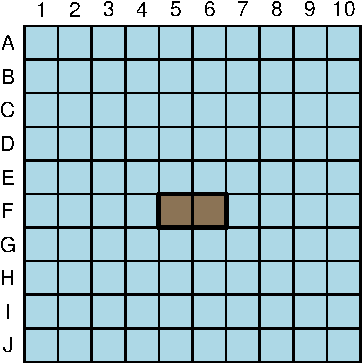
\includegraphics[keepaspectratio]{005707861_stats102a_midterm_files/figure-latex/unnamed-chunk-6-1.pdf}}

\begin{Shaded}
\begin{Highlighting}[]
\NormalTok{test\_fleet2 }\OtherTok{\textless{}{-}} \FunctionTok{fleet}\NormalTok{(}\StringTok{"tester2"}\NormalTok{)}
\NormalTok{test\_fleet2 }\OtherTok{\textless{}{-}} \FunctionTok{position\_fleet}\NormalTok{(test\_fleet2)}
\FunctionTok{plot}\NormalTok{(test\_fleet2)}
\end{Highlighting}
\end{Shaded}

\pandocbounded{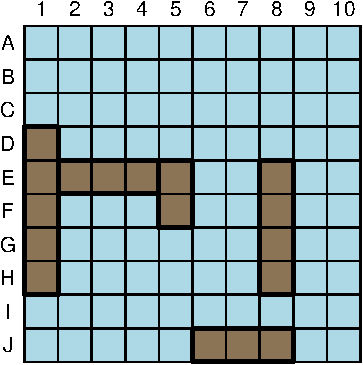
\includegraphics[keepaspectratio]{005707861_stats102a_midterm_files/figure-latex/unnamed-chunk-6-2.pdf}}

\begin{Shaded}
\begin{Highlighting}[]
\NormalTok{test\_fleet2}\SpecialCharTok{$}\NormalTok{ships[[}\DecValTok{5}\NormalTok{]]}\SpecialCharTok{$}\NormalTok{hits[}\DecValTok{1}\NormalTok{] }\OtherTok{\textless{}{-}} \ConstantTok{TRUE}
\FunctionTok{plot}\NormalTok{(test\_fleet2)}
\end{Highlighting}
\end{Shaded}

\pandocbounded{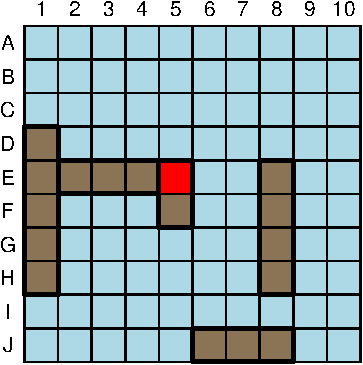
\includegraphics[keepaspectratio]{005707861_stats102a_midterm_files/figure-latex/unnamed-chunk-6-3.pdf}}

\begin{Shaded}
\begin{Highlighting}[]
\FunctionTok{summary}\NormalTok{(test\_fleet2)}
\end{Highlighting}
\end{Shaded}

\begin{verbatim}
##   Fleet Summary
##     Admiral:  tester2 
##     Ocean Size:  10 x 10 
##     Total Ships:  5 
##     Sunk Ships:  0
\end{verbatim}

\begin{Shaded}
\begin{Highlighting}[]
\NormalTok{test\_result }\OtherTok{\textless{}{-}} \FunctionTok{play\_bs}\NormalTok{(}\AttributeTok{players =} \FunctionTok{c}\NormalTok{(}\StringTok{"ai\_005707861"}\NormalTok{, }\StringTok{"ai\_005707861"}\NormalTok{))}
\FunctionTok{plot}\NormalTok{(test\_result}\SpecialCharTok{$}\NormalTok{game)}
\end{Highlighting}
\end{Shaded}

\begin{verbatim}
## Player 1's primary grid:
\end{verbatim}

\pandocbounded{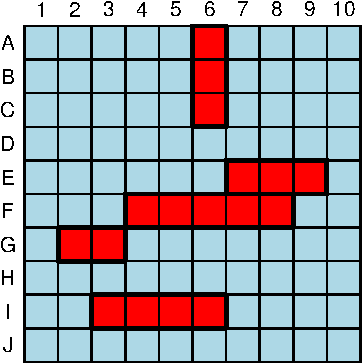
\includegraphics[keepaspectratio]{005707861_stats102a_midterm_files/figure-latex/unnamed-chunk-6-4.pdf}}

\begin{verbatim}
## Player 1's secondary grid:
\end{verbatim}

\pandocbounded{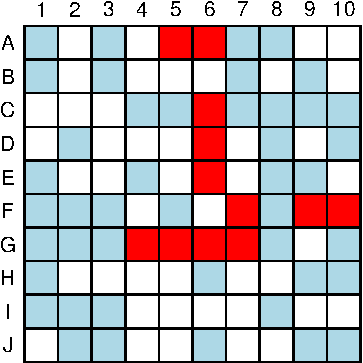
\includegraphics[keepaspectratio]{005707861_stats102a_midterm_files/figure-latex/unnamed-chunk-6-5.pdf}}

\begin{verbatim}
## Player 2's primary grid:
\end{verbatim}

\pandocbounded{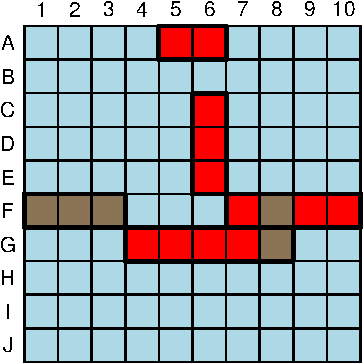
\includegraphics[keepaspectratio]{005707861_stats102a_midterm_files/figure-latex/unnamed-chunk-6-6.pdf}}

\begin{verbatim}
## Player 2's secondary grid:
\end{verbatim}

\pandocbounded{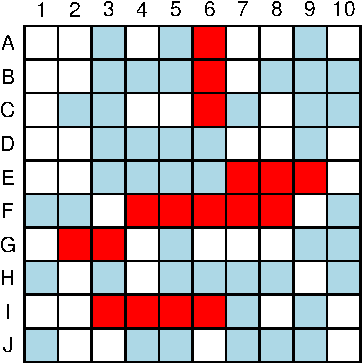
\includegraphics[keepaspectratio]{005707861_stats102a_midterm_files/figure-latex/unnamed-chunk-6-7.pdf}}

\begin{Shaded}
\begin{Highlighting}[]
\FunctionTok{summary}\NormalTok{(test\_result}\SpecialCharTok{$}\NormalTok{game)}
\end{Highlighting}
\end{Shaded}

\begin{verbatim}
## Battleship Game Summary
## Fleets:
##   Fleet Summary
##     Admiral:  ai_005707861 
##     Ocean Size:  10 x 10 
##     Total Ships:  5 
##     Sunk Ships:  5 
##   Fleet Summary
##     Admiral:  ai_005707861 
##     Ocean Size:  10 x 10 
##     Total Ships:  5 
##     Sunk Ships:  2 
## 
## Game History:
## Total Moves Made:  112 
## Total Hits:  29 
## Total Misses:  83
\end{verbatim}

\subsubsection{(4) Simulate 100,000 games for each of the following
conditions:}\label{simulate-100000-games-for-each-of-the-following-conditions}

\begin{itemize}
  \item \texttt{naive(strength = 0)} vs \texttt{naive(strength = 0)} 
  \item \texttt{naive(strength = 0)} vs \texttt{smart(strength = 9)}
  \item \texttt{smart(strength = 9)} vs \texttt{naive(strength = 0)}
  \item \texttt{smart(strength = 9)} vs \texttt{smart(strength = 9)}
\end{itemize}

\begin{Shaded}
\begin{Highlighting}[]
\CommentTok{\# (4) Simulations }
\CommentTok{\# original code took too long to run, Professor allowed me to run, save, and load the results in as RData files }

\CommentTok{\# naive(strength = 0) vs naive(strength = 0)}
\CommentTok{\# set.seed(123)}
\CommentTok{\# naive\_vs\_naive \textless{}{-} replicate(1000, play\_bs(players = c("ai\_005707861", "ai\_005707861"), }
\CommentTok{\#                                           strengths = c(0,0)))}
\CommentTok{\# save(naive\_vs\_naive, file = "naive\_vs\_naive.RData")}
\FunctionTok{load}\NormalTok{(}\StringTok{"naive\_vs\_naive.RData"}\NormalTok{)}

\CommentTok{\# naive(strength = 0) vs smart(strength = 9)}
\CommentTok{\# naive\_vs\_smart \textless{}{-} replicate(1000, play\_bs(players = c("ai\_005707861", "ai\_005707861"), }
\CommentTok{\#                                           strengths = c(0,9)))}
\CommentTok{\# save(naive\_vs\_smart, file = "naive\_vs\_smart.RData")}
\FunctionTok{load}\NormalTok{(}\StringTok{"naive\_vs\_smart.RData"}\NormalTok{)}

\CommentTok{\# smart(strength = 9) vs naive(strength = 0)}
\CommentTok{\# smart\_vs\_naive \textless{}{-} replicate(1000, play\_bs(players = c("ai\_005707861", "ai\_005707861"), }
\CommentTok{\#                                           strengths = c(9,0)))}
\CommentTok{\# save(smart\_vs\_naive, file = "smart\_vs\_naive.RData")}
\FunctionTok{load}\NormalTok{(}\StringTok{"smart\_vs\_naive.RData"}\NormalTok{)}

\CommentTok{\# smart(strength = 9) vs smart(strength = 9)}
\CommentTok{\# smart\_vs\_smart \textless{}{-} replicate(1000, play\_bs(players = c("ai\_005707861", "ai\_005707861"), }
\CommentTok{\#                                           strengths = c(9,9)))}
\CommentTok{\# save(smart\_vs\_smart, file = "smart\_vs\_smart.RData")}
\FunctionTok{load}\NormalTok{(}\StringTok{"smart\_vs\_smart.RData"}\NormalTok{)}
\end{Highlighting}
\end{Shaded}

\subsection{Questions}\label{questions}

\subsubsection{A) Showcase your game}\label{a-showcase-your-game}

Show that your functions work and that you have created a working
version of battleship.

\begin{enumerate}[label=\alph*)]
\item Create a ship called "Aircraft Carrier", a fleet with and without locations, and battleship game after 10 turns. Call your \texttt{print}, \texttt{plot}, and \texttt{summary} functions to each of them (as appropriate).
\item include a screenshot of you playing against your AI after 10 turns.
\end{enumerate}

\begin{Shaded}
\begin{Highlighting}[]
\CommentTok{\# code here}
\CommentTok{\# A)}
\NormalTok{aircraft\_carrier }\OtherTok{\textless{}{-}} \FunctionTok{ship}\NormalTok{(}\AttributeTok{name =} \StringTok{"Aircraft Carrier"}\NormalTok{, }\AttributeTok{size =} \DecValTok{5}\NormalTok{)}
\FunctionTok{print}\NormalTok{(aircraft\_carrier)}
\end{Highlighting}
\end{Shaded}

\begin{verbatim}
##   Name:  Aircraft Carrier 
##     Size:  5 
##     Position:  - 
##     Hits:  ooooo 
##     Sunk:  n
\end{verbatim}

\begin{Shaded}
\begin{Highlighting}[]
\NormalTok{fleet\_with\_loc }\OtherTok{\textless{}{-}} \FunctionTok{fleet}\NormalTok{(}\StringTok{"Player 1"}\NormalTok{)}
\NormalTok{fleet\_with\_loc }\OtherTok{\textless{}{-}} \FunctionTok{position\_fleet}\NormalTok{(fleet\_with\_loc)}
\FunctionTok{print}\NormalTok{(fleet\_with\_loc)}
\end{Highlighting}
\end{Shaded}

\begin{verbatim}
## Admiral:  Player 1 
##   Ocean:  10, 10 
##   Ships:
##   Name:  Aircraft Carrier 
##     Size:  5 
##     Position:  A-2, A-6 
##     Hits:  ooooo 
##     Sunk:  n 
##   Name:  Battleship 
##     Size:  4 
##     Position:  C-9, F-9 
##     Hits:  oooo 
##     Sunk:  n 
##   Name:  Destroyer 
##     Size:  3 
##     Position:  B-1, D-1 
##     Hits:  ooo 
##     Sunk:  n 
##   Name:  Submarine 
##     Size:  3 
##     Position:  E-3, E-5 
##     Hits:  ooo 
##     Sunk:  n 
##   Name:  Patrol Boat 
##     Size:  2 
##     Position:  B-6, C-6 
##     Hits:  oo 
##     Sunk:  n
\end{verbatim}

\begin{Shaded}
\begin{Highlighting}[]
\FunctionTok{plot}\NormalTok{(fleet\_with\_loc)}
\end{Highlighting}
\end{Shaded}

\pandocbounded{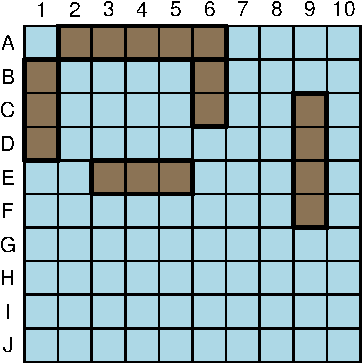
\includegraphics[keepaspectratio]{005707861_stats102a_midterm_files/figure-latex/unnamed-chunk-8-1.pdf}}

\begin{Shaded}
\begin{Highlighting}[]
\FunctionTok{summary}\NormalTok{(fleet\_with\_loc)}
\end{Highlighting}
\end{Shaded}

\begin{verbatim}
##   Fleet Summary
##     Admiral:  Player 1 
##     Ocean Size:  10 x 10 
##     Total Ships:  5 
##     Sunk Ships:  0
\end{verbatim}

\begin{Shaded}
\begin{Highlighting}[]
\NormalTok{fleet\_without\_loc }\OtherTok{\textless{}{-}} \FunctionTok{fleet}\NormalTok{(}\StringTok{"Player 1"}\NormalTok{)}
\FunctionTok{print}\NormalTok{(fleet\_without\_loc)}
\end{Highlighting}
\end{Shaded}

\begin{verbatim}
## Admiral:  Player 1 
##   Ocean:  10, 10 
##   Ships:
##   Name:  Aircraft Carrier 
##     Size:  5 
##     Position:  - 
##     Hits:  ooooo 
##     Sunk:  n 
##   Name:  Battleship 
##     Size:  4 
##     Position:  - 
##     Hits:  oooo 
##     Sunk:  n 
##   Name:  Destroyer 
##     Size:  3 
##     Position:  - 
##     Hits:  ooo 
##     Sunk:  n 
##   Name:  Submarine 
##     Size:  3 
##     Position:  - 
##     Hits:  ooo 
##     Sunk:  n 
##   Name:  Patrol Boat 
##     Size:  2 
##     Position:  - 
##     Hits:  oo 
##     Sunk:  n
\end{verbatim}

\begin{Shaded}
\begin{Highlighting}[]
\FunctionTok{plot}\NormalTok{(fleet\_without\_loc)}
\end{Highlighting}
\end{Shaded}

\pandocbounded{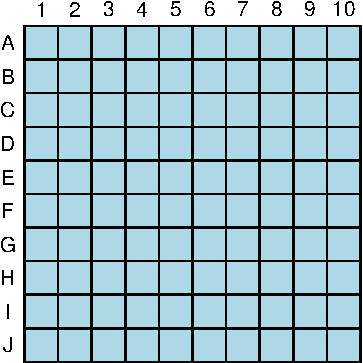
\includegraphics[keepaspectratio]{005707861_stats102a_midterm_files/figure-latex/unnamed-chunk-8-2.pdf}}

\begin{Shaded}
\begin{Highlighting}[]
\FunctionTok{summary}\NormalTok{(fleet\_without\_loc)}
\end{Highlighting}
\end{Shaded}

\begin{verbatim}
##   Fleet Summary
##     Admiral:  Player 1 
##     Ocean Size:  10 x 10 
##     Total Ships:  5 
##     Sunk Ships:  0
\end{verbatim}

\begin{Shaded}
\begin{Highlighting}[]
\CommentTok{\# function to create battleship object after 10 turns}
\NormalTok{play\_bs\_ten\_turns }\OtherTok{\textless{}{-}} \ControlFlowTok{function}\NormalTok{(}\AttributeTok{players =} \FunctionTok{c}\NormalTok{(}\StringTok{"ai\_005707861"}\NormalTok{, }\StringTok{"ai\_005707861"}\NormalTok{), }\AttributeTok{strengths =} \FunctionTok{c}\NormalTok{(}\DecValTok{9}\NormalTok{, }\DecValTok{9}\NormalTok{), }
                    \AttributeTok{verbose =} \ConstantTok{FALSE}\NormalTok{, }\AttributeTok{plot\_before\_turn =} \StringTok{"none"}\NormalTok{) \{ }
  
\NormalTok{  game }\OtherTok{\textless{}{-}} \FunctionTok{battleship}\NormalTok{() }
  
\NormalTok{  used\_coords }\OtherTok{\textless{}{-}} \FunctionTok{list}\NormalTok{()}
  \CommentTok{\# position fleets}
\NormalTok{  game}\SpecialCharTok{$}\NormalTok{fleets[[}\DecValTok{1}\NormalTok{]] }\OtherTok{\textless{}{-}}
    \FunctionTok{ai\_005707861}\NormalTok{(game}\SpecialCharTok{$}\NormalTok{fleets[[}\DecValTok{1}\NormalTok{]]) }\CommentTok{\# this positions fleet}
\NormalTok{  used\_coords[[}\DecValTok{1}\NormalTok{]] }\OtherTok{\textless{}{-}}
    \FunctionTok{lapply}\NormalTok{(game}\SpecialCharTok{$}\NormalTok{fleets[[}\DecValTok{1}\NormalTok{]]}\SpecialCharTok{$}\NormalTok{ships, }\ControlFlowTok{function}\NormalTok{(ship) \{}
      \FunctionTok{expand\_position}\NormalTok{(ship}\SpecialCharTok{$}\NormalTok{position)}
\NormalTok{  \})}
\NormalTok{  game}\SpecialCharTok{$}\NormalTok{fleets[[}\DecValTok{2}\NormalTok{]] }\OtherTok{\textless{}{-}} \FunctionTok{ai\_005707861}\NormalTok{(game}\SpecialCharTok{$}\NormalTok{fleets[[}\DecValTok{2}\NormalTok{]])}
\NormalTok{  used\_coords[[}\DecValTok{2}\NormalTok{]] }\OtherTok{\textless{}{-}} \FunctionTok{lapply}\NormalTok{(game}\SpecialCharTok{$}\NormalTok{fleets[[}\DecValTok{2}\NormalTok{]]}\SpecialCharTok{$}\NormalTok{ships, }\ControlFlowTok{function}\NormalTok{(ship) \{}
    \FunctionTok{expand\_position}\NormalTok{(ship}\SpecialCharTok{$}\NormalTok{position)}
\NormalTok{  \})}

  \CommentTok{\# game play starts here}
\NormalTok{  turn }\OtherTok{\textless{}{-}} \DecValTok{1}
\NormalTok{  memory }\OtherTok{\textless{}{-}} \FunctionTok{list}\NormalTok{() }\CommentTok{\# first comp for player1, second for player2}
  
  \ControlFlowTok{while}\NormalTok{ (turn }\SpecialCharTok{\textless{}=} \DecValTok{10}\NormalTok{) \{}
\NormalTok{    current\_player }\OtherTok{\textless{}{-}} \FunctionTok{ifelse}\NormalTok{(turn }\SpecialCharTok{\%\%} \DecValTok{2}\NormalTok{, }\DecValTok{1}\NormalTok{, }\DecValTok{2}\NormalTok{)}
\NormalTok{    opponent\_player }\OtherTok{\textless{}{-}} \FunctionTok{ifelse}\NormalTok{(turn }\SpecialCharTok{\%\%} \DecValTok{2}\NormalTok{, }\DecValTok{2}\NormalTok{, }\DecValTok{1}\NormalTok{)}
\NormalTok{    current\_admiral }\OtherTok{\textless{}{-}}\NormalTok{ game}\SpecialCharTok{$}\NormalTok{fleets[[current\_player]]}\SpecialCharTok{$}\NormalTok{admiral }\CommentTok{\# name}
\NormalTok{    opponent\_admiral }\OtherTok{\textless{}{-}}\NormalTok{ game}\SpecialCharTok{$}\NormalTok{fleets[[opponent\_player]]}\SpecialCharTok{$}\NormalTok{admiral}
    
    \ControlFlowTok{if}\NormalTok{ (plot\_before\_turn }\SpecialCharTok{\%in\%} \FunctionTok{c}\NormalTok{(}\StringTok{"both"}\NormalTok{, }\StringTok{"player1"}\NormalTok{, }\StringTok{"player2"}\NormalTok{)) \{}
      \FunctionTok{plot}\NormalTok{(game, }\AttributeTok{which =}\NormalTok{ plot\_before\_turn)}
\NormalTok{    \}}
    
    \ControlFlowTok{if}\NormalTok{ (}\FunctionTok{length}\NormalTok{(memory) }\SpecialCharTok{\textless{}=} \DecValTok{1}\NormalTok{) \{}
      \CommentTok{\# size arg not used}
\NormalTok{      result }\OtherTok{\textless{}{-}}
        \FunctionTok{ai\_005707861}\NormalTok{(game,}
\NormalTok{                     game}\SpecialCharTok{$}\NormalTok{history,}
\NormalTok{                     game}\SpecialCharTok{$}\NormalTok{fleets[[opponent\_player]]}\SpecialCharTok{$}\NormalTok{ocean,}
                     \FunctionTok{numeric}\NormalTok{(}\DecValTok{0}\NormalTok{),}
\NormalTok{                     strengths[current\_player])}
\NormalTok{    \} }\ControlFlowTok{else}\NormalTok{ \{}
\NormalTok{      result }\OtherTok{\textless{}{-}}
        \FunctionTok{ai\_005707861}\NormalTok{(game,}
\NormalTok{                     game}\SpecialCharTok{$}\NormalTok{history,}
\NormalTok{                     game}\SpecialCharTok{$}\NormalTok{fleets[[opponent\_player]]}\SpecialCharTok{$}\NormalTok{ocean,}
                     \FunctionTok{numeric}\NormalTok{(}\DecValTok{0}\NormalTok{),}
\NormalTok{                     strengths[current\_player],}
\NormalTok{                     memory[[current\_player]])}
\NormalTok{    \}}
\NormalTok{    memory[[current\_player]] }\OtherTok{\textless{}{-}}\NormalTok{ result}\SpecialCharTok{$}\NormalTok{memory}
\NormalTok{    target }\OtherTok{\textless{}{-}}\NormalTok{ result}\SpecialCharTok{$}\NormalTok{target}

\NormalTok{    hit }\OtherTok{\textless{}{-}} \ConstantTok{FALSE}
    \ControlFlowTok{for}\NormalTok{ (i }\ControlFlowTok{in} \FunctionTok{seq\_along}\NormalTok{(used\_coords[[opponent\_player]])) \{}
      \ControlFlowTok{if}\NormalTok{ (target }\SpecialCharTok{\%in\%}\NormalTok{ used\_coords[[opponent\_player]][[i]]) \{}
\NormalTok{        game}\SpecialCharTok{$}\NormalTok{fleets[[opponent\_player]]}\SpecialCharTok{$}\NormalTok{ships[[i]]}\SpecialCharTok{$}\NormalTok{hits[used\_coords[[opponent\_player]][[i]] }\SpecialCharTok{\%in\%}\NormalTok{ target] }\OtherTok{\textless{}{-}} \ConstantTok{TRUE}
\NormalTok{        hit }\OtherTok{\textless{}{-}} \ConstantTok{TRUE}
        \ControlFlowTok{if}\NormalTok{ (}\FunctionTok{all}\NormalTok{(game}\SpecialCharTok{$}\NormalTok{fleets[[opponent\_player]]}\SpecialCharTok{$}\NormalTok{ships[[i]]}\SpecialCharTok{$}\NormalTok{hits)) \{ }\CommentTok{\# also update sunk if applicable}
\NormalTok{          game}\SpecialCharTok{$}\NormalTok{fleets[[opponent\_player]]}\SpecialCharTok{$}\NormalTok{ships[[i]]}\SpecialCharTok{$}\NormalTok{sunk }\OtherTok{\textless{}{-}} \ConstantTok{TRUE} 
\NormalTok{        \}}
\NormalTok{      \}}
\NormalTok{    \}}
    
\NormalTok{    game}\SpecialCharTok{$}\NormalTok{history }\OtherTok{\textless{}{-}} \FunctionTok{tibble}\NormalTok{(}\FunctionTok{add\_row}\NormalTok{(}
      \FunctionTok{data.frame}\NormalTok{(game}\SpecialCharTok{$}\NormalTok{history),}
      \AttributeTok{from =}\NormalTok{ players[current\_player],}
      \AttributeTok{to =}\NormalTok{ players[opponent\_player],}
      \AttributeTok{target =}\NormalTok{ target,}
      \AttributeTok{hit =}\NormalTok{ hit}
\NormalTok{    ))}
    
    \ControlFlowTok{if}\NormalTok{ (verbose) \{}
      \FunctionTok{cat}\NormalTok{(}\StringTok{"Turn"}\NormalTok{, }\FunctionTok{paste0}\NormalTok{(turn, }\StringTok{":"}\NormalTok{), current\_admiral, }\StringTok{"shot at"}\NormalTok{, target, }\StringTok{"and"}\NormalTok{, }
          \FunctionTok{ifelse}\NormalTok{(hit, }\StringTok{"hit"}\NormalTok{, }\StringTok{"missed"}\NormalTok{), }\FunctionTok{paste0}\NormalTok{(opponent\_admiral, }\StringTok{"\textquotesingle{}s"}\NormalTok{), }\StringTok{"ship.}\SpecialCharTok{\textbackslash{}n}\StringTok{"}\NormalTok{)}
\NormalTok{    \}}
    
\NormalTok{    turn }\OtherTok{\textless{}{-}}\NormalTok{ turn }\SpecialCharTok{+} \DecValTok{1}
\NormalTok{  \}}
\NormalTok{  game}
\NormalTok{\}}

\CommentTok{\# bs\_after\_ten\_turns \textless{}{-} play\_bs\_ten\_turns(c("human", "ai\_005707861"), verbose = TRUE, }
\CommentTok{\#                                         plot\_before\_turn = "player1")}

\CommentTok{\# save(bs\_after\_ten\_turns, file = "bs\_after\_ten\_turns.RData")}
\FunctionTok{load}\NormalTok{(}\StringTok{"bs\_after\_ten\_turns.RData"}\NormalTok{)}
\FunctionTok{print}\NormalTok{(bs\_after\_ten\_turns)}
\end{Highlighting}
\end{Shaded}

\begin{verbatim}
## Admiral:  Player 1 
##   Ocean:  10, 10 
##   Ships:
##   Name:  Aircraft Carrier 
##     Size:  5 
##     Position:  J-6, J-10 
##     Hits:  xxxoo 
##     Sunk:  n 
##   Name:  Battleship 
##     Size:  4 
##     Position:  G-1, J-1 
##     Hits:  oooo 
##     Sunk:  n 
##   Name:  Destroyer 
##     Size:  3 
##     Position:  F-4, H-4 
##     Hits:  ooo 
##     Sunk:  n 
##   Name:  Submarine 
##     Size:  3 
##     Position:  C-4, C-6 
##     Hits:  ooo 
##     Sunk:  n 
##   Name:  Patrol Boat 
##     Size:  2 
##     Position:  F-6, G-6 
##     Hits:  oo 
##     Sunk:  n 
## 
## Admiral:  Player 2 
##   Ocean:  10, 10 
##   Ships:
##   Name:  Aircraft Carrier 
##     Size:  5 
##     Position:  A-9, E-9 
##     Hits:  xxxoo 
##     Sunk:  n 
##   Name:  Battleship 
##     Size:  4 
##     Position:  A-1, D-1 
##     Hits:  oooo 
##     Sunk:  n 
##   Name:  Destroyer 
##     Size:  3 
##     Position:  D-8, F-8 
##     Hits:  ooo 
##     Sunk:  n 
##   Name:  Submarine 
##     Size:  3 
##     Position:  H-4, H-6 
##     Hits:  ooo 
##     Sunk:  n 
##   Name:  Patrol Boat 
##     Size:  2 
##     Position:  B-2, B-3 
##     Hits:  oo 
##     Sunk:  n 
## 
## History:
## Turn 1: From Player 1 to Player 2: C-9. Result:  hit 
## Turn 2: From Player 2 to Player 1: J-8. Result:  hit 
## Turn 3: From Player 1 to Player 2: C-10. Result:  missed 
## Turn 4: From Player 2 to Player 1: J-7. Result:  hit 
## Turn 5: From Player 1 to Player 2: C-8. Result:  missed 
## Turn 6: From Player 2 to Player 1: J-6. Result:  hit 
## Turn 7: From Player 1 to Player 2: B-9. Result:  hit 
## Turn 8: From Player 2 to Player 1: J-5. Result:  missed 
## Turn 9: From Player 1 to Player 2: A-9. Result:  hit 
## Turn 10: From Player 2 to Player 1: C-10. Result:  missed
\end{verbatim}

\begin{Shaded}
\begin{Highlighting}[]
\FunctionTok{plot}\NormalTok{(bs\_after\_ten\_turns)}
\end{Highlighting}
\end{Shaded}

\begin{verbatim}
## Player 1's primary grid:
\end{verbatim}

\pandocbounded{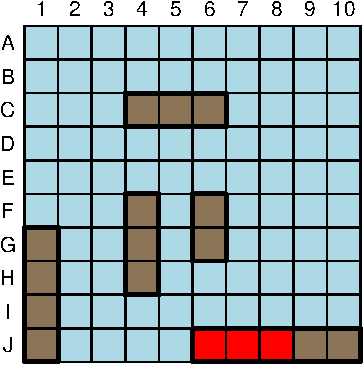
\includegraphics[keepaspectratio]{005707861_stats102a_midterm_files/figure-latex/unnamed-chunk-9-1.pdf}}

\begin{verbatim}
## Player 1's secondary grid:
\end{verbatim}

\pandocbounded{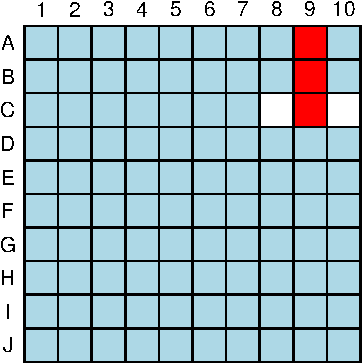
\includegraphics[keepaspectratio]{005707861_stats102a_midterm_files/figure-latex/unnamed-chunk-9-2.pdf}}

\begin{verbatim}
## Player 2's primary grid:
\end{verbatim}

\pandocbounded{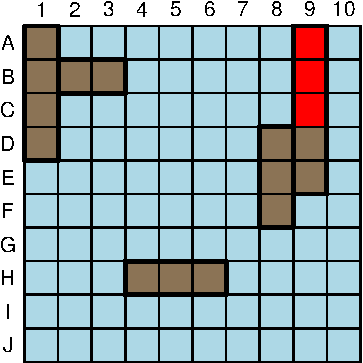
\includegraphics[keepaspectratio]{005707861_stats102a_midterm_files/figure-latex/unnamed-chunk-9-3.pdf}}

\begin{verbatim}
## Player 2's secondary grid:
\end{verbatim}

\pandocbounded{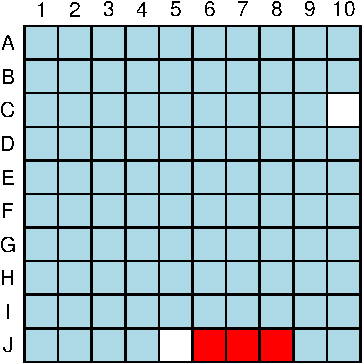
\includegraphics[keepaspectratio]{005707861_stats102a_midterm_files/figure-latex/unnamed-chunk-9-4.pdf}}

\begin{Shaded}
\begin{Highlighting}[]
\FunctionTok{summary}\NormalTok{(bs\_after\_ten\_turns)}
\end{Highlighting}
\end{Shaded}

\begin{verbatim}
## Battleship Game Summary
## Fleets:
##   Fleet Summary
##     Admiral:  Player 1 
##     Ocean Size:  10 x 10 
##     Total Ships:  5 
##     Sunk Ships:  0 
##   Fleet Summary
##     Admiral:  Player 2 
##     Ocean Size:  10 x 10 
##     Total Ships:  5 
##     Sunk Ships:  0 
## 
## Game History:
## Total Moves Made:  10 
## Total Hits:  6 
## Total Misses:  4
\end{verbatim}

\pandocbounded{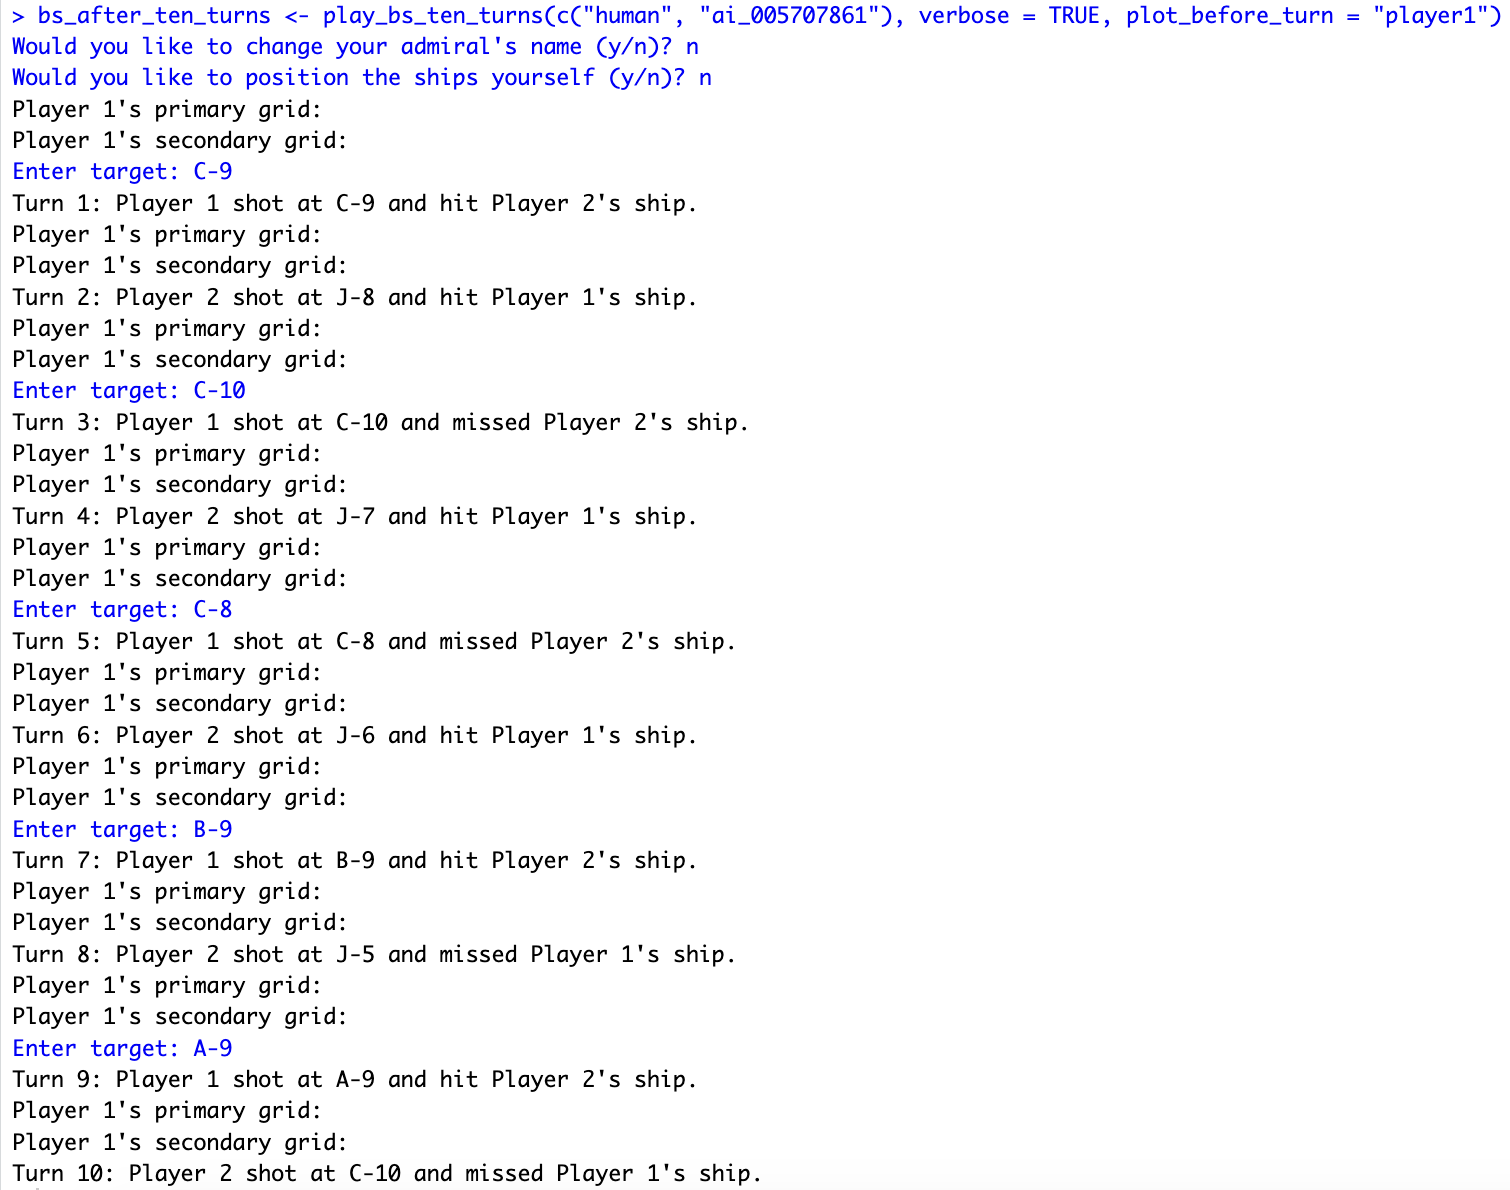
\includegraphics[keepaspectratio]{10 turns.png}}

\subsubsection{B) Standard Game
Simulations}\label{b-standard-game-simulations}

Answer the following questions for each of your simulations in (4):

\begin{enumerate}[label=\alph*)]
\item What is the minimum number of turns the winning player needed to win the game? How does this compare to a theoretical minimum.
\item What is the maximum number of turns the winning player needed to win the game? How does this compare to a theoretical maximum.
\item What is the distribution of the number of unsunk ships the winning player had remaining?
\item What is the distribution of the number of hits the losing player made?
\item In what proportion of games has the winner lost their Patrol Boat?
\item In what proportion of games is the losing player's last ship the Patrol Boat?
\end{enumerate}

\begin{Shaded}
\begin{Highlighting}[]
\CommentTok{\# naive(strength = 0) vs naive(strength = 0)}

\CommentTok{\# a)}
\FunctionTok{min}\NormalTok{(}\FunctionTok{sapply}\NormalTok{(naive\_vs\_naive[}\DecValTok{2}\NormalTok{, ], }\ControlFlowTok{function}\NormalTok{(comp) }\FunctionTok{nrow}\NormalTok{(comp}\SpecialCharTok{$}\NormalTok{history)))}
\end{Highlighting}
\end{Shaded}

\begin{verbatim}
## [1] 127
\end{verbatim}

\subsubsection{In an ideal scenario the player would win in 17 turns (if
they hit a ship every time they go). Going back and forth, the
theorectical minimum is 33 turns if that same player goes first. The
actual minimum of 127 is much higher than the theoretical
minimum.}\label{in-an-ideal-scenario-the-player-would-win-in-17-turns-if-they-hit-a-ship-every-time-they-go.-going-back-and-forth-the-theorectical-minimum-is-33-turns-if-that-same-player-goes-first.-the-actual-minimum-of-127-is-much-higher-than-the-theoretical-minimum.}

\begin{Shaded}
\begin{Highlighting}[]
\CommentTok{\# b)}
\FunctionTok{max}\NormalTok{(}\FunctionTok{sapply}\NormalTok{(naive\_vs\_naive[}\DecValTok{2}\NormalTok{, ], }\ControlFlowTok{function}\NormalTok{(comp) }\FunctionTok{nrow}\NormalTok{(comp}\SpecialCharTok{$}\NormalTok{history)))}
\end{Highlighting}
\end{Shaded}

\begin{verbatim}
## [1] 199
\end{verbatim}

\subsubsection{In the worst case scenario the player would win in 50
turns (if they go first). Going back and forth, the theorectical maximum
is 199 turns if that same player goes first. The actual maximum of 199
is equal to the theoretical
minimum.}\label{in-the-worst-case-scenario-the-player-would-win-in-50-turns-if-they-go-first.-going-back-and-forth-the-theorectical-maximum-is-199-turns-if-that-same-player-goes-first.-the-actual-maximum-of-199-is-equal-to-the-theoretical-minimum.}

\begin{Shaded}
\begin{Highlighting}[]
\CommentTok{\# c)}
\NormalTok{unsunk\_ships }\OtherTok{\textless{}{-}} \FunctionTok{sapply}\NormalTok{(}\DecValTok{1}\SpecialCharTok{:}\DecValTok{1000}\NormalTok{, }\ControlFlowTok{function}\NormalTok{ (i) \{}
\NormalTok{  winner }\OtherTok{\textless{}{-}} \FunctionTok{ifelse}\NormalTok{(}\FunctionTok{nrow}\NormalTok{(naive\_vs\_naive[[}\DecValTok{2}\NormalTok{, i]]}\SpecialCharTok{$}\NormalTok{history) }\SpecialCharTok{\%\%} \DecValTok{2}\NormalTok{, }\DecValTok{1}\NormalTok{, }\DecValTok{2}\NormalTok{) }\CommentTok{\# 1 or 2}
  \FunctionTok{sum}\NormalTok{(}\FunctionTok{sapply}\NormalTok{(naive\_vs\_naive[[}\DecValTok{2}\NormalTok{, i]]}\SpecialCharTok{$}\NormalTok{fleets[[winner]]}\SpecialCharTok{$}\NormalTok{ships, }\ControlFlowTok{function}\NormalTok{(comp) \{}
    \SpecialCharTok{!}\NormalTok{comp}\SpecialCharTok{$}\NormalTok{sunk}
\NormalTok{  \}))}
\NormalTok{\})}

\NormalTok{unsunk\_ships\_df }\OtherTok{\textless{}{-}} \FunctionTok{data.frame}\NormalTok{(unsunk\_ships)}

\CommentTok{\# Plot the distribution using ggplot2}
\FunctionTok{ggplot}\NormalTok{(unsunk\_ships\_df, }\FunctionTok{aes}\NormalTok{(}\AttributeTok{x =} \FunctionTok{factor}\NormalTok{(unsunk\_ships))) }\SpecialCharTok{+}
  \FunctionTok{geom\_bar}\NormalTok{(}\AttributeTok{fill =} \StringTok{"lightblue"}\NormalTok{, }\AttributeTok{color =} \StringTok{"black"}\NormalTok{) }\SpecialCharTok{+}
  \FunctionTok{labs}\NormalTok{(}\AttributeTok{title =} \StringTok{"Distribution of Unsunk Ships for Winning Player"}\NormalTok{, }
       \AttributeTok{x =} \StringTok{"Number of Unsunk Ships"}\NormalTok{, }
       \AttributeTok{y =} \StringTok{"Frequency"}\NormalTok{) }\SpecialCharTok{+}
  \FunctionTok{theme\_minimal}\NormalTok{()}
\end{Highlighting}
\end{Shaded}

\pandocbounded{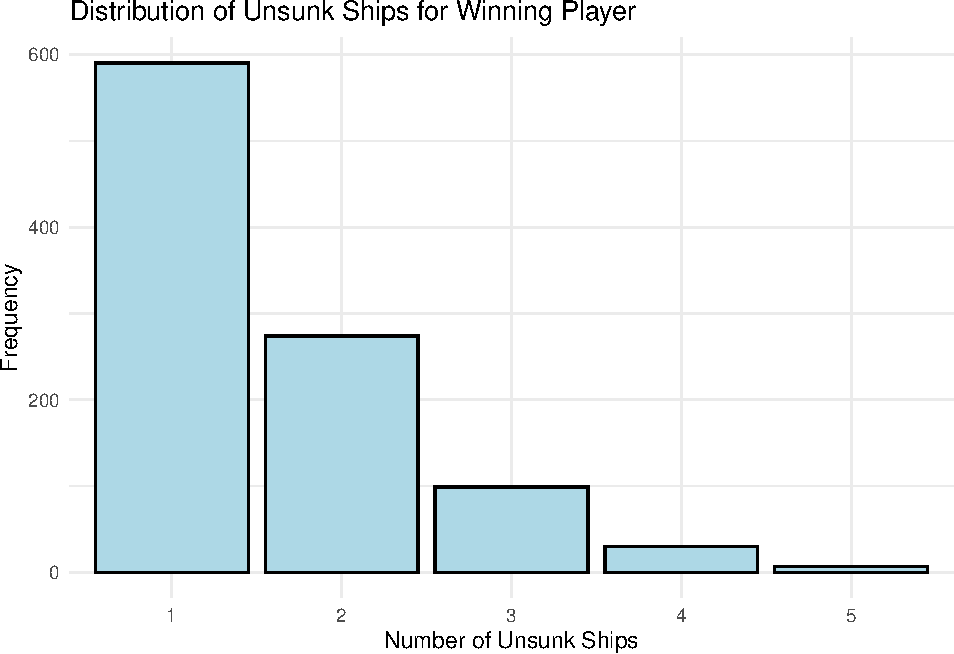
\includegraphics[keepaspectratio]{005707861_stats102a_midterm_files/figure-latex/unnamed-chunk-12-1.pdf}}

\subsubsection{The distribution of the number of unsunk ships the
winning player had remaining is
right-skewed.}\label{the-distribution-of-the-number-of-unsunk-ships-the-winning-player-had-remaining-is-right-skewed.}

\begin{Shaded}
\begin{Highlighting}[]
\CommentTok{\# d)}
\NormalTok{hits\_lp }\OtherTok{\textless{}{-}} \FunctionTok{sapply}\NormalTok{(}\DecValTok{1}\SpecialCharTok{:}\DecValTok{1000}\NormalTok{, }\ControlFlowTok{function}\NormalTok{ (i) \{}
\NormalTok{  winner }\OtherTok{\textless{}{-}} \FunctionTok{ifelse}\NormalTok{(}\FunctionTok{nrow}\NormalTok{(naive\_vs\_naive[[}\DecValTok{2}\NormalTok{, i]]}\SpecialCharTok{$}\NormalTok{history) }\SpecialCharTok{\%\%} \DecValTok{2}\NormalTok{, }\DecValTok{1}\NormalTok{, }\DecValTok{2}\NormalTok{) }\CommentTok{\# 1 or 2}
  \FunctionTok{sum}\NormalTok{(}\FunctionTok{sapply}\NormalTok{(naive\_vs\_naive[[}\DecValTok{2}\NormalTok{, i]]}\SpecialCharTok{$}\NormalTok{fleets[[winner]]}\SpecialCharTok{$}\NormalTok{ships, }\ControlFlowTok{function}\NormalTok{(comp) \{}
    \FunctionTok{sum}\NormalTok{(comp}\SpecialCharTok{$}\NormalTok{hits)}
\NormalTok{  \}))}
\NormalTok{\})}

\NormalTok{hits\_lp\_df }\OtherTok{\textless{}{-}} \FunctionTok{data.frame}\NormalTok{(hits\_lp)}

\CommentTok{\# Plot the distribution using ggplot2}
\FunctionTok{ggplot}\NormalTok{(hits\_lp\_df, }\FunctionTok{aes}\NormalTok{(}\AttributeTok{x =} \FunctionTok{factor}\NormalTok{(hits\_lp))) }\SpecialCharTok{+}
  \FunctionTok{geom\_bar}\NormalTok{(}\AttributeTok{fill =} \StringTok{"lightblue"}\NormalTok{, }\AttributeTok{color =} \StringTok{"black"}\NormalTok{) }\SpecialCharTok{+}
  \FunctionTok{labs}\NormalTok{(}\AttributeTok{title =} \StringTok{"Distribution of Hits Losing Player Made"}\NormalTok{, }
       \AttributeTok{x =} \StringTok{"Number of Hits"}\NormalTok{, }
       \AttributeTok{y =} \StringTok{"Frequency"}\NormalTok{) }\SpecialCharTok{+}
  \FunctionTok{theme\_minimal}\NormalTok{()}
\end{Highlighting}
\end{Shaded}

\pandocbounded{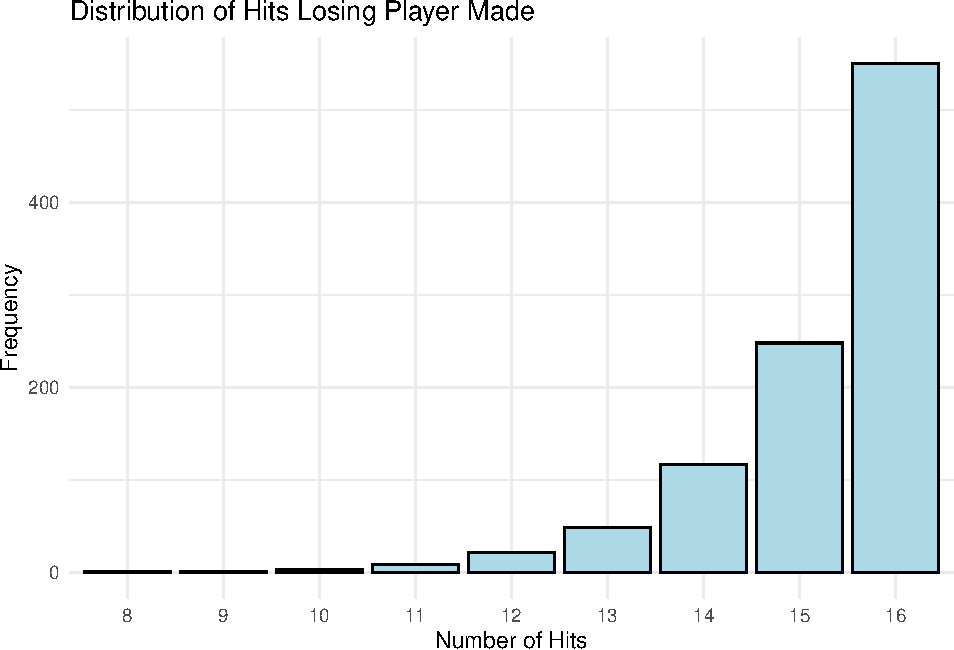
\includegraphics[keepaspectratio]{005707861_stats102a_midterm_files/figure-latex/unnamed-chunk-13-1.pdf}}

\subsubsection{The distribution of the number of hits the losing player
made is left-skewed with a minimum of 8 and maximum of
16.}\label{the-distribution-of-the-number-of-hits-the-losing-player-made-is-left-skewed-with-a-minimum-of-8-and-maximum-of-16.}

\begin{Shaded}
\begin{Highlighting}[]
\CommentTok{\# e)}
\NormalTok{patrol\_boats\_lost }\OtherTok{\textless{}{-}} \FunctionTok{sum}\NormalTok{(}\FunctionTok{sapply}\NormalTok{(}\DecValTok{1}\SpecialCharTok{:}\DecValTok{1000}\NormalTok{, }\ControlFlowTok{function}\NormalTok{ (i) \{}
\NormalTok{  winner }\OtherTok{\textless{}{-}} \FunctionTok{ifelse}\NormalTok{(}\FunctionTok{nrow}\NormalTok{(naive\_vs\_naive[[}\DecValTok{2}\NormalTok{, i]]}\SpecialCharTok{$}\NormalTok{history) }\SpecialCharTok{\%\%} \DecValTok{2}\NormalTok{, }\DecValTok{1}\NormalTok{, }\DecValTok{2}\NormalTok{) }\CommentTok{\# 1 or 2}
\NormalTok{  naive\_vs\_naive[[}\DecValTok{2}\NormalTok{, i]]}\SpecialCharTok{$}\NormalTok{fleets[[winner]]}\SpecialCharTok{$}\NormalTok{ships[[}\DecValTok{5}\NormalTok{]]}\SpecialCharTok{$}\NormalTok{sunk}
\NormalTok{\}))}

\NormalTok{(prop\_patrol\_boats\_lost }\OtherTok{\textless{}{-}}\NormalTok{ patrol\_boats\_lost }\SpecialCharTok{/} \DecValTok{1000}\NormalTok{)}
\end{Highlighting}
\end{Shaded}

\begin{verbatim}
## [1] 0.795
\end{verbatim}

\subsubsection{The proportion of games in which the winner lost their
Patrol Boat is
0.795.}\label{the-proportion-of-games-in-which-the-winner-lost-their-patrol-boat-is-0.795.}

\begin{Shaded}
\begin{Highlighting}[]
\CommentTok{\# f)}
\NormalTok{last\_ship\_patrol }\OtherTok{\textless{}{-}} \FunctionTok{sum}\NormalTok{(}\FunctionTok{sapply}\NormalTok{(}\DecValTok{1}\SpecialCharTok{:}\DecValTok{1000}\NormalTok{, }\ControlFlowTok{function}\NormalTok{ (i) \{}
\NormalTok{  comp }\OtherTok{\textless{}{-}}\NormalTok{ naive\_vs\_naive[[}\DecValTok{2}\NormalTok{, i]]}
\NormalTok{  winner }\OtherTok{\textless{}{-}} \FunctionTok{ifelse}\NormalTok{(}\FunctionTok{nrow}\NormalTok{(comp}\SpecialCharTok{$}\NormalTok{history) }\SpecialCharTok{\%\%} \DecValTok{2}\NormalTok{, }\DecValTok{1}\NormalTok{, }\DecValTok{2}\NormalTok{) }\CommentTok{\# 1 or 2}
\NormalTok{  patrol\_boat\_position }\OtherTok{\textless{}{-}}
\NormalTok{    comp}\SpecialCharTok{$}\NormalTok{fleets[[}\FunctionTok{ifelse}\NormalTok{(winner }\SpecialCharTok{==} \DecValTok{1}\NormalTok{, }\DecValTok{2}\NormalTok{, }\DecValTok{1}\NormalTok{)]]}\SpecialCharTok{$}\NormalTok{ships[[}\DecValTok{5}\NormalTok{]]}\SpecialCharTok{$}\NormalTok{position}
\NormalTok{  last\_target }\OtherTok{\textless{}{-}}\NormalTok{ comp}\SpecialCharTok{$}\NormalTok{history }\SpecialCharTok{\%\textgreater{}\%} \FunctionTok{pull}\NormalTok{(target) }\SpecialCharTok{\%\textgreater{}\%} \FunctionTok{tail}\NormalTok{(}\DecValTok{1}\NormalTok{)}
\NormalTok{  last\_target }\SpecialCharTok{\%in\%}\NormalTok{ patrol\_boat\_position}
\NormalTok{\}))}

\NormalTok{(prop\_last\_ship\_patrol }\OtherTok{\textless{}{-}}\NormalTok{ last\_ship\_patrol }\SpecialCharTok{/} \DecValTok{1000}\NormalTok{)}
\end{Highlighting}
\end{Shaded}

\begin{verbatim}
## [1] 0.111
\end{verbatim}

\subsubsection{The proportion of games in which the last ship of the
losing player is their Patrol Boat is
0.111.}\label{the-proportion-of-games-in-which-the-last-ship-of-the-losing-player-is-their-patrol-boat-is-0.111.}

\begin{Shaded}
\begin{Highlighting}[]
\CommentTok{\# naive(strength = 0) vs smart(strength = 9)}

\CommentTok{\# a)}
\FunctionTok{min}\NormalTok{(}\FunctionTok{sapply}\NormalTok{(naive\_vs\_smart[}\DecValTok{2}\NormalTok{, ], }\ControlFlowTok{function}\NormalTok{(comp) }\FunctionTok{nrow}\NormalTok{(comp}\SpecialCharTok{$}\NormalTok{history)))}
\end{Highlighting}
\end{Shaded}

\begin{verbatim}
## [1] 58
\end{verbatim}

\subsubsection{In an ideal scenario the player would win in 17 turns (if
they hit a ship every time they go). Going back and forth, the
theorectical minimum is 33 turns if that same player goes first. The
actual minimum of 58 is higher than the theoretical minimum but much
better than the naive vs.~naive actual minimum of
127.}\label{in-an-ideal-scenario-the-player-would-win-in-17-turns-if-they-hit-a-ship-every-time-they-go.-going-back-and-forth-the-theorectical-minimum-is-33-turns-if-that-same-player-goes-first.-the-actual-minimum-of-58-is-higher-than-the-theoretical-minimum-but-much-better-than-the-naive-vs.-naive-actual-minimum-of-127.}

\begin{Shaded}
\begin{Highlighting}[]
\CommentTok{\# b)}
\FunctionTok{max}\NormalTok{(}\FunctionTok{sapply}\NormalTok{(naive\_vs\_smart[}\DecValTok{2}\NormalTok{, ], }\ControlFlowTok{function}\NormalTok{(comp) }\FunctionTok{nrow}\NormalTok{(comp}\SpecialCharTok{$}\NormalTok{history)))}
\end{Highlighting}
\end{Shaded}

\begin{verbatim}
## [1] 199
\end{verbatim}

\subsubsection{In the worst case scenario the player would win in 50
turns (if they go first). Going back and forth, the theorectical maximum
is 199 turns if that same player goes first. The actual maximum of 199
is equal to the theoretical
minimum.}\label{in-the-worst-case-scenario-the-player-would-win-in-50-turns-if-they-go-first.-going-back-and-forth-the-theorectical-maximum-is-199-turns-if-that-same-player-goes-first.-the-actual-maximum-of-199-is-equal-to-the-theoretical-minimum.-1}

\begin{Shaded}
\begin{Highlighting}[]
\CommentTok{\# c)}
\NormalTok{unsunk\_ships }\OtherTok{\textless{}{-}} \FunctionTok{sapply}\NormalTok{(}\DecValTok{1}\SpecialCharTok{:}\DecValTok{1000}\NormalTok{, }\ControlFlowTok{function}\NormalTok{ (i) \{}
\NormalTok{  winner }\OtherTok{\textless{}{-}} \FunctionTok{ifelse}\NormalTok{(}\FunctionTok{nrow}\NormalTok{(naive\_vs\_smart[[}\DecValTok{2}\NormalTok{, i]]}\SpecialCharTok{$}\NormalTok{history) }\SpecialCharTok{\%\%} \DecValTok{2}\NormalTok{, }\DecValTok{1}\NormalTok{, }\DecValTok{2}\NormalTok{) }\CommentTok{\# 1 or 2}
  \FunctionTok{sum}\NormalTok{(}\FunctionTok{sapply}\NormalTok{(naive\_vs\_smart[[}\DecValTok{2}\NormalTok{, i]]}\SpecialCharTok{$}\NormalTok{fleets[[winner]]}\SpecialCharTok{$}\NormalTok{ships, }\ControlFlowTok{function}\NormalTok{(comp) \{}
    \SpecialCharTok{!}\NormalTok{comp}\SpecialCharTok{$}\NormalTok{sunk}
\NormalTok{  \}))}
\NormalTok{\})}

\NormalTok{unsunk\_ships\_df }\OtherTok{\textless{}{-}} \FunctionTok{data.frame}\NormalTok{(unsunk\_ships)}

\CommentTok{\# Plot the distribution using ggplot2}
\FunctionTok{ggplot}\NormalTok{(unsunk\_ships\_df, }\FunctionTok{aes}\NormalTok{(}\AttributeTok{x =} \FunctionTok{factor}\NormalTok{(unsunk\_ships))) }\SpecialCharTok{+}
  \FunctionTok{geom\_bar}\NormalTok{(}\AttributeTok{fill =} \StringTok{"lightblue"}\NormalTok{, }\AttributeTok{color =} \StringTok{"black"}\NormalTok{) }\SpecialCharTok{+}
  \FunctionTok{labs}\NormalTok{(}\AttributeTok{title =} \StringTok{"Distribution of Unsunk Ships for Winning Player"}\NormalTok{, }
       \AttributeTok{x =} \StringTok{"Number of Unsunk Ships"}\NormalTok{, }
       \AttributeTok{y =} \StringTok{"Frequency"}\NormalTok{) }\SpecialCharTok{+}
  \FunctionTok{theme\_minimal}\NormalTok{()}
\end{Highlighting}
\end{Shaded}

\pandocbounded{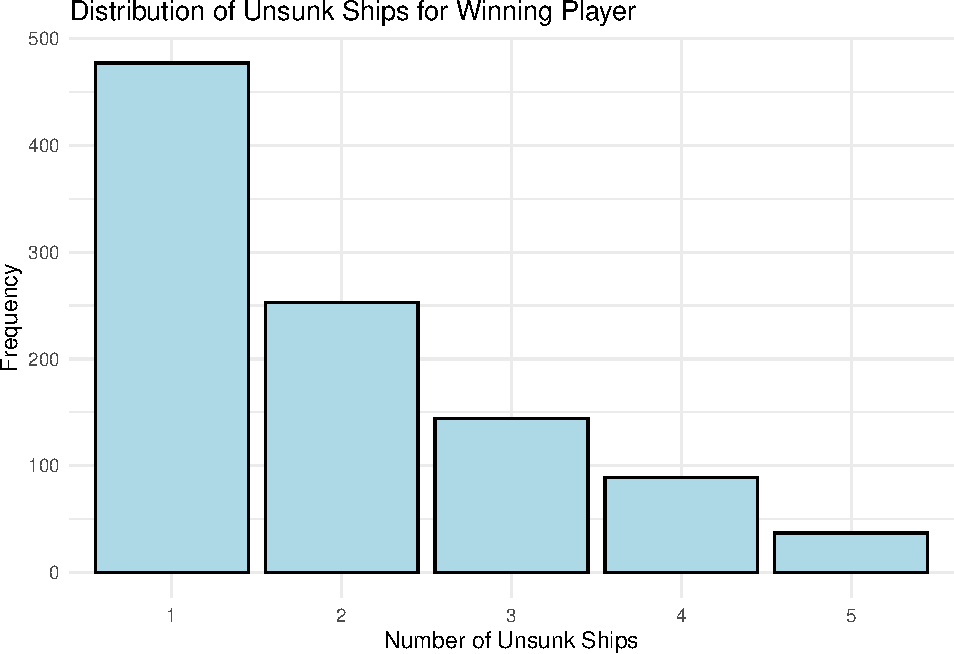
\includegraphics[keepaspectratio]{005707861_stats102a_midterm_files/figure-latex/unnamed-chunk-18-1.pdf}}

\subsubsection{The distribution of the number of unsunk ships the
winning player had remaining is
right-skewed.}\label{the-distribution-of-the-number-of-unsunk-ships-the-winning-player-had-remaining-is-right-skewed.-1}

\begin{Shaded}
\begin{Highlighting}[]
\CommentTok{\# d)}
\NormalTok{hits\_lp }\OtherTok{\textless{}{-}} \FunctionTok{sapply}\NormalTok{(}\DecValTok{1}\SpecialCharTok{:}\DecValTok{1000}\NormalTok{, }\ControlFlowTok{function}\NormalTok{ (i) \{}
\NormalTok{  winner }\OtherTok{\textless{}{-}} \FunctionTok{ifelse}\NormalTok{(}\FunctionTok{nrow}\NormalTok{(naive\_vs\_smart[[}\DecValTok{2}\NormalTok{, i]]}\SpecialCharTok{$}\NormalTok{history) }\SpecialCharTok{\%\%} \DecValTok{2}\NormalTok{, }\DecValTok{1}\NormalTok{, }\DecValTok{2}\NormalTok{) }\CommentTok{\# 1 or 2}
  \FunctionTok{sum}\NormalTok{(}\FunctionTok{sapply}\NormalTok{(naive\_vs\_smart[[}\DecValTok{2}\NormalTok{, i]]}\SpecialCharTok{$}\NormalTok{fleets[[winner]]}\SpecialCharTok{$}\NormalTok{ships, }\ControlFlowTok{function}\NormalTok{(comp) \{}
    \FunctionTok{sum}\NormalTok{(comp}\SpecialCharTok{$}\NormalTok{hits)}
\NormalTok{  \}))}
\NormalTok{\})}

\NormalTok{hits\_lp\_df }\OtherTok{\textless{}{-}} \FunctionTok{data.frame}\NormalTok{(hits\_lp)}

\CommentTok{\# Plot the distribution using ggplot2}
\FunctionTok{ggplot}\NormalTok{(hits\_lp\_df, }\FunctionTok{aes}\NormalTok{(}\AttributeTok{x =} \FunctionTok{factor}\NormalTok{(hits\_lp))) }\SpecialCharTok{+}
  \FunctionTok{geom\_bar}\NormalTok{(}\AttributeTok{fill =} \StringTok{"lightblue"}\NormalTok{, }\AttributeTok{color =} \StringTok{"black"}\NormalTok{) }\SpecialCharTok{+}
  \FunctionTok{labs}\NormalTok{(}\AttributeTok{title =} \StringTok{"Distribution of Hits Losing Player Made"}\NormalTok{, }
       \AttributeTok{x =} \StringTok{"Number of Hits"}\NormalTok{, }
       \AttributeTok{y =} \StringTok{"Frequency"}\NormalTok{) }\SpecialCharTok{+}
  \FunctionTok{theme\_minimal}\NormalTok{()}
\end{Highlighting}
\end{Shaded}

\pandocbounded{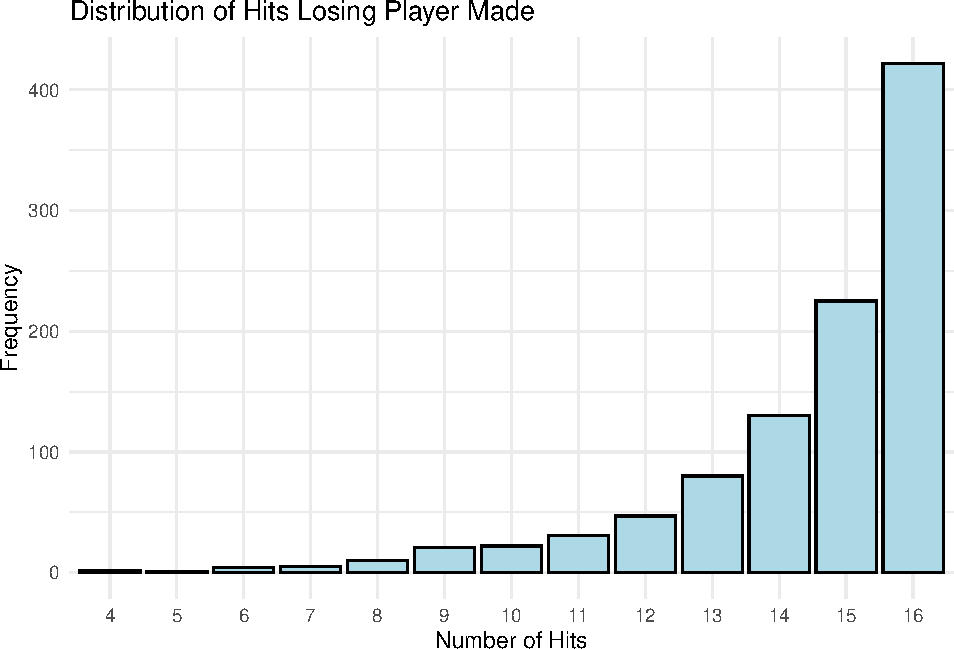
\includegraphics[keepaspectratio]{005707861_stats102a_midterm_files/figure-latex/unnamed-chunk-19-1.pdf}}

\subsubsection{The distribution of the number of hits the losing player
made is left-skewed with a minimum of 4 and maximum of
16.}\label{the-distribution-of-the-number-of-hits-the-losing-player-made-is-left-skewed-with-a-minimum-of-4-and-maximum-of-16.}

\begin{Shaded}
\begin{Highlighting}[]
\CommentTok{\# e)}
\NormalTok{patrol\_boats\_lost }\OtherTok{\textless{}{-}} \FunctionTok{sum}\NormalTok{(}\FunctionTok{sapply}\NormalTok{(}\DecValTok{1}\SpecialCharTok{:}\DecValTok{1000}\NormalTok{, }\ControlFlowTok{function}\NormalTok{ (i) \{}
\NormalTok{  winner }\OtherTok{\textless{}{-}} \FunctionTok{ifelse}\NormalTok{(}\FunctionTok{nrow}\NormalTok{(naive\_vs\_smart[[}\DecValTok{2}\NormalTok{, i]]}\SpecialCharTok{$}\NormalTok{history) }\SpecialCharTok{\%\%} \DecValTok{2}\NormalTok{, }\DecValTok{1}\NormalTok{, }\DecValTok{2}\NormalTok{) }\CommentTok{\# 1 or 2}
\NormalTok{  naive\_vs\_smart[[}\DecValTok{2}\NormalTok{, i]]}\SpecialCharTok{$}\NormalTok{fleets[[winner]]}\SpecialCharTok{$}\NormalTok{ships[[}\DecValTok{5}\NormalTok{]]}\SpecialCharTok{$}\NormalTok{sunk}
\NormalTok{\}))}

\NormalTok{(prop\_patrol\_boats\_lost }\OtherTok{\textless{}{-}}\NormalTok{ patrol\_boats\_lost }\SpecialCharTok{/} \DecValTok{1000}\NormalTok{)}
\end{Highlighting}
\end{Shaded}

\begin{verbatim}
## [1] 0.73
\end{verbatim}

\subsubsection{The proportion of games in which the winner lost their
Patrol Boat is
0.73.}\label{the-proportion-of-games-in-which-the-winner-lost-their-patrol-boat-is-0.73.}

\begin{Shaded}
\begin{Highlighting}[]
\CommentTok{\# f)}
\NormalTok{last\_ship\_patrol }\OtherTok{\textless{}{-}} \FunctionTok{sum}\NormalTok{(}\FunctionTok{sapply}\NormalTok{(}\DecValTok{1}\SpecialCharTok{:}\DecValTok{1000}\NormalTok{, }\ControlFlowTok{function}\NormalTok{ (i) \{}
\NormalTok{  comp }\OtherTok{\textless{}{-}}\NormalTok{ naive\_vs\_smart[[}\DecValTok{2}\NormalTok{, i]]}
\NormalTok{  winner }\OtherTok{\textless{}{-}} \FunctionTok{ifelse}\NormalTok{(}\FunctionTok{nrow}\NormalTok{(comp}\SpecialCharTok{$}\NormalTok{history) }\SpecialCharTok{\%\%} \DecValTok{2}\NormalTok{, }\DecValTok{1}\NormalTok{, }\DecValTok{2}\NormalTok{) }\CommentTok{\# 1 or 2}
\NormalTok{  patrol\_boat\_position }\OtherTok{\textless{}{-}}
\NormalTok{    comp}\SpecialCharTok{$}\NormalTok{fleets[[}\FunctionTok{ifelse}\NormalTok{(winner }\SpecialCharTok{==} \DecValTok{1}\NormalTok{, }\DecValTok{2}\NormalTok{, }\DecValTok{1}\NormalTok{)]]}\SpecialCharTok{$}\NormalTok{ships[[}\DecValTok{5}\NormalTok{]]}\SpecialCharTok{$}\NormalTok{position}
\NormalTok{  last\_target }\OtherTok{\textless{}{-}}\NormalTok{ comp}\SpecialCharTok{$}\NormalTok{history }\SpecialCharTok{\%\textgreater{}\%} \FunctionTok{pull}\NormalTok{(target) }\SpecialCharTok{\%\textgreater{}\%} \FunctionTok{tail}\NormalTok{(}\DecValTok{1}\NormalTok{)}
\NormalTok{  last\_target }\SpecialCharTok{\%in\%}\NormalTok{ patrol\_boat\_position}
\NormalTok{\}))}

\NormalTok{(prop\_last\_ship\_patrol }\OtherTok{\textless{}{-}}\NormalTok{ last\_ship\_patrol }\SpecialCharTok{/} \DecValTok{1000}\NormalTok{)}
\end{Highlighting}
\end{Shaded}

\begin{verbatim}
## [1] 0.16
\end{verbatim}

\subsubsection{The proportion of games in which the last ship of the
losing player is their Patrol Boat is
0.16.}\label{the-proportion-of-games-in-which-the-last-ship-of-the-losing-player-is-their-patrol-boat-is-0.16.}

\begin{Shaded}
\begin{Highlighting}[]
\CommentTok{\# smart(strength = 9) vs naive(strength = 0)}

\CommentTok{\# a)}
\FunctionTok{min}\NormalTok{(}\FunctionTok{sapply}\NormalTok{(smart\_vs\_naive[}\DecValTok{2}\NormalTok{, ], }\ControlFlowTok{function}\NormalTok{(comp) }\FunctionTok{nrow}\NormalTok{(comp}\SpecialCharTok{$}\NormalTok{history)))}
\end{Highlighting}
\end{Shaded}

\begin{verbatim}
## [1] 63
\end{verbatim}

\subsubsection{In an ideal scenario the player would win in 17 turns (if
they hit a ship every time they go). Going back and forth, the
theorectical minimum is 33 turns if that same player goes first. The
actual minimum of 63 is much higher than the theoretical
minimum.}\label{in-an-ideal-scenario-the-player-would-win-in-17-turns-if-they-hit-a-ship-every-time-they-go.-going-back-and-forth-the-theorectical-minimum-is-33-turns-if-that-same-player-goes-first.-the-actual-minimum-of-63-is-much-higher-than-the-theoretical-minimum.}

\begin{Shaded}
\begin{Highlighting}[]
\CommentTok{\# b)}
\FunctionTok{max}\NormalTok{(}\FunctionTok{sapply}\NormalTok{(smart\_vs\_naive[}\DecValTok{2}\NormalTok{, ], }\ControlFlowTok{function}\NormalTok{(comp) }\FunctionTok{nrow}\NormalTok{(comp}\SpecialCharTok{$}\NormalTok{history)))}
\end{Highlighting}
\end{Shaded}

\begin{verbatim}
## [1] 199
\end{verbatim}

\subsubsection{In the worst case scenario the player would win in 50
turns (if they go first). Going back and forth, the theorectical maximum
is 199 turns if that same player goes first. The actual maximum of 200
is equal to the theoretical
minimum.}\label{in-the-worst-case-scenario-the-player-would-win-in-50-turns-if-they-go-first.-going-back-and-forth-the-theorectical-maximum-is-199-turns-if-that-same-player-goes-first.-the-actual-maximum-of-200-is-equal-to-the-theoretical-minimum.}

\begin{Shaded}
\begin{Highlighting}[]
\CommentTok{\# c)}
\NormalTok{unsunk\_ships }\OtherTok{\textless{}{-}} \FunctionTok{sapply}\NormalTok{(}\DecValTok{1}\SpecialCharTok{:}\DecValTok{1000}\NormalTok{, }\ControlFlowTok{function}\NormalTok{ (i) \{}
\NormalTok{  winner }\OtherTok{\textless{}{-}} \FunctionTok{ifelse}\NormalTok{(}\FunctionTok{nrow}\NormalTok{(smart\_vs\_naive[[}\DecValTok{2}\NormalTok{, i]]}\SpecialCharTok{$}\NormalTok{history) }\SpecialCharTok{\%\%} \DecValTok{2}\NormalTok{, }\DecValTok{1}\NormalTok{, }\DecValTok{2}\NormalTok{) }\CommentTok{\# 1 or 2}
  \FunctionTok{sum}\NormalTok{(}\FunctionTok{sapply}\NormalTok{(smart\_vs\_naive[[}\DecValTok{2}\NormalTok{, i]]}\SpecialCharTok{$}\NormalTok{fleets[[winner]]}\SpecialCharTok{$}\NormalTok{ships, }\ControlFlowTok{function}\NormalTok{(comp) \{}
    \SpecialCharTok{!}\NormalTok{comp}\SpecialCharTok{$}\NormalTok{sunk}
\NormalTok{  \}))}
\NormalTok{\})}

\NormalTok{unsunk\_ships\_df }\OtherTok{\textless{}{-}} \FunctionTok{data.frame}\NormalTok{(unsunk\_ships)}

\CommentTok{\# Plot the distribution using ggplot2}
\FunctionTok{ggplot}\NormalTok{(unsunk\_ships\_df, }\FunctionTok{aes}\NormalTok{(}\AttributeTok{x =} \FunctionTok{factor}\NormalTok{(unsunk\_ships))) }\SpecialCharTok{+}
  \FunctionTok{geom\_bar}\NormalTok{(}\AttributeTok{fill =} \StringTok{"lightblue"}\NormalTok{, }\AttributeTok{color =} \StringTok{"black"}\NormalTok{) }\SpecialCharTok{+}
  \FunctionTok{labs}\NormalTok{(}\AttributeTok{title =} \StringTok{"Distribution of Unsunk Ships for Winning Player"}\NormalTok{, }
       \AttributeTok{x =} \StringTok{"Number of Unsunk Ships"}\NormalTok{, }
       \AttributeTok{y =} \StringTok{"Frequency"}\NormalTok{) }\SpecialCharTok{+}
  \FunctionTok{theme\_minimal}\NormalTok{()}
\end{Highlighting}
\end{Shaded}

\pandocbounded{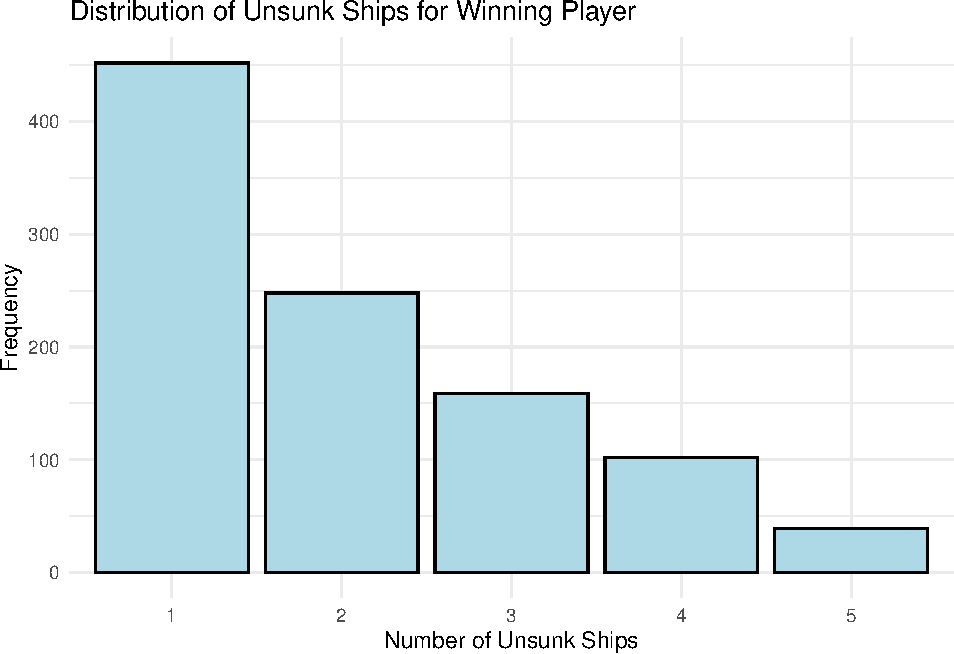
\includegraphics[keepaspectratio]{005707861_stats102a_midterm_files/figure-latex/unnamed-chunk-24-1.pdf}}

\subsubsection{The distribution of the number of unsunk ships the
winning player had remaining is
right-skewed.}\label{the-distribution-of-the-number-of-unsunk-ships-the-winning-player-had-remaining-is-right-skewed.-2}

\begin{Shaded}
\begin{Highlighting}[]
\CommentTok{\# d)}
\NormalTok{hits\_lp }\OtherTok{\textless{}{-}} \FunctionTok{sapply}\NormalTok{(}\DecValTok{1}\SpecialCharTok{:}\DecValTok{1000}\NormalTok{, }\ControlFlowTok{function}\NormalTok{ (i) \{}
\NormalTok{  winner }\OtherTok{\textless{}{-}} \FunctionTok{ifelse}\NormalTok{(}\FunctionTok{nrow}\NormalTok{(smart\_vs\_naive[[}\DecValTok{2}\NormalTok{, i]]}\SpecialCharTok{$}\NormalTok{history) }\SpecialCharTok{\%\%} \DecValTok{2}\NormalTok{, }\DecValTok{1}\NormalTok{, }\DecValTok{2}\NormalTok{) }\CommentTok{\# 1 or 2}
  \FunctionTok{sum}\NormalTok{(}\FunctionTok{sapply}\NormalTok{(smart\_vs\_naive[[}\DecValTok{2}\NormalTok{, i]]}\SpecialCharTok{$}\NormalTok{fleets[[winner]]}\SpecialCharTok{$}\NormalTok{ships, }\ControlFlowTok{function}\NormalTok{(comp) \{}
    \FunctionTok{sum}\NormalTok{(comp}\SpecialCharTok{$}\NormalTok{hits)}
\NormalTok{  \}))}
\NormalTok{\})}

\NormalTok{hits\_lp\_df }\OtherTok{\textless{}{-}} \FunctionTok{data.frame}\NormalTok{(hits\_lp)}

\CommentTok{\# Plot the distribution using ggplot2}
\FunctionTok{ggplot}\NormalTok{(hits\_lp\_df, }\FunctionTok{aes}\NormalTok{(}\AttributeTok{x =} \FunctionTok{factor}\NormalTok{(hits\_lp))) }\SpecialCharTok{+}
  \FunctionTok{geom\_bar}\NormalTok{(}\AttributeTok{fill =} \StringTok{"lightblue"}\NormalTok{, }\AttributeTok{color =} \StringTok{"black"}\NormalTok{) }\SpecialCharTok{+}
  \FunctionTok{labs}\NormalTok{(}\AttributeTok{title =} \StringTok{"Distribution of Hits Losing Player Made"}\NormalTok{, }
       \AttributeTok{x =} \StringTok{"Number of Hits"}\NormalTok{, }
       \AttributeTok{y =} \StringTok{"Frequency"}\NormalTok{) }\SpecialCharTok{+}
  \FunctionTok{theme\_minimal}\NormalTok{()}
\end{Highlighting}
\end{Shaded}

\pandocbounded{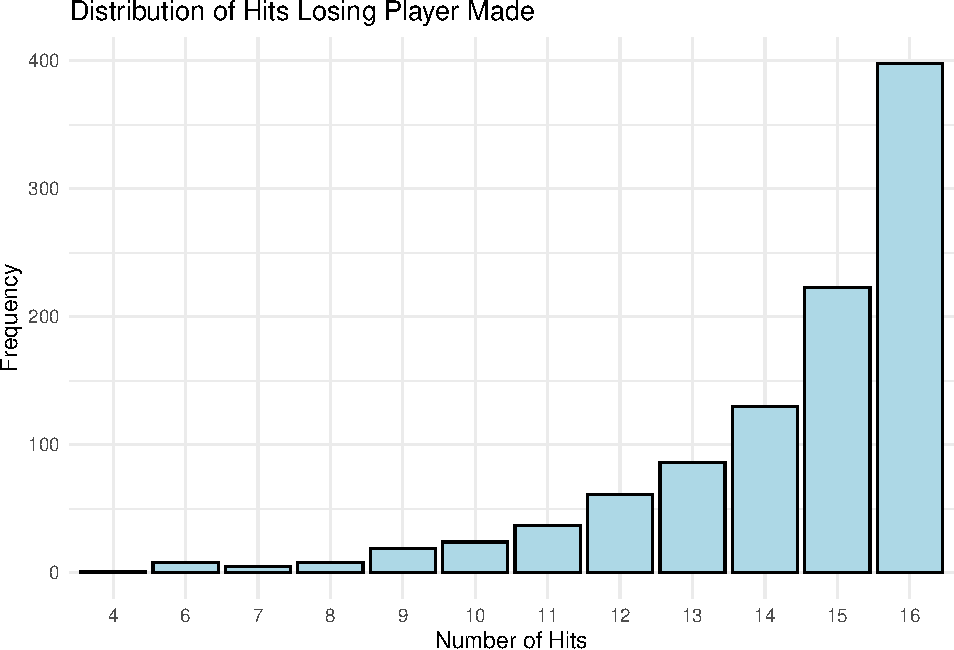
\includegraphics[keepaspectratio]{005707861_stats102a_midterm_files/figure-latex/unnamed-chunk-25-1.pdf}}

\subsubsection{The distribution of the number of hits the losing player
made is left-skewed with a minimum of 4 and maximum of
16.}\label{the-distribution-of-the-number-of-hits-the-losing-player-made-is-left-skewed-with-a-minimum-of-4-and-maximum-of-16.-1}

\begin{Shaded}
\begin{Highlighting}[]
\CommentTok{\# e)}
\NormalTok{patrol\_boats\_lost }\OtherTok{\textless{}{-}} \FunctionTok{sum}\NormalTok{(}\FunctionTok{sapply}\NormalTok{(}\DecValTok{1}\SpecialCharTok{:}\DecValTok{1000}\NormalTok{, }\ControlFlowTok{function}\NormalTok{ (i) \{}
\NormalTok{  winner }\OtherTok{\textless{}{-}} \FunctionTok{ifelse}\NormalTok{(}\FunctionTok{nrow}\NormalTok{(smart\_vs\_naive[[}\DecValTok{2}\NormalTok{, i]]}\SpecialCharTok{$}\NormalTok{history) }\SpecialCharTok{\%\%} \DecValTok{2}\NormalTok{, }\DecValTok{1}\NormalTok{, }\DecValTok{2}\NormalTok{) }\CommentTok{\# 1 or 2}
\NormalTok{  smart\_vs\_naive[[}\DecValTok{2}\NormalTok{, i]]}\SpecialCharTok{$}\NormalTok{fleets[[winner]]}\SpecialCharTok{$}\NormalTok{ships[[}\DecValTok{5}\NormalTok{]]}\SpecialCharTok{$}\NormalTok{sunk}
\NormalTok{\}))}

\NormalTok{(prop\_patrol\_boats\_lost }\OtherTok{\textless{}{-}}\NormalTok{ patrol\_boats\_lost }\SpecialCharTok{/} \DecValTok{1000}\NormalTok{)}
\end{Highlighting}
\end{Shaded}

\begin{verbatim}
## [1] 0.702
\end{verbatim}

\subsubsection{The proportion of games in which the winner lost their
Patrol Boat is
0.702.}\label{the-proportion-of-games-in-which-the-winner-lost-their-patrol-boat-is-0.702.}

\begin{Shaded}
\begin{Highlighting}[]
\CommentTok{\# f)}
\NormalTok{last\_ship\_patrol }\OtherTok{\textless{}{-}} \FunctionTok{sum}\NormalTok{(}\FunctionTok{sapply}\NormalTok{(}\DecValTok{1}\SpecialCharTok{:}\DecValTok{1000}\NormalTok{, }\ControlFlowTok{function}\NormalTok{ (i) \{}
\NormalTok{  comp }\OtherTok{\textless{}{-}}\NormalTok{ smart\_vs\_naive[[}\DecValTok{2}\NormalTok{, i]]}
\NormalTok{  winner }\OtherTok{\textless{}{-}} \FunctionTok{ifelse}\NormalTok{(}\FunctionTok{nrow}\NormalTok{(comp}\SpecialCharTok{$}\NormalTok{history) }\SpecialCharTok{\%\%} \DecValTok{2}\NormalTok{, }\DecValTok{1}\NormalTok{, }\DecValTok{2}\NormalTok{) }\CommentTok{\# 1 or 2}
\NormalTok{  patrol\_boat\_position }\OtherTok{\textless{}{-}}
\NormalTok{    comp}\SpecialCharTok{$}\NormalTok{fleets[[}\FunctionTok{ifelse}\NormalTok{(winner }\SpecialCharTok{==} \DecValTok{1}\NormalTok{, }\DecValTok{2}\NormalTok{, }\DecValTok{1}\NormalTok{)]]}\SpecialCharTok{$}\NormalTok{ships[[}\DecValTok{5}\NormalTok{]]}\SpecialCharTok{$}\NormalTok{position}
\NormalTok{  last\_target }\OtherTok{\textless{}{-}}\NormalTok{ comp}\SpecialCharTok{$}\NormalTok{history }\SpecialCharTok{\%\textgreater{}\%} \FunctionTok{pull}\NormalTok{(target) }\SpecialCharTok{\%\textgreater{}\%} \FunctionTok{tail}\NormalTok{(}\DecValTok{1}\NormalTok{)}
\NormalTok{  last\_target }\SpecialCharTok{\%in\%}\NormalTok{ patrol\_boat\_position}
\NormalTok{\}))}

\NormalTok{(prop\_last\_ship\_patrol }\OtherTok{\textless{}{-}}\NormalTok{ last\_ship\_patrol }\SpecialCharTok{/} \DecValTok{1000}\NormalTok{)}
\end{Highlighting}
\end{Shaded}

\begin{verbatim}
## [1] 0.181
\end{verbatim}

\subsubsection{The proportion of games in which the last ship of the
losing player is their Patrol Boat is
0.181.}\label{the-proportion-of-games-in-which-the-last-ship-of-the-losing-player-is-their-patrol-boat-is-0.181.}

\begin{Shaded}
\begin{Highlighting}[]
\CommentTok{\# smart(strength = 9) vs smart(strength = 9)}

\CommentTok{\# a)}
\FunctionTok{min}\NormalTok{(}\FunctionTok{sapply}\NormalTok{(smart\_vs\_smart[}\DecValTok{2}\NormalTok{, ], }\ControlFlowTok{function}\NormalTok{(comp) }\FunctionTok{nrow}\NormalTok{(comp}\SpecialCharTok{$}\NormalTok{history)))}
\end{Highlighting}
\end{Shaded}

\begin{verbatim}
## [1] 77
\end{verbatim}

\subsubsection{In an ideal scenario the player would win in 17 turns (if
they hit a ship every time they go). Going back and forth, the
theorectical minimum is 33 turns if that same player goes first. The
actual minimum of 77 is higher than the theoretical
minimum.}\label{in-an-ideal-scenario-the-player-would-win-in-17-turns-if-they-hit-a-ship-every-time-they-go.-going-back-and-forth-the-theorectical-minimum-is-33-turns-if-that-same-player-goes-first.-the-actual-minimum-of-77-is-higher-than-the-theoretical-minimum.}

\begin{Shaded}
\begin{Highlighting}[]
\CommentTok{\# b)}
\FunctionTok{max}\NormalTok{(}\FunctionTok{sapply}\NormalTok{(smart\_vs\_smart[}\DecValTok{2}\NormalTok{, ], }\ControlFlowTok{function}\NormalTok{(comp) }\FunctionTok{nrow}\NormalTok{(comp}\SpecialCharTok{$}\NormalTok{history)))}
\end{Highlighting}
\end{Shaded}

\begin{verbatim}
## [1] 199
\end{verbatim}

\subsubsection{In the worst case scenario the player would win in 50
turns (if they go first). Going back and forth, the theorectical maximum
is 199 turns if that same player goes first. The actual maximum of 199
is equal to the theoretical
minimum.}\label{in-the-worst-case-scenario-the-player-would-win-in-50-turns-if-they-go-first.-going-back-and-forth-the-theorectical-maximum-is-199-turns-if-that-same-player-goes-first.-the-actual-maximum-of-199-is-equal-to-the-theoretical-minimum.-2}

\begin{Shaded}
\begin{Highlighting}[]
\CommentTok{\# c)}
\NormalTok{unsunk\_ships }\OtherTok{\textless{}{-}} \FunctionTok{sapply}\NormalTok{(}\DecValTok{1}\SpecialCharTok{:}\DecValTok{1000}\NormalTok{, }\ControlFlowTok{function}\NormalTok{ (i) \{}
\NormalTok{  winner }\OtherTok{\textless{}{-}} \FunctionTok{ifelse}\NormalTok{(}\FunctionTok{nrow}\NormalTok{(smart\_vs\_smart[[}\DecValTok{2}\NormalTok{, i]]}\SpecialCharTok{$}\NormalTok{history) }\SpecialCharTok{\%\%} \DecValTok{2}\NormalTok{, }\DecValTok{1}\NormalTok{, }\DecValTok{2}\NormalTok{) }\CommentTok{\# 1 or 2}
  \FunctionTok{sum}\NormalTok{(}\FunctionTok{sapply}\NormalTok{(smart\_vs\_smart[[}\DecValTok{2}\NormalTok{, i]]}\SpecialCharTok{$}\NormalTok{fleets[[winner]]}\SpecialCharTok{$}\NormalTok{ships, }\ControlFlowTok{function}\NormalTok{(comp) \{}
    \SpecialCharTok{!}\NormalTok{comp}\SpecialCharTok{$}\NormalTok{sunk}
\NormalTok{  \}))}
\NormalTok{\})}

\NormalTok{unsunk\_ships\_df }\OtherTok{\textless{}{-}} \FunctionTok{data.frame}\NormalTok{(unsunk\_ships)}

\CommentTok{\# Plot the distribution using ggplot2}
\FunctionTok{ggplot}\NormalTok{(unsunk\_ships\_df, }\FunctionTok{aes}\NormalTok{(}\AttributeTok{x =} \FunctionTok{factor}\NormalTok{(unsunk\_ships))) }\SpecialCharTok{+}
  \FunctionTok{geom\_bar}\NormalTok{(}\AttributeTok{fill =} \StringTok{"lightblue"}\NormalTok{, }\AttributeTok{color =} \StringTok{"black"}\NormalTok{) }\SpecialCharTok{+}
  \FunctionTok{labs}\NormalTok{(}\AttributeTok{title =} \StringTok{"Distribution of Unsunk Ships for Winning Player"}\NormalTok{, }
       \AttributeTok{x =} \StringTok{"Number of Unsunk Ships"}\NormalTok{, }
       \AttributeTok{y =} \StringTok{"Frequency"}\NormalTok{) }\SpecialCharTok{+}
  \FunctionTok{theme\_minimal}\NormalTok{()}
\end{Highlighting}
\end{Shaded}

\pandocbounded{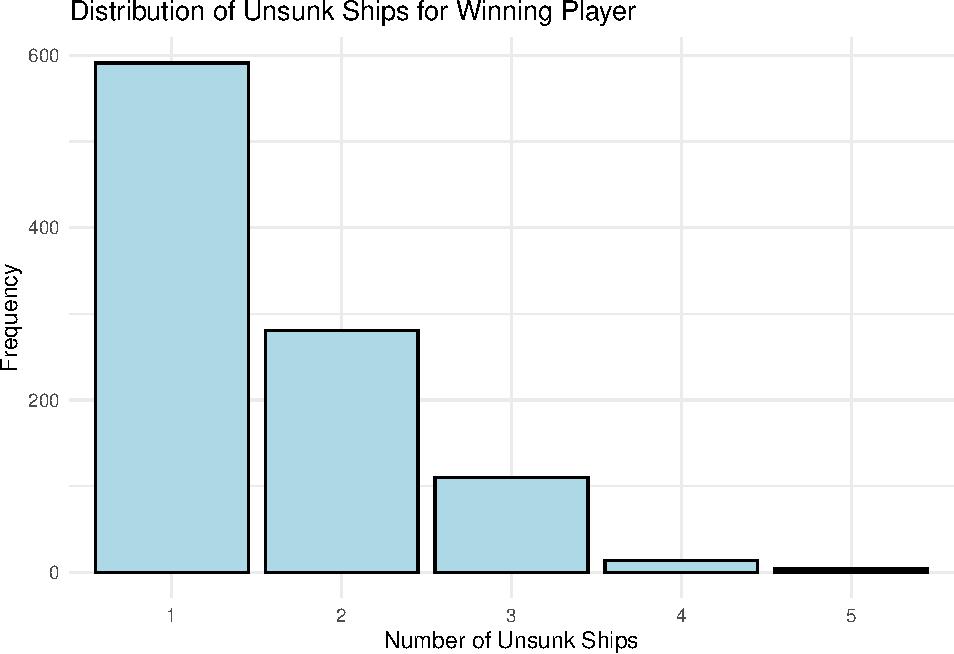
\includegraphics[keepaspectratio]{005707861_stats102a_midterm_files/figure-latex/unnamed-chunk-30-1.pdf}}

\subsubsection{The distribution of the number of unsunk ships the
winning player had remaining is
right-skewed.}\label{the-distribution-of-the-number-of-unsunk-ships-the-winning-player-had-remaining-is-right-skewed.-3}

\begin{Shaded}
\begin{Highlighting}[]
\CommentTok{\# d)}
\NormalTok{hits\_lp }\OtherTok{\textless{}{-}} \FunctionTok{sapply}\NormalTok{(}\DecValTok{1}\SpecialCharTok{:}\DecValTok{1000}\NormalTok{, }\ControlFlowTok{function}\NormalTok{ (i) \{}
\NormalTok{  winner }\OtherTok{\textless{}{-}} \FunctionTok{ifelse}\NormalTok{(}\FunctionTok{nrow}\NormalTok{(smart\_vs\_smart[[}\DecValTok{2}\NormalTok{, i]]}\SpecialCharTok{$}\NormalTok{history) }\SpecialCharTok{\%\%} \DecValTok{2}\NormalTok{, }\DecValTok{1}\NormalTok{, }\DecValTok{2}\NormalTok{) }\CommentTok{\# 1 or 2}
  \FunctionTok{sum}\NormalTok{(}\FunctionTok{sapply}\NormalTok{(smart\_vs\_smart[[}\DecValTok{2}\NormalTok{, i]]}\SpecialCharTok{$}\NormalTok{fleets[[winner]]}\SpecialCharTok{$}\NormalTok{ships, }\ControlFlowTok{function}\NormalTok{(comp) \{}
    \FunctionTok{sum}\NormalTok{(comp}\SpecialCharTok{$}\NormalTok{hits)}
\NormalTok{  \}))}
\NormalTok{\})}

\NormalTok{hits\_lp\_df }\OtherTok{\textless{}{-}} \FunctionTok{data.frame}\NormalTok{(hits\_lp)}

\CommentTok{\# Plot the distribution using ggplot2}
\FunctionTok{ggplot}\NormalTok{(hits\_lp\_df, }\FunctionTok{aes}\NormalTok{(}\AttributeTok{x =} \FunctionTok{factor}\NormalTok{(hits\_lp))) }\SpecialCharTok{+}
  \FunctionTok{geom\_bar}\NormalTok{(}\AttributeTok{fill =} \StringTok{"lightblue"}\NormalTok{, }\AttributeTok{color =} \StringTok{"black"}\NormalTok{) }\SpecialCharTok{+}
  \FunctionTok{labs}\NormalTok{(}\AttributeTok{title =} \StringTok{"Distribution of Hits Losing Player Made"}\NormalTok{, }
       \AttributeTok{x =} \StringTok{"Number of Hits"}\NormalTok{, }
       \AttributeTok{y =} \StringTok{"Frequency"}\NormalTok{) }\SpecialCharTok{+}
  \FunctionTok{theme\_minimal}\NormalTok{()}
\end{Highlighting}
\end{Shaded}

\pandocbounded{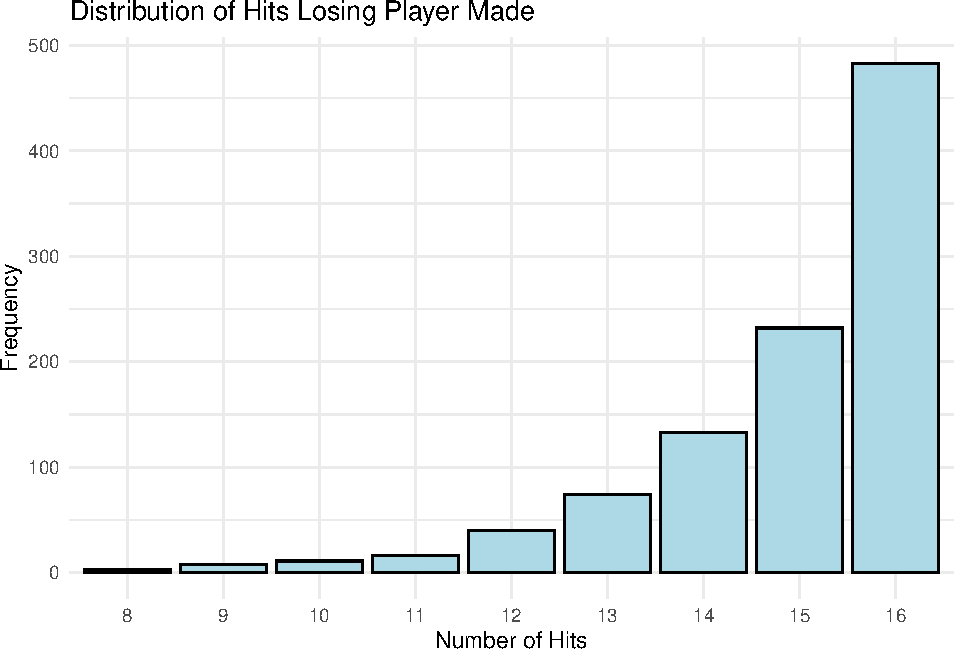
\includegraphics[keepaspectratio]{005707861_stats102a_midterm_files/figure-latex/unnamed-chunk-31-1.pdf}}

\subsubsection{The distribution of the number of hits the losing player
made is left-skewed with a minimum of 8 and maximum of
16.}\label{the-distribution-of-the-number-of-hits-the-losing-player-made-is-left-skewed-with-a-minimum-of-8-and-maximum-of-16.-1}

\begin{Shaded}
\begin{Highlighting}[]
\CommentTok{\# e)}
\NormalTok{patrol\_boats\_lost }\OtherTok{\textless{}{-}} \FunctionTok{sum}\NormalTok{(}\FunctionTok{sapply}\NormalTok{(}\DecValTok{1}\SpecialCharTok{:}\DecValTok{1000}\NormalTok{, }\ControlFlowTok{function}\NormalTok{ (i) \{}
\NormalTok{  winner }\OtherTok{\textless{}{-}} \FunctionTok{ifelse}\NormalTok{(}\FunctionTok{nrow}\NormalTok{(smart\_vs\_smart[[}\DecValTok{2}\NormalTok{, i]]}\SpecialCharTok{$}\NormalTok{history) }\SpecialCharTok{\%\%} \DecValTok{2}\NormalTok{, }\DecValTok{1}\NormalTok{, }\DecValTok{2}\NormalTok{) }\CommentTok{\# 1 or 2}
\NormalTok{  smart\_vs\_smart[[}\DecValTok{2}\NormalTok{, i]]}\SpecialCharTok{$}\NormalTok{fleets[[winner]]}\SpecialCharTok{$}\NormalTok{ships[[}\DecValTok{5}\NormalTok{]]}\SpecialCharTok{$}\NormalTok{sunk}
\NormalTok{\}))}

\NormalTok{(prop\_patrol\_boats\_lost }\OtherTok{\textless{}{-}}\NormalTok{ patrol\_boats\_lost }\SpecialCharTok{/} \DecValTok{1000}\NormalTok{)}
\end{Highlighting}
\end{Shaded}

\begin{verbatim}
## [1] 0.731
\end{verbatim}

\subsubsection{The proportion of games in which the winner lost their
Patrol Boat is
0.731.}\label{the-proportion-of-games-in-which-the-winner-lost-their-patrol-boat-is-0.731.}

\begin{Shaded}
\begin{Highlighting}[]
\CommentTok{\# f)}
\NormalTok{last\_ship\_patrol }\OtherTok{\textless{}{-}} \FunctionTok{sum}\NormalTok{(}\FunctionTok{sapply}\NormalTok{(}\DecValTok{1}\SpecialCharTok{:}\DecValTok{1000}\NormalTok{, }\ControlFlowTok{function}\NormalTok{ (i) \{}
\NormalTok{  comp }\OtherTok{\textless{}{-}}\NormalTok{ smart\_vs\_smart[[}\DecValTok{2}\NormalTok{, i]]}
\NormalTok{  winner }\OtherTok{\textless{}{-}} \FunctionTok{ifelse}\NormalTok{(}\FunctionTok{nrow}\NormalTok{(comp}\SpecialCharTok{$}\NormalTok{history) }\SpecialCharTok{\%\%} \DecValTok{2}\NormalTok{, }\DecValTok{1}\NormalTok{, }\DecValTok{2}\NormalTok{) }\CommentTok{\# 1 or 2}
\NormalTok{  patrol\_boat\_position }\OtherTok{\textless{}{-}}
\NormalTok{    comp}\SpecialCharTok{$}\NormalTok{fleets[[}\FunctionTok{ifelse}\NormalTok{(winner }\SpecialCharTok{==} \DecValTok{1}\NormalTok{, }\DecValTok{2}\NormalTok{, }\DecValTok{1}\NormalTok{)]]}\SpecialCharTok{$}\NormalTok{ships[[}\DecValTok{5}\NormalTok{]]}\SpecialCharTok{$}\NormalTok{position}
\NormalTok{  last\_target }\OtherTok{\textless{}{-}}\NormalTok{ comp}\SpecialCharTok{$}\NormalTok{history }\SpecialCharTok{\%\textgreater{}\%} \FunctionTok{pull}\NormalTok{(target) }\SpecialCharTok{\%\textgreater{}\%} \FunctionTok{tail}\NormalTok{(}\DecValTok{1}\NormalTok{)}
\NormalTok{  last\_target }\SpecialCharTok{\%in\%}\NormalTok{ patrol\_boat\_position}
\NormalTok{\}))}

\NormalTok{(prop\_last\_ship\_patrol }\OtherTok{\textless{}{-}}\NormalTok{ last\_ship\_patrol }\SpecialCharTok{/} \DecValTok{1000}\NormalTok{)}
\end{Highlighting}
\end{Shaded}

\begin{verbatim}
## [1] 0.185
\end{verbatim}

\subsubsection{The proportion of games in which the last ship of the
losing player is their Patrol Boat is
0.185.}\label{the-proportion-of-games-in-which-the-last-ship-of-the-losing-player-is-their-patrol-boat-is-0.185.}

Also answer the following questions:

\begin{enumerate}[label=\alph*)]
\setcounter{enumi}{6}
\item Make a two-way relative frequency table of the proportion of times Player 1 (whoever goes fist) wins.
\item Test the hypothesis that order of play is not a statistically significant factor in determining who wins. Use a 5\% significance level, and interpret the $p$-value.
\item Test the hypothesis that the type of AI player is not a statistically significant factor in determining who wins. Use a 5\% significance level, and interpret the $p$-value.
\end{enumerate}

\begin{Shaded}
\begin{Highlighting}[]
\CommentTok{\# g)}

\NormalTok{prop\_first\_player\_naive\_vs\_naive }\OtherTok{\textless{}{-}} \FunctionTok{sum}\NormalTok{(}\FunctionTok{sapply}\NormalTok{(}\DecValTok{1}\SpecialCharTok{:}\DecValTok{1000}\NormalTok{, }\ControlFlowTok{function}\NormalTok{(i) \{}
  \FunctionTok{nrow}\NormalTok{(naive\_vs\_naive[[}\DecValTok{2}\NormalTok{, i]]}\SpecialCharTok{$}\NormalTok{history) }\SpecialCharTok{\%\%} \DecValTok{2} \SpecialCharTok{==} \DecValTok{1}
\NormalTok{\})) }\SpecialCharTok{/} \DecValTok{1000}

\NormalTok{prop\_first\_player\_naive\_vs\_smart }\OtherTok{\textless{}{-}} \FunctionTok{sum}\NormalTok{(}\FunctionTok{sapply}\NormalTok{(}\DecValTok{1}\SpecialCharTok{:}\DecValTok{1000}\NormalTok{, }\ControlFlowTok{function}\NormalTok{(i) \{}
  \FunctionTok{nrow}\NormalTok{(naive\_vs\_smart[[}\DecValTok{2}\NormalTok{, i]]}\SpecialCharTok{$}\NormalTok{history) }\SpecialCharTok{\%\%} \DecValTok{2} \SpecialCharTok{==} \DecValTok{1}
\NormalTok{\})) }\SpecialCharTok{/} \DecValTok{1000}

\NormalTok{prop\_first\_player\_smart\_vs\_naive }\OtherTok{\textless{}{-}} \FunctionTok{sum}\NormalTok{(}\FunctionTok{sapply}\NormalTok{(}\DecValTok{1}\SpecialCharTok{:}\DecValTok{1000}\NormalTok{, }\ControlFlowTok{function}\NormalTok{(i) \{}
  \FunctionTok{nrow}\NormalTok{(smart\_vs\_naive[[}\DecValTok{2}\NormalTok{, i]]}\SpecialCharTok{$}\NormalTok{history) }\SpecialCharTok{\%\%} \DecValTok{2} \SpecialCharTok{==} \DecValTok{1}
\NormalTok{\})) }\SpecialCharTok{/} \DecValTok{1000}

\NormalTok{prop\_first\_player\_smart\_vs\_smart }\OtherTok{\textless{}{-}} \FunctionTok{sum}\NormalTok{(}\FunctionTok{sapply}\NormalTok{(}\DecValTok{1}\SpecialCharTok{:}\DecValTok{1000}\NormalTok{, }\ControlFlowTok{function}\NormalTok{(i) \{}
  \FunctionTok{nrow}\NormalTok{(smart\_vs\_smart[[}\DecValTok{2}\NormalTok{, i]]}\SpecialCharTok{$}\NormalTok{history) }\SpecialCharTok{\%\%} \DecValTok{2} \SpecialCharTok{==} \DecValTok{1}
\NormalTok{\})) }\SpecialCharTok{/} \DecValTok{1000}
\end{Highlighting}
\end{Shaded}

\begin{longtable}[]{@{}lll@{}}
\toprule\noalign{}
& Player 2 Naive & Player 2 Smart \\
\midrule\noalign{}
\endhead
\bottomrule\noalign{}
\endlastfoot
Player 1 Naive & 0.571 & 0.29 \\
Player 1 Smart & 0.78 & 0.514 \\
\end{longtable}

\begin{Shaded}
\begin{Highlighting}[]
\CommentTok{\# h) }
\NormalTok{total\_wins\_player1 }\OtherTok{\textless{}{-}}\NormalTok{ (prop\_first\_player\_naive\_vs\_naive }\SpecialCharTok{*} \DecValTok{1000}\NormalTok{) }\SpecialCharTok{+}
\NormalTok{                      (prop\_first\_player\_naive\_vs\_smart }\SpecialCharTok{*} \DecValTok{1000}\NormalTok{) }\SpecialCharTok{+}
\NormalTok{                      (prop\_first\_player\_smart\_vs\_naive }\SpecialCharTok{*} \DecValTok{1000}\NormalTok{) }\SpecialCharTok{+}
\NormalTok{                      (prop\_first\_player\_smart\_vs\_smart }\SpecialCharTok{*} \DecValTok{1000}\NormalTok{)}

\CommentTok{\# perform one{-}sample proportion test}
\NormalTok{test\_result }\OtherTok{\textless{}{-}} \FunctionTok{prop.test}\NormalTok{(}\AttributeTok{x =}\NormalTok{ total\_wins\_player1, }\AttributeTok{n =} \DecValTok{4000}\NormalTok{, }\AttributeTok{p =} \FloatTok{0.5}\NormalTok{, }\AttributeTok{alternative =} \StringTok{"two.sided"}\NormalTok{)}

\CommentTok{\# extract p{-}value from test result}
\NormalTok{(p\_value }\OtherTok{\textless{}{-}}\NormalTok{ test\_result}\SpecialCharTok{$}\NormalTok{p.value)}
\end{Highlighting}
\end{Shaded}

\begin{verbatim}
## [1] 1.030521e-06
\end{verbatim}

Since the p-value \ensuremath{1.0305209\times 10^{-6}} is much smaller
than \(\alpha=0.05\), we reject the null hypothesis and conclude that
the order of play is a statistically significant factor in determining
who wins. The evidence is sufficient to support the alternative
hypothesis that the probability that Player 1 wins is not 0.50.

\begin{Shaded}
\begin{Highlighting}[]
\CommentTok{\# i) }
\NormalTok{total\_smart\_wins\_naive\_vs\_smart }\OtherTok{\textless{}{-}} \FunctionTok{sum}\NormalTok{(}\FunctionTok{sapply}\NormalTok{(}\DecValTok{1}\SpecialCharTok{:}\DecValTok{1000}\NormalTok{, }\ControlFlowTok{function}\NormalTok{(i) \{}
  \FunctionTok{nrow}\NormalTok{(naive\_vs\_smart[[}\DecValTok{2}\NormalTok{, i]]}\SpecialCharTok{$}\NormalTok{history) }\SpecialCharTok{\%\%} \DecValTok{2} \SpecialCharTok{==} \DecValTok{0} \CommentTok{\# since smart is player 2 }
\NormalTok{\})) }

\NormalTok{total\_smart\_wins\_smart\_vs\_naive }\OtherTok{\textless{}{-}} \FunctionTok{sum}\NormalTok{(}\FunctionTok{sapply}\NormalTok{(}\DecValTok{1}\SpecialCharTok{:}\DecValTok{1000}\NormalTok{, }\ControlFlowTok{function}\NormalTok{(i) \{}
  \FunctionTok{nrow}\NormalTok{(smart\_vs\_naive[[}\DecValTok{2}\NormalTok{, i]]}\SpecialCharTok{$}\NormalTok{history) }\SpecialCharTok{\%\%} \DecValTok{2} \SpecialCharTok{==} \DecValTok{1} \CommentTok{\# since smart is player 1}
\NormalTok{\}))}

\NormalTok{total\_smart\_wins }\OtherTok{\textless{}{-}}\NormalTok{ total\_smart\_wins\_naive\_vs\_smart }\SpecialCharTok{+}\NormalTok{ total\_smart\_wins\_smart\_vs\_naive}
\NormalTok{total\_naive\_wins }\OtherTok{\textless{}{-}} \DecValTok{2000} \SpecialCharTok{{-}}\NormalTok{ total\_smart\_wins}

\NormalTok{test\_result }\OtherTok{\textless{}{-}} \FunctionTok{prop.test}\NormalTok{(}\AttributeTok{x =}\NormalTok{ total\_smart\_wins, }\AttributeTok{n =} \DecValTok{2000}\NormalTok{, }\AttributeTok{p =} \FloatTok{0.5}\NormalTok{, }\AttributeTok{alternative =} \StringTok{"two.sided"}\NormalTok{)}

\NormalTok{(p\_value }\OtherTok{\textless{}{-}}\NormalTok{ test\_result}\SpecialCharTok{$}\NormalTok{p.value)}
\end{Highlighting}
\end{Shaded}

\begin{verbatim}
## [1] 3.157631e-106
\end{verbatim}

Since the p-value \ensuremath{3.1576313\times 10^{-106}} is much smaller
than \(\alpha=0.05\), we reject the null hypothesis and conclude that
the type of AI player is a statistically significant factor in
determining who wins. The evidence is sufficient to support the
alternative hypothesis that the probability of the naive player winning
is not equal to the probability of the smart player winning.

\subsubsection{C) Handicapped Games}\label{c-handicapped-games}

If you wrote your functions as specified in a general enough way, it
should be possible to conduct a game between two different fleets on two
different oceans. Experiment with changing the setup of the game to give
one player an advantage over another. Perhaps you simply give one player
a \(9\times 9\) board to hide their ships in and you give the other
player an \(11\times 11\) board to hide in. Or you trade one player's
Patrol Boat for the other player's submarine.

Try \emph{at least} \textbf{three different} handicaps in favor of the
naive AI against your smart AI with the goal of making it a fair game
between the two.

Run 100,000 simulations and provide some summary statistics for each set
of simulations. Don't worry if it's not exactly fair, even with the
handicap, but it should change your results in the right direction.

\subsubsection{Handicap 1 - Board Size: Give smart player a 8 x 8 board
to hide their ships and naive player 11 x 11 board to hide their ships,
so smart player may take longer to hit and sink the naive player's
ships, and naive player has better chance of sinking all of smart
player's ships before smart player gets to sink all
theirs.}\label{handicap-1---board-size-give-smart-player-a-8-x-8-board-to-hide-their-ships-and-naive-player-11-x-11-board-to-hide-their-ships-so-smart-player-may-take-longer-to-hit-and-sink-the-naive-players-ships-and-naive-player-has-better-chance-of-sinking-all-of-smart-players-ships-before-smart-player-gets-to-sink-all-theirs.}

\begin{Shaded}
\begin{Highlighting}[]
\CommentTok{\# first player naive, second player smart}
\CommentTok{\# set.seed(123)}
\CommentTok{\# handicap\_board\_size \textless{}{-} replicate(1000, play\_bs(players = c("ai\_005707861", "ai\_005707861"), }
\CommentTok{\#                                                strengths = c(0, 9), oceans = list(c(11, 11), c(8, 8))))}
\CommentTok{\# save(handicap\_board\_size, file = "handicap\_board\_size.RData")}
\FunctionTok{load}\NormalTok{(}\StringTok{"handicap\_board\_size.RData"}\NormalTok{)}

\CommentTok{\# summary statistics}

\NormalTok{summary\_handicap }\OtherTok{\textless{}{-}} \ControlFlowTok{function}\NormalTok{(handicap) \{}
\NormalTok{  min\_turns }\OtherTok{\textless{}{-}} \FunctionTok{min}\NormalTok{(}\FunctionTok{sapply}\NormalTok{(handicap[}\DecValTok{2}\NormalTok{, ], }\ControlFlowTok{function}\NormalTok{(comp) }\FunctionTok{nrow}\NormalTok{(comp}\SpecialCharTok{$}\NormalTok{history)))}
\NormalTok{  max\_turns }\OtherTok{\textless{}{-}} \FunctionTok{max}\NormalTok{(}\FunctionTok{sapply}\NormalTok{(handicap[}\DecValTok{2}\NormalTok{, ], }\ControlFlowTok{function}\NormalTok{(comp) }\FunctionTok{nrow}\NormalTok{(comp}\SpecialCharTok{$}\NormalTok{history)))}
\NormalTok{  avg\_turns }\OtherTok{\textless{}{-}} \FunctionTok{mean}\NormalTok{(}\FunctionTok{sapply}\NormalTok{(handicap[}\DecValTok{2}\NormalTok{, ], }\ControlFlowTok{function}\NormalTok{(comp) }\FunctionTok{nrow}\NormalTok{(comp}\SpecialCharTok{$}\NormalTok{history)))}
\NormalTok{  avg\_unsunk\_ships }\OtherTok{\textless{}{-}} \FunctionTok{mean}\NormalTok{(}\FunctionTok{sapply}\NormalTok{(}\DecValTok{1}\SpecialCharTok{:}\DecValTok{1000}\NormalTok{, }\ControlFlowTok{function}\NormalTok{ (i) \{}
\NormalTok{    winner }\OtherTok{\textless{}{-}} \FunctionTok{ifelse}\NormalTok{(}\FunctionTok{nrow}\NormalTok{(handicap[[}\DecValTok{2}\NormalTok{, i]]}\SpecialCharTok{$}\NormalTok{history) }\SpecialCharTok{\%\%} \DecValTok{2}\NormalTok{, }\DecValTok{1}\NormalTok{, }\DecValTok{2}\NormalTok{) }\CommentTok{\# 1 or 2}
    \FunctionTok{sum}\NormalTok{(}\FunctionTok{sapply}\NormalTok{(handicap[[}\DecValTok{2}\NormalTok{, i]]}\SpecialCharTok{$}\NormalTok{fleets[[winner]]}\SpecialCharTok{$}\NormalTok{ships, }\ControlFlowTok{function}\NormalTok{(comp) \{}
      \SpecialCharTok{!}\NormalTok{comp}\SpecialCharTok{$}\NormalTok{sunk}
\NormalTok{    \}))}
\NormalTok{  \}))}
\NormalTok{  prop\_naive\_wins\_handicap }\OtherTok{\textless{}{-}} \FunctionTok{sum}\NormalTok{(}\FunctionTok{sapply}\NormalTok{(}\DecValTok{1}\SpecialCharTok{:}\DecValTok{1000}\NormalTok{, }\ControlFlowTok{function}\NormalTok{(i) \{}
    \FunctionTok{nrow}\NormalTok{(handicap[[}\DecValTok{2}\NormalTok{, i]]}\SpecialCharTok{$}\NormalTok{history) }\SpecialCharTok{\%\%} \DecValTok{2} \SpecialCharTok{==} \DecValTok{1}
\NormalTok{  \})) }\SpecialCharTok{/} \DecValTok{1000}
\NormalTok{  out }\OtherTok{\textless{}{-}} \FunctionTok{c}\NormalTok{(min\_turns, max\_turns, avg\_turns, avg\_unsunk\_ships, prop\_naive\_wins\_handicap)}
  \FunctionTok{names}\NormalTok{(out) }\OtherTok{\textless{}{-}} \FunctionTok{c}\NormalTok{(}\StringTok{"minimum turns"}\NormalTok{, }\StringTok{"max\_turns"}\NormalTok{, }\StringTok{"avg\_turns"}\NormalTok{, }\StringTok{"avg\_unsunk\_ships"}\NormalTok{, }\StringTok{"naive\_win\_rate"}\NormalTok{)}
\NormalTok{  out}
\NormalTok{\}}

\FunctionTok{summary\_handicap}\NormalTok{(handicap\_board\_size)}
\end{Highlighting}
\end{Shaded}

\begin{verbatim}
##    minimum turns        max_turns        avg_turns avg_unsunk_ships 
##           92.000          127.000          121.775            2.563 
##   naive_win_rate 
##            0.981
\end{verbatim}

\subsubsection{Handicap 2 - Ship Size: Give smart player five patrol
boats and naive player five battleships, so that there are 10 (20 - 10)
less spots that naive has to hit to win the
game.}\label{handicap-2---ship-size-give-smart-player-five-patrol-boats-and-naive-player-five-battleships-so-that-there-are-10-20---10-less-spots-that-naive-has-to-hit-to-win-the-game.}

\begin{Shaded}
\begin{Highlighting}[]
\NormalTok{fleet\_size }\OtherTok{=} \FunctionTok{list}\NormalTok{(}\FunctionTok{list}\NormalTok{(}
  \FunctionTok{ship}\NormalTok{(}\StringTok{"Battleship"}\NormalTok{, }\DecValTok{4}\NormalTok{),}
  \FunctionTok{ship}\NormalTok{(}\StringTok{"Battleship"}\NormalTok{, }\DecValTok{4}\NormalTok{),}
  \FunctionTok{ship}\NormalTok{(}\StringTok{"Battleship"}\NormalTok{, }\DecValTok{4}\NormalTok{),}
  \FunctionTok{ship}\NormalTok{(}\StringTok{"Battleship"}\NormalTok{, }\DecValTok{4}\NormalTok{),}
  \FunctionTok{ship}\NormalTok{(}\StringTok{"Battleship"}\NormalTok{, }\DecValTok{4}\NormalTok{)}
\NormalTok{),}
\FunctionTok{list}\NormalTok{(}
  \FunctionTok{ship}\NormalTok{(}\StringTok{"Patrol Boat"}\NormalTok{, }\DecValTok{2}\NormalTok{),}
  \FunctionTok{ship}\NormalTok{(}\StringTok{"Patrol Boat"}\NormalTok{, }\DecValTok{2}\NormalTok{),}
  \FunctionTok{ship}\NormalTok{(}\StringTok{"Patrol Boat"}\NormalTok{, }\DecValTok{2}\NormalTok{),}
  \FunctionTok{ship}\NormalTok{(}\StringTok{"Patrol Boat"}\NormalTok{, }\DecValTok{2}\NormalTok{),}
  \FunctionTok{ship}\NormalTok{(}\StringTok{"Patrol Boat"}\NormalTok{, }\DecValTok{2}\NormalTok{)}
\NormalTok{))}
  
\CommentTok{\# handicap\_ship\_size \textless{}{-} replicate(1000, play\_bs(players = c("ai\_005707861", "ai\_005707861"), strengths = c(0, 9),}
\CommentTok{\#         fleet\_size = fleet\_size))}
\CommentTok{\# save(handicap\_ship\_size, file = "handicap\_ship\_size.RData")}
\FunctionTok{load}\NormalTok{(}\StringTok{"handicap\_ship\_size.RData"}\NormalTok{)}
\FunctionTok{summary\_handicap}\NormalTok{(handicap\_ship\_size)}
\end{Highlighting}
\end{Shaded}

\begin{verbatim}
##    minimum turns        max_turns        avg_turns avg_unsunk_ships 
##           76.000          199.000          169.974            1.639 
##   naive_win_rate 
##            0.444
\end{verbatim}

\subsubsection{Handicap 3 - Fleet Size: Give naive player 7 ships, and
smart player standard number - more ships may increase the chance for
the naive player to survive longer in the
game.}\label{handicap-3---fleet-size-give-naive-player-7-ships-and-smart-player-standard-number---more-ships-may-increase-the-chance-for-the-naive-player-to-survive-longer-in-the-game.}

\begin{Shaded}
\begin{Highlighting}[]
\NormalTok{fleet\_size }\OtherTok{=} \FunctionTok{list}\NormalTok{(}\FunctionTok{c}\NormalTok{(}\FunctionTok{default\_ships}\NormalTok{(), }\FunctionTok{list}\NormalTok{(}
  \FunctionTok{ship}\NormalTok{(}\StringTok{"Submarine"}\NormalTok{, }\DecValTok{3}\NormalTok{), }\FunctionTok{ship}\NormalTok{(}\StringTok{"Submarine"}\NormalTok{, }\DecValTok{3}\NormalTok{)}
\NormalTok{)),}
\FunctionTok{default\_ships}\NormalTok{())}

\CommentTok{\# handicap\_fleet\_size \textless{}{-} replicate(1000, play\_bs(players = c("ai\_005707861", "ai\_005707861"), strengths = c(0, 9), }
\CommentTok{\#         fleet\_size = fleet\_size))}
\CommentTok{\# save(handicap\_fleet\_size, file = "handicap\_fleet\_size.RData")}
\FunctionTok{load}\NormalTok{(}\StringTok{"handicap\_fleet\_size.RData"}\NormalTok{)}
\FunctionTok{summary\_handicap}\NormalTok{(handicap\_fleet\_size)}
\end{Highlighting}
\end{Shaded}

\begin{verbatim}
##    minimum turns        max_turns        avg_turns avg_unsunk_ships 
##           90.000          199.000          181.008            1.671 
##   naive_win_rate 
##            0.406
\end{verbatim}

\subsubsection{D) Extensions}\label{d-extensions}

\begin{enumerate}[label=\alph*)]
\item Describe in as much detail as possible, what you would need to change to implement the Salvo! variant of the game. (See rules.)
\item Identify at least two (2) ways you could modify or extend the game, other than the Salvo! variant, and describe in as much detail as possible what you would need to change to implement each of the extensions you identified. Do not implement these changes.
\end{enumerate}

\subsubsection{\texorpdfstring{a) In the Hasbro Salvo! variation, on
their turn a player targets five squares and marks their secondary
boards with white pegs. The opponent then annouces which shots were
hits, and if any were hits both the player and the opponent place red
pegs on the squares of their secondary and primary boards, respectively.
For the Salvo! variation, I would have to modify the while loop
iterating through turns. When prompting the human player for targets, I
would surround the \texttt{target\ \textless{}-\ human()} command with a
for loop to get 5 inputs and keep track of valid inputs in a vector to
make sure the user doesn't enter the same target multiple times. For the
\texttt{ai\_005707861.battleship()} function I would update memory with
a \texttt{last\_hit} vector and remove/add squares accordingly, and have
the AI in search mode (randomly choose targets) for any
\texttt{last\_hit} vectors with less than five squares, and for the
\texttt{last\_hit} elements go through and keep track of their
respective tried directions (e.g.~up, down, left, right) and successful
directions. So the \texttt{ai\_005707861.battleship()} would return a
list with two components: \texttt{targets}, a vector of five squares,
and \texttt{memory} where each component can have more than one element.
Back in the while loop in \texttt{play\_bs()}, I would also modify
\texttt{hit} to be a logical vector of length 5 and iterate through a
for loop to check if each of the current player's target was a hit or
miss, and update the players' ships and the game's history
accordingly.}{a) In the Hasbro Salvo! variation, on their turn a player targets five squares and marks their secondary boards with white pegs. The opponent then annouces which shots were hits, and if any were hits both the player and the opponent place red pegs on the squares of their secondary and primary boards, respectively. For the Salvo! variation, I would have to modify the while loop iterating through turns. When prompting the human player for targets, I would surround the target \textless- human() command with a for loop to get 5 inputs and keep track of valid inputs in a vector to make sure the user doesn't enter the same target multiple times. For the ai\_005707861.battleship() function I would update memory with a last\_hit vector and remove/add squares accordingly, and have the AI in search mode (randomly choose targets) for any last\_hit vectors with less than five squares, and for the last\_hit elements go through and keep track of their respective tried directions (e.g.~up, down, left, right) and successful directions. So the ai\_005707861.battleship() would return a list with two components: targets, a vector of five squares, and memory where each component can have more than one element. Back in the while loop in play\_bs(), I would also modify hit to be a logical vector of length 5 and iterate through a for loop to check if each of the current player's target was a hit or miss, and update the players' ships and the game's history accordingly.}}\label{a-in-the-hasbro-salvo-variation-on-their-turn-a-player-targets-five-squares-and-marks-their-secondary-boards-with-white-pegs.-the-opponent-then-annouces-which-shots-were-hits-and-if-any-were-hits-both-the-player-and-the-opponent-place-red-pegs-on-the-squares-of-their-secondary-and-primary-boards-respectively.-for-the-salvo-variation-i-would-have-to-modify-the-while-loop-iterating-through-turns.-when-prompting-the-human-player-for-targets-i-would-surround-the-target---human-command-with-a-for-loop-to-get-5-inputs-and-keep-track-of-valid-inputs-in-a-vector-to-make-sure-the-user-doesnt-enter-the-same-target-multiple-times.-for-the-ai_005707861.battleship-function-i-would-update-memory-with-a-last_hit-vector-and-removeadd-squares-accordingly-and-have-the-ai-in-search-mode-randomly-choose-targets-for-any-last_hit-vectors-with-less-than-five-squares-and-for-the-last_hit-elements-go-through-and-keep-track-of-their-respective-tried-directions-e.g.-up-down-left-right-and-successful-directions.-so-the-ai_005707861.battleship-would-return-a-list-with-two-components-targets-a-vector-of-five-squares-and-memory-where-each-component-can-have-more-than-one-element.-back-in-the-while-loop-in-play_bs-i-would-also-modify-hit-to-be-a-logical-vector-of-length-5-and-iterate-through-a-for-loop-to-check-if-each-of-the-current-players-target-was-a-hit-or-miss-and-update-the-players-ships-and-the-games-history-accordingly.}

\subsubsection{\texorpdfstring{b) One way I could modify the game is to
announce the ships that have been sunk. This would be pretty simple --
at the end of the while loop iterating through turns in
\texttt{play\_bs()} I would add a for loop that iterates through the
opponent player's ships
(\texttt{for\ (ship\ in\ game\$fleets{[}{[}opponent\_player{]}{]}\$ships)})
and sees if any have \texttt{all(ship\$hit)}, update \texttt{ship\$sunk}
accordingly then announce that the ship has been sunk. This can be
helpful to a human player in keeping track of what ships to look for,
but also the AI which can be modified to have an
\texttt{opponent\_ships} argument or component in \texttt{memory} to
keep track of which ships have been sunk and which still need to be
targeted. This will also require modifying the attack mode to stop
attacking in a successful direction once that ship has been announced to
be sunk, which could be done through adding a sunk column to the
\texttt{history} tibble before passing it into the
\texttt{ai\_005707861.battleship()} function. Another way I could modify
the game is by adding a hint feature that allows each player to ``see''
where one position of one of the opponent's ships is. The user can
choose to use this feature at anytime in the game. This would be pretty
simple to implement, in that the human player could be prompted with a
question of whether they would like to use the/a hint this turn or save
it for a later turn, and if they respond `y', then the opponent player's
fleet will be accessed and the positions will be subsetted for those
that haven't been
hit.}{b) One way I could modify the game is to announce the ships that have been sunk. This would be pretty simple -- at the end of the while loop iterating through turns in play\_bs() I would add a for loop that iterates through the opponent player's ships (for (ship in game\$fleets{[}{[}opponent\_player{]}{]}\$ships)) and sees if any have all(ship\$hit), update ship\$sunk accordingly then announce that the ship has been sunk. This can be helpful to a human player in keeping track of what ships to look for, but also the AI which can be modified to have an opponent\_ships argument or component in memory to keep track of which ships have been sunk and which still need to be targeted. This will also require modifying the attack mode to stop attacking in a successful direction once that ship has been announced to be sunk, which could be done through adding a sunk column to the history tibble before passing it into the ai\_005707861.battleship() function. Another way I could modify the game is by adding a hint feature that allows each player to ``see'' where one position of one of the opponent's ships is. The user can choose to use this feature at anytime in the game. This would be pretty simple to implement, in that the human player could be prompted with a question of whether they would like to use the/a hint this turn or save it for a later turn, and if they respond `y', then the opponent player's fleet will be accessed and the positions will be subsetted for those that haven't been hit.}}\label{b-one-way-i-could-modify-the-game-is-to-announce-the-ships-that-have-been-sunk.-this-would-be-pretty-simple-at-the-end-of-the-while-loop-iterating-through-turns-in-play_bs-i-would-add-a-for-loop-that-iterates-through-the-opponent-players-ships-for-ship-in-gamefleetsopponent_playerships-and-sees-if-any-have-allshiphit-update-shipsunk-accordingly-then-announce-that-the-ship-has-been-sunk.-this-can-be-helpful-to-a-human-player-in-keeping-track-of-what-ships-to-look-for-but-also-the-ai-which-can-be-modified-to-have-an-opponent_ships-argument-or-component-in-memory-to-keep-track-of-which-ships-have-been-sunk-and-which-still-need-to-be-targeted.-this-will-also-require-modifying-the-attack-mode-to-stop-attacking-in-a-successful-direction-once-that-ship-has-been-announced-to-be-sunk-which-could-be-done-through-adding-a-sunk-column-to-the-history-tibble-before-passing-it-into-the-ai_005707861.battleship-function.-another-way-i-could-modify-the-game-is-by-adding-a-hint-feature-that-allows-each-player-to-see-where-one-position-of-one-of-the-opponents-ships-is.-the-user-can-choose-to-use-this-feature-at-anytime-in-the-game.-this-would-be-pretty-simple-to-implement-in-that-the-human-player-could-be-prompted-with-a-question-of-whether-they-would-like-to-use-thea-hint-this-turn-or-save-it-for-a-later-turn-and-if-they-respond-y-then-the-opponent-players-fleet-will-be-accessed-and-the-positions-will-be-subsetted-for-those-that-havent-been-hit.}

\subsubsection{E) Tournament}\label{e-tournament}

Your Battleship bots will be pitted against each other in a series of
random, but fair, games (random ocean size, random fleets, same for both
sides). 10\% of the points for the Midterm Project will be allocated to
your ranking in this tournament. You will get points for having a
working submission, no matter how poorly it performs. Make sure that
your \texttt{ai\_005707861()} function is entirely self-contained, you
will not be able to access any helper functions during the tournament. I
will only read your \texttt{ai\_005707861()} from your R file, and then
I will pit it against your classmates \texttt{ai\_005707861()}, so make
sure it works by itself.

For anonymity, please add an attribute (in your .R file) to your AI
function called \texttt{alt} which is a character string containing an
alternate name to report your function's results under.

\begin{Shaded}
\begin{Highlighting}[]
\NormalTok{ai\_005707861 }\OtherTok{=} \ControlFlowTok{function}\NormalTok{(x, ...) \{}
  \FunctionTok{UseMethod}\NormalTok{(}\StringTok{"ai\_005707861"}\NormalTok{)}
\NormalTok{\}}

\CommentTok{\# x = this\_battleship, strength = current\_strength, memory = memories[[current\_from\_ind]]}
\CommentTok{\# this function is written as per the spec instructions {-} the .R file\textquotesingle{}s function has slightly different argumnets, }
\CommentTok{\# so this function and the .R version are slightly different with respect to arguments}
\NormalTok{ai\_005707861.battleship }\OtherTok{\textless{}{-}} \ControlFlowTok{function}\NormalTok{(x, history, ocean, size, }\AttributeTok{strength =} \DecValTok{9}\NormalTok{, }\AttributeTok{memory =} \FunctionTok{list}\NormalTok{()) \{ }
  
  \CommentTok{\# result \textless{}{-} ai\_005707861(game, game$history, game$fleets[[opponent\_player]]$ocean,}
  \CommentTok{\#                                                strengths[current\_player], memory[[current\_player]])}

\NormalTok{  possible\_targets }\OtherTok{\textless{}{-}} \FunctionTok{expand.grid}\NormalTok{(}\AttributeTok{row =}\NormalTok{ LETTERS[}\DecValTok{1}\SpecialCharTok{:}\NormalTok{ocean[}\DecValTok{1}\NormalTok{]],}
                                  \AttributeTok{col =} \DecValTok{1}\SpecialCharTok{:}\NormalTok{ocean[}\DecValTok{2}\NormalTok{])}
\NormalTok{  possible\_targets }\OtherTok{\textless{}{-}} \FunctionTok{with}\NormalTok{(possible\_targets, }\FunctionTok{paste}\NormalTok{(row, col, }\AttributeTok{sep =} \StringTok{"{-}"}\NormalTok{))}
  
\NormalTok{  history }\OtherTok{\textless{}{-}}\NormalTok{ x}\SpecialCharTok{$}\NormalTok{history }\SpecialCharTok{\%\textgreater{}\%}
    \FunctionTok{filter}\NormalTok{((}\FunctionTok{nrow}\NormalTok{(x}\SpecialCharTok{$}\NormalTok{history) }\SpecialCharTok{\%\%} \DecValTok{2} \SpecialCharTok{==} \DecValTok{0} \SpecialCharTok{\&} \FunctionTok{row\_number}\NormalTok{() }\SpecialCharTok{\%\%} \DecValTok{2} \SpecialCharTok{==} \DecValTok{1}\NormalTok{) }\SpecialCharTok{|}
\NormalTok{           (}\FunctionTok{nrow}\NormalTok{(x}\SpecialCharTok{$}\NormalTok{history) }\SpecialCharTok{\%\%} \DecValTok{2} \SpecialCharTok{==} \DecValTok{1} \SpecialCharTok{\&} \FunctionTok{row\_number}\NormalTok{() }\SpecialCharTok{\%\%} \DecValTok{2} \SpecialCharTok{==} \DecValTok{0}\NormalTok{))}
  
  \ControlFlowTok{if}\NormalTok{ (}\FunctionTok{nrow}\NormalTok{(history) }\SpecialCharTok{\textgreater{}} \DecValTok{0} \SpecialCharTok{\&\&}\NormalTok{ history}\SpecialCharTok{$}\NormalTok{hit[}\FunctionTok{nrow}\NormalTok{(history)]) \{}
\NormalTok{    memory}\SpecialCharTok{$}\NormalTok{mode }\OtherTok{\textless{}{-}} \StringTok{"attack"}
\NormalTok{    memory}\SpecialCharTok{$}\NormalTok{last\_hit }\OtherTok{\textless{}{-}}\NormalTok{ history}\SpecialCharTok{$}\NormalTok{target[}\FunctionTok{nrow}\NormalTok{(history)]}
    \ControlFlowTok{if}\NormalTok{ (}\SpecialCharTok{!}\FunctionTok{is.null}\NormalTok{(memory}\SpecialCharTok{$}\NormalTok{tried\_directions) }\SpecialCharTok{\&\&} \FunctionTok{length}\NormalTok{(memory}\SpecialCharTok{$}\NormalTok{tried\_directions) }\SpecialCharTok{!=} \DecValTok{0}\NormalTok{) \{}
\NormalTok{      memory}\SpecialCharTok{$}\NormalTok{successful\_direction }\OtherTok{\textless{}{-}}\NormalTok{ memory}\SpecialCharTok{$}\NormalTok{tried\_directions[}\FunctionTok{length}\NormalTok{(memory}\SpecialCharTok{$}\NormalTok{tried\_directions)]}
\NormalTok{    \} }\ControlFlowTok{else}\NormalTok{ \{}
\NormalTok{      memory}\SpecialCharTok{$}\NormalTok{tried\_directions }\OtherTok{\textless{}{-}} \FunctionTok{character}\NormalTok{(}\DecValTok{0}\NormalTok{)}
\NormalTok{    \}}
\NormalTok{  \}}

  \CommentTok{\# remove previously targeted cells}
\NormalTok{  previous\_targets }\OtherTok{\textless{}{-}}\NormalTok{ history}\SpecialCharTok{$}\NormalTok{target}
\NormalTok{  possible\_targets }\OtherTok{\textless{}{-}}\NormalTok{ possible\_targets[}\SpecialCharTok{!}\NormalTok{(possible\_targets }\SpecialCharTok{\%in\%}\NormalTok{ previous\_targets)]}
  
  \CommentTok{\# helper function}
\NormalTok{  get\_target\_in\_direction }\OtherTok{\textless{}{-}} \ControlFlowTok{function}\NormalTok{(last\_hit, direction) \{}
\NormalTok{    row }\OtherTok{\textless{}{-}} \FunctionTok{substr}\NormalTok{(last\_hit, }\DecValTok{1}\NormalTok{, }\DecValTok{1}\NormalTok{)}
\NormalTok{    col }\OtherTok{\textless{}{-}} \FunctionTok{as.numeric}\NormalTok{(}\FunctionTok{substr}\NormalTok{(last\_hit, }\DecValTok{3}\NormalTok{, }\FunctionTok{nchar}\NormalTok{(last\_hit)))}
    \ControlFlowTok{if}\NormalTok{ (direction }\SpecialCharTok{==} \StringTok{"up"}\NormalTok{) \{}
\NormalTok{      row }\OtherTok{\textless{}{-}}\NormalTok{ LETTERS[}\FunctionTok{match}\NormalTok{(row, LETTERS) }\SpecialCharTok{{-}} \DecValTok{1}\NormalTok{]}
\NormalTok{    \} }\ControlFlowTok{else} \ControlFlowTok{if}\NormalTok{ (direction }\SpecialCharTok{==} \StringTok{"down"}\NormalTok{) \{}
\NormalTok{      row }\OtherTok{\textless{}{-}}\NormalTok{ LETTERS[}\FunctionTok{match}\NormalTok{(row, LETTERS) }\SpecialCharTok{+} \DecValTok{1}\NormalTok{]}
\NormalTok{    \} }\ControlFlowTok{else} \ControlFlowTok{if}\NormalTok{ (direction }\SpecialCharTok{==} \StringTok{"left"}\NormalTok{) \{}
\NormalTok{      col }\OtherTok{\textless{}{-}}\NormalTok{ col }\SpecialCharTok{{-}} \DecValTok{1}
\NormalTok{    \} }\ControlFlowTok{else} \ControlFlowTok{if}\NormalTok{ (direction }\SpecialCharTok{==} \StringTok{"right"}\NormalTok{) \{}
\NormalTok{      col }\OtherTok{\textless{}{-}}\NormalTok{ col }\SpecialCharTok{+} \DecValTok{1}
\NormalTok{    \}}
    \FunctionTok{paste}\NormalTok{(row, col, }\AttributeTok{sep =} \StringTok{"{-}"}\NormalTok{)}
\NormalTok{  \}}
  
  \ControlFlowTok{if}\NormalTok{ (}\FunctionTok{is.null}\NormalTok{(memory}\SpecialCharTok{$}\NormalTok{mode) }\SpecialCharTok{||}\NormalTok{ memory}\SpecialCharTok{$}\NormalTok{mode }\SpecialCharTok{==} \StringTok{"search"} \SpecialCharTok{||}\NormalTok{ strength }\SpecialCharTok{==} \DecValTok{0}\NormalTok{) \{}
    \CommentTok{\# search mode: randomly choose a target}
\NormalTok{    target }\OtherTok{\textless{}{-}} \FunctionTok{sample}\NormalTok{(possible\_targets, }\DecValTok{1}\NormalTok{)}
\NormalTok{    memory }\OtherTok{\textless{}{-}} \FunctionTok{list}\NormalTok{(}\AttributeTok{mode =} \StringTok{"search"}\NormalTok{, }\AttributeTok{last\_hit =}\NormalTok{ target, }\AttributeTok{tried\_directions =} \FunctionTok{character}\NormalTok{(}\DecValTok{0}\NormalTok{))}
\NormalTok{  \} }\ControlFlowTok{else}\NormalTok{ \{}
    \CommentTok{\# attack mode}
    \ControlFlowTok{if}\NormalTok{ (}\SpecialCharTok{!}\FunctionTok{is.null}\NormalTok{(memory}\SpecialCharTok{$}\NormalTok{successful\_direction)) \{}
      \CommentTok{\# continue attacking in the successful direction}
\NormalTok{      target }\OtherTok{\textless{}{-}} \FunctionTok{get\_target\_in\_direction}\NormalTok{(memory}\SpecialCharTok{$}\NormalTok{last\_hit, memory}\SpecialCharTok{$}\NormalTok{successful\_direction)}
      \ControlFlowTok{if}\NormalTok{ (target }\SpecialCharTok{\%in\%}\NormalTok{ previous\_targets }\SpecialCharTok{||} \SpecialCharTok{!}\NormalTok{(target }\SpecialCharTok{\%in\%}\NormalTok{ possible\_targets)) \{}
        \CommentTok{\# if target already hit or out of bounds, switch back to search mode}
\NormalTok{        memory}\SpecialCharTok{$}\NormalTok{successful\_direction }\OtherTok{\textless{}{-}} \ConstantTok{NULL}
\NormalTok{        target }\OtherTok{\textless{}{-}} \FunctionTok{sample}\NormalTok{(possible\_targets, }\DecValTok{1}\NormalTok{)}
\NormalTok{        memory }\OtherTok{\textless{}{-}} \FunctionTok{list}\NormalTok{(}\AttributeTok{mode =} \StringTok{"search"}\NormalTok{, }\AttributeTok{last\_hit =}\NormalTok{ target, }\AttributeTok{tried\_directions =} \FunctionTok{character}\NormalTok{(}\DecValTok{0}\NormalTok{))}
\NormalTok{      \}}
\NormalTok{    \} }\ControlFlowTok{else}\NormalTok{ \{}
      \CommentTok{\# try attacking in different directions until successful}
\NormalTok{      last\_hit }\OtherTok{\textless{}{-}}\NormalTok{ memory}\SpecialCharTok{$}\NormalTok{last\_hit}
\NormalTok{      tried\_directions }\OtherTok{\textless{}{-}}\NormalTok{ memory}\SpecialCharTok{$}\NormalTok{tried\_directions}
\NormalTok{      directions }\OtherTok{\textless{}{-}} \FunctionTok{c}\NormalTok{(}\StringTok{"up"}\NormalTok{, }\StringTok{"down"}\NormalTok{, }\StringTok{"left"}\NormalTok{, }\StringTok{"right"}\NormalTok{)}
\NormalTok{      directions }\OtherTok{\textless{}{-}} \FunctionTok{setdiff}\NormalTok{(directions, tried\_directions)}
      
      \CommentTok{\# eliminate out of bounds cases}
      \ControlFlowTok{if}\NormalTok{ (}\FunctionTok{match}\NormalTok{(}\FunctionTok{substr}\NormalTok{(last\_hit, }\DecValTok{1}\NormalTok{, }\DecValTok{1}\NormalTok{), LETTERS) }\SpecialCharTok{==} \DecValTok{1}\NormalTok{)}
\NormalTok{        directions }\OtherTok{\textless{}{-}}\NormalTok{ directions[directions }\SpecialCharTok{!=} \StringTok{"up"}\NormalTok{]}
      \ControlFlowTok{if}\NormalTok{ (}\FunctionTok{match}\NormalTok{(}\FunctionTok{substr}\NormalTok{(last\_hit, }\DecValTok{1}\NormalTok{, }\DecValTok{1}\NormalTok{), LETTERS) }\SpecialCharTok{==}\NormalTok{ ocean[}\DecValTok{1}\NormalTok{])}
\NormalTok{        directions }\OtherTok{\textless{}{-}}\NormalTok{ directions[directions }\SpecialCharTok{!=} \StringTok{"down"}\NormalTok{]}
      \ControlFlowTok{if}\NormalTok{ (}\FunctionTok{as.numeric}\NormalTok{(}\FunctionTok{substr}\NormalTok{(last\_hit, }\DecValTok{3}\NormalTok{, }\FunctionTok{nchar}\NormalTok{(last\_hit))) }\SpecialCharTok{==} \DecValTok{1}\NormalTok{)}
\NormalTok{        directions }\OtherTok{\textless{}{-}}\NormalTok{ directions[directions }\SpecialCharTok{!=} \StringTok{"left"}\NormalTok{]}
      \ControlFlowTok{if}\NormalTok{ (}\FunctionTok{as.numeric}\NormalTok{(}\FunctionTok{substr}\NormalTok{(last\_hit, }\DecValTok{3}\NormalTok{, }\FunctionTok{nchar}\NormalTok{(last\_hit))) }\SpecialCharTok{==}\NormalTok{ ocean[}\DecValTok{2}\NormalTok{])}
\NormalTok{        directions }\OtherTok{\textless{}{-}}\NormalTok{ directions[directions }\SpecialCharTok{!=} \StringTok{"right"}\NormalTok{]}
      
      \ControlFlowTok{if}\NormalTok{ (}\FunctionTok{length}\NormalTok{(directions) }\SpecialCharTok{==} \DecValTok{0}\NormalTok{) \{}
        \CommentTok{\# if all directions have been tried, switch back to search mode}
\NormalTok{        target }\OtherTok{\textless{}{-}} \FunctionTok{sample}\NormalTok{(possible\_targets, }\DecValTok{1}\NormalTok{)}
\NormalTok{        memory }\OtherTok{\textless{}{-}} \FunctionTok{list}\NormalTok{(}\AttributeTok{mode =} \StringTok{"search"}\NormalTok{, }\AttributeTok{last\_hit =}\NormalTok{ target, }\AttributeTok{tried\_directions =} \FunctionTok{character}\NormalTok{(}\DecValTok{0}\NormalTok{))}
\NormalTok{      \} }\ControlFlowTok{else}\NormalTok{ \{}
\NormalTok{        direction }\OtherTok{\textless{}{-}} \FunctionTok{sample}\NormalTok{(directions, }\DecValTok{1}\NormalTok{)}
\NormalTok{        target }\OtherTok{\textless{}{-}} \FunctionTok{get\_target\_in\_direction}\NormalTok{(last\_hit, direction)}
        \ControlFlowTok{if}\NormalTok{ (target }\SpecialCharTok{\%in\%}\NormalTok{ previous\_targets }\SpecialCharTok{||} \SpecialCharTok{!}\NormalTok{(target }\SpecialCharTok{\%in\%}\NormalTok{ possible\_targets)) \{}
          \CommentTok{\# if target already hit or out of bounds, switch back to search mode}
\NormalTok{          target }\OtherTok{\textless{}{-}} \FunctionTok{sample}\NormalTok{(possible\_targets, }\DecValTok{1}\NormalTok{)}
\NormalTok{          memory }\OtherTok{\textless{}{-}} \FunctionTok{list}\NormalTok{(}\AttributeTok{mode =} \StringTok{"search"}\NormalTok{, }\AttributeTok{last\_hit =}\NormalTok{ target, }\AttributeTok{tried\_directions =} \FunctionTok{character}\NormalTok{(}\DecValTok{0}\NormalTok{))}
\NormalTok{        \}}
\NormalTok{        memory}\SpecialCharTok{$}\NormalTok{tried\_directions }\OtherTok{\textless{}{-}} \FunctionTok{c}\NormalTok{(memory}\SpecialCharTok{$}\NormalTok{tried\_directions, direction)}
\NormalTok{      \}}
\NormalTok{    \}}
\NormalTok{  \}}
  \FunctionTok{list}\NormalTok{(}\AttributeTok{target =}\NormalTok{ target, }\AttributeTok{memory =}\NormalTok{ memory)}
\NormalTok{\}}

\NormalTok{ai\_005707861.fleet }\OtherTok{=} \ControlFlowTok{function}\NormalTok{(x, ...) \{}
\NormalTok{  position\_fleet }\OtherTok{\textless{}{-}} \ControlFlowTok{function}\NormalTok{(fleet, }\AttributeTok{positions =} \ConstantTok{NULL}\NormalTok{) \{}
    \ControlFlowTok{if}\NormalTok{ (}\FunctionTok{is.null}\NormalTok{(positions)) \{}
\NormalTok{      ocean }\OtherTok{\textless{}{-}}\NormalTok{ fleet}\SpecialCharTok{$}\NormalTok{ocean}
      \ControlFlowTok{while}\NormalTok{(}\ConstantTok{TRUE}\NormalTok{) \{}
\NormalTok{        positions }\OtherTok{\textless{}{-}} \FunctionTok{list}\NormalTok{()}
\NormalTok{        used\_coords }\OtherTok{\textless{}{-}} \FunctionTok{character}\NormalTok{(}\DecValTok{0}\NormalTok{)}
        \ControlFlowTok{for}\NormalTok{ (s }\ControlFlowTok{in}\NormalTok{ fleet}\SpecialCharTok{$}\NormalTok{ships) \{}
\NormalTok{          not\_placeable }\OtherTok{\textless{}{-}} \ConstantTok{FALSE} \CommentTok{\# to account for cases where not all ships are successfully placed}
\NormalTok{          size }\OtherTok{\textless{}{-}}\NormalTok{ s}\SpecialCharTok{$}\NormalTok{size}
\NormalTok{          coord\_candidates }\OtherTok{\textless{}{-}} \FunctionTok{generate\_coords}\NormalTok{(size, ocean)}
          
          \ControlFlowTok{while}\NormalTok{ (}\ConstantTok{TRUE}\NormalTok{) \{}
\NormalTok{            chosen\_coords\_index }\OtherTok{\textless{}{-}} \FunctionTok{sample}\NormalTok{(}\DecValTok{1}\SpecialCharTok{:}\FunctionTok{length}\NormalTok{(coord\_candidates), }\DecValTok{1}\NormalTok{)}
\NormalTok{            chosen\_coords }\OtherTok{\textless{}{-}}\NormalTok{ coord\_candidates[[chosen\_coords\_index]]}
            \ControlFlowTok{if}\NormalTok{ (}\SpecialCharTok{!}\FunctionTok{any}\NormalTok{(chosen\_coords }\SpecialCharTok{\%in\%}\NormalTok{ used\_coords)) \{ }\CommentTok{\# ship is placeable}
\NormalTok{              used\_coords }\OtherTok{\textless{}{-}} \FunctionTok{c}\NormalTok{(used\_coords, chosen\_coords)}
\NormalTok{              positions }\OtherTok{\textless{}{-}} \FunctionTok{c}\NormalTok{(positions, }\FunctionTok{list}\NormalTok{(}\FunctionTok{c}\NormalTok{(chosen\_coords[}\DecValTok{1}\NormalTok{], chosen\_coords[size])))}
              \ControlFlowTok{break}
\NormalTok{            \} }\ControlFlowTok{else}\NormalTok{ \{ }\CommentTok{\# update coord\_candidates to remove unusable set of coords}
\NormalTok{              coord\_candidates[[chosen\_coords\_index]] }\OtherTok{\textless{}{-}} \ConstantTok{NULL}
              \ControlFlowTok{if}\NormalTok{ (}\FunctionTok{length}\NormalTok{(coord\_candidates) }\SpecialCharTok{==} \DecValTok{0}\NormalTok{) \{}
\NormalTok{                not\_placeable }\OtherTok{\textless{}{-}} \ConstantTok{TRUE} \CommentTok{\# allows to subsequently break out of for loop}
                \ControlFlowTok{break} \CommentTok{\# break out of while loop}
\NormalTok{              \}}
\NormalTok{            \}}
\NormalTok{          \}}
          \ControlFlowTok{if}\NormalTok{ (not\_placeable) \{}
            \ControlFlowTok{break}
\NormalTok{          \}}
\NormalTok{        \}}
        \ControlFlowTok{if}\NormalTok{ (}\FunctionTok{length}\NormalTok{(positions) }\SpecialCharTok{==} \FunctionTok{length}\NormalTok{(fleet}\SpecialCharTok{$}\NormalTok{ships)) \{ }\CommentTok{\# good to go, if not then continue in while loop}
          \ControlFlowTok{break}
\NormalTok{        \}}
\NormalTok{      \}}
      
\NormalTok{    \}}
    \ControlFlowTok{for}\NormalTok{ (i }\ControlFlowTok{in} \FunctionTok{seq\_along}\NormalTok{(fleet}\SpecialCharTok{$}\NormalTok{ships)) \{}
\NormalTok{      fleet}\SpecialCharTok{$}\NormalTok{ships[[i]]}\SpecialCharTok{$}\NormalTok{position }\OtherTok{\textless{}{-}}\NormalTok{ positions[[i]]}
\NormalTok{    \}}
\NormalTok{    fleet}
\NormalTok{  \}}
  \FunctionTok{position\_fleet}\NormalTok{(x)}
\NormalTok{\}}

\FunctionTok{attributes}\NormalTok{(ai\_005707861) }\OtherTok{=} \FunctionTok{list}\NormalTok{(}\AttributeTok{alt =} \StringTok{"SH"}\NormalTok{)}
\NormalTok{ai\_005707861}
\end{Highlighting}
\end{Shaded}

\begin{verbatim}
## function (x, ...) 
## {
##     UseMethod("ai_005707861")
## }
## attr(,"alt")
## [1] "SH"
\end{verbatim}

You do not need to code anything here. I will read your function from
your .R submission and run the tournament.

\end{document}
